\documentclass{phdthesis}

\usepackage{makeidx}
\usepackage[nonumberlist,toc]{glossaries}
\usepackage{amsmath}
\usepackage{amssymb}
\usepackage{enumitem}
\usepackage{parskip}
\usepackage{booktabs}
\usepackage{bbm}
\usepackage{graphicx}
\usepackage{caption}
\usepackage{subcaption}
\usepackage{longtable}
\usepackage{bm}
\usepackage{physics}
\usepackage{svg}
\usepackage{biblatex}
\usepackage{xspace}
\usepackage{soul}
\usepackage{stmaryrd}
\usepackage[english]{babel}
\usepackage[compat=1.1.0]{tikz-feynhand}


\makenoidxglossaries

\newacronym{sr}{SR}{Signal Region}
\newacronym{cr}{CR}{Control Region}
\newacronym{vr}{VR}{Validation Region}
\newacronym{cm}{CM}{Confusion Matrix}
\newacronym{dsid}{DSID}{Dataset ID}
\newacronym{mlp}{MLP}{Multi-Layer Perceptron}
\newacronym{resnet}{ResNet}{Residual Neural Network}
\newacronym{ftt}{FT-Transformer}{\textbf{F}eature \textbf{T}okenizer + \textbf{Transformer}}
\newacronym{mc}{MC}{Monte Carlo}
\newacronym{nn}{NN}{Neural Network}
\newacronym{bdt}{BDT}{Boosted Decision Tree}
\newacronym{lhc}{LHC}{Large Hadron Collider}
\newacronym{cern}{CERN}{European Organization for Nuclear Research}
\newacronym{sm}{SM}{Standard Model}
\newacronym{hep}{HEP}{high energy physics}
\newacronym{atlas}{ATLAS}{A Toroidal LHC ApparatuS}
\newacronym{cms}{CMS}{Compact Muon Solenoid}
\newacronym{ig}{IG}{Integrated Gradients}
\newacronym{sota}{SOTA}{State-of-the-Art}
\newacronym{roc}{ROC}{Receiver Operating Characteristic}
\newacronym{auc}{AUC}{Area Under the Curve}
\newacronym{dl}{DL}{Deep Learning}
\newacronym{nlp}{NLP}{Natural Language Processing}
\newacronym{clt}{CLT}{Central Limit Theorem}
\newacronym{mle}{MLE}{Maximum Likelihood Estimator}
\newacronym{np}{NP}{nuissance parameter}
\newacronym{erm}{ERM}{Empirical Risk Minimization}
\newacronym{rnn}{RNN}{Recurrent Neural Network}
\newacronym{lstm}{LSTM}{Long Short-Term Memory}
\newacronym{sgd}{SGD}{Stochastic Gradient Descent}
\newacronym{adam}{Adam}{Adaptive Moment Estimation}
\newacronym{adamw}{AdamW}{Adaptive Moment Estimation with Weight Decay}

\newglossaryentry{iid}{
    name={i.i.d.},
    description={independent and identically distributed}
}
\newcommand{\lss}{\ensuremath{2l_{SS}+1\tau_\text{had}}\xspace}
\newcommand{\ttbar}{\ensuremath{{t\bar{t}}}\xspace}
\newcommand{\tth}{\ensuremath{{t\bar{t}H}}\xspace}
\newcommand{\ttz}{\ensuremath{{t\bar{t}Z}}\xspace}
\newcommand{\ttw}{\ensuremath{{t\bar{t}W}}\xspace}

% Placeholder - anything inside of this block will be rendered with a orange background
\newcommand{\placeholder}[1]{\colorbox{orange}{#1}}

% \autoref{chapter} will output Capitalized Chapter in bold.
\addto\extrasenglish{%
    \renewcommand{\chapterautorefname}{\textbf{Chapter}}%
}

% Make AUC and ROC look better
\newcommand{\AUC}{\ensuremath{\text{AUC}}\xspace}
\newcommand{\ROC}{\ensuremath{\text{ROC}}\xspace}

% Cite severin and jan
\newcommand{\severin}{\cite{severin}\xspace}
\newcommand{\jan}{\cite{jan}\xspace}

% Bibliography
\addbibresource{bibliography}

% Metadata of the work
\author{Bc. Vladyslav Yazykov}
\title{Optimization of the \tth Selection Including Systematics Using Machine Learning with ATLAS Data}

\supervisor{doc. Dr. Andr\'{e} Sopczak}
\supervisorAffiliation{
	Institute of Experimental and Applied Physics\\
	Czech Technical University in Prague\\
	Husova 240/5\\
	110 00 Prague 1\\
	Czech Republic}

\placeyear{Prague, August 2023}
\date{August 2023}


\includeonly{
	% chapters/abstract,
	% chapters/acknowledgements,
	% chapters/1-structure,
	% chapters/2-introduction/0-chapter,
	chapters/3-methodology/0-chapter,
	% chapters/4-uncertainties/0-chapter,
	% chapters/5-conclusions/0-chapter,
	% chapters/6-appendix/0-chapter,
}

\begin{document}

% Introductory pages
\maketitle

\chapter*{Abstract}
\addcontentsline{toc}{chapter}{Abstract}

This research is centered on the goal of accurately selecting events produced from the interaction of two gluons in a
proton-proton collision at the \acrshort{lhc}, resulting in a top-antitop pair and a Higgs boson, a process known as \tth.

With data gathered from the \acrshort{lhc}'s \acrshort{atlas} detector, the study aims to distinguish these \tth events
from those generated by other processes. To this end, we employ a deep learning approach, specifically a \acrshort{ftt}
architecture, for the event selection. The use of such a machine learning method enhances our ability to identify \tth
events accurately, leading to an improved signal-to-noise ratio and statistical significance, thereby contributing to
our understanding of the Higgs boson's properties. Aside of exploring more advanced \acrshort{nn} architecture, we
improve on the work of \cite{severin} and \cite{jan}, by exploring the use of an extended dataset, which allows us to
dramatically increase the training statistic and thus achieve a much better performance.

An integral part of this research is the evaluation of both statistical and systematic uncertainties associated with
this event selection process. The findings and methodologies presented in this thesis offer promising advancements in
particle physics event selection, contributing to the ATLAS collaboration's ongoing endeavors to probe the fundamental
properties of the universe.

\vspace{3mm}
\noindent
\textbf{Keywords:}
CERN, ATLAS, Higgs boson, Machine Learning, Neural Networks
\newpage
\chapter*{Acknowledgements}
\addcontentsline{toc}{chapter}{Acknowledgements}

I wish to express my profound gratitude to the following individuals, whose invaluable contributions were indispensable
in the realization of this thesis:

Firstly, I would like to offer my deepest thanks to my supervisor, doc. Dr. Andr\'{e}\: Sopczak. His consistent
guidance, valuable insights, and steadfast support were integral throughout the course of this research. His scholarly
wisdom and continuous encouragement have been pivotal in my academic journey.

My sincere appreciation extends to the remarkable CERN community. Their relentless support, coupled with their
readiness to offer assistance, helped me overcome many challenges. My experience as a part of this esteemed
organization has been life-changing, and I am incredibly grateful for the opportunity.

I owe a debt of gratitude to Luca Martinelli, Martin Vatrt, and Nihal Brahimi. Their mentorship and patient elucidation
of complex physical and technical principles have proven invaluable. Their generosity in sharing their expertise is
deeply appreciated, as are the numerous hours they dedicated to answering my relentless inquiries.

My heartfelt thanks go to my dear friend, Andrii, whose expertise in machine learning was instrumental in resolving
several complex issues. His assistance and eagerness to aid me were indispensable in implementing advanced techniques
for this research.

To my beloved partner, Anna, I express my eternal gratitude. Her unwavering support, understanding, and encouragement
have been my constant source of strength and inspiration during this journey.

Lastly, my deepest appreciation goes to all my friends and family. Their faith in my capabilities and their constant
encouragement have fueled my pursuit of this academic endeavor.

Each person named above has played an instrumental role in shaping this thesis, and I am profoundly grateful for their
influence in my life. Their collective support has been a beacon throughout this challenging yet rewarding academic
journey. My sincerest thanks to you all.

In closing, I wish to pay tribute to the brave men and women of the Ukrainian armed forces for their unwavering
commitment and sacrifice in safeguarding our homeland during times of conflict. Their courage and selflessness in
adversity are protecting our nation's sovereignty and ensuring the safety of our citizens. The sacrifices made by these
brave individuals and their families resonate deeply within me. Their service is a testament to the spirit of our nation
and is held in the utmost esteem. I am profoundly proud to call Ukraine my homeland and I am honored to acknowledge the
indelible contributions of our armed forces in defending our shared values and freedoms.  Your service and commitment to
protecting our nation will forever be respected and cherished.

% Auto-generated glossary
{\let\gls\glsfirst
	\let\Gls\Glsfirst
	\tableofcontents
	\listoffigures
	\listoftables
	\printnoidxglossaries
}


% Main chapters
\mainmatter
\spacing{1.3}

\chapter*{Structure of the thesis}
\addcontentsline{toc}{chapter}{Structure of the thesis}

We begin with a short introduction to the fundamentals of particle physics and the \gls{sm} in the
\autoref{ch:Introduction}, explaining key terms such as Feynman diagrams, branching factors, particle
interactions, and decays.

Thereafter, we provide a brief overview of the \gls{lhc} and the \gls{atlas} detector, enabling readers to comprehend
their operational mechanics, data collection techniques, and the subsequent analysis involved.

We then proceed to explain the process of interest - the production of a top-antitop pair and a Higgs boson from two
gluons in a proton-proton collision (\tth), which constitutes the central focus of our research - the separation of \tth
events from other background processes.

This is followed by an in-depth discussion on the concept of significance in particle physics, covering its theoretical
underpinnings and practical implications in event selection.

\autoref{ch:Methodology} outlines the machine learning techniques and strategies utilized, including
problem formulation, details on the \gls{mc} simulation, performance evaluation metrics.

In \autoref{ch:Evaluation}, a comprehensive analysis of the statistical and systematic uncertainties is
presented.

Finally, in \autoref{ch:Conclusions} we conclude by summarizing our findings, discussing the implications
of the research, and providing suggestions for future studies.

For further insights, \textbf{\nameref{ch:Appendix}} offers additional information about preselection, used features,
and training large \glspl{nn} efficiently.
% This chapter describes the methodology used in this study. It includes the formulation of the problem, the evaluation metrics used, and the architectures tested.
\chapter{Methodology}
\label{ch:Methodology}

% Include the formulation section
\section{Problem Formulation}
\label{sec:formulation}

\todo{proofread}

\glsreset{erm}
\subsection[Empirical Risk Minimization]{\gls{erm}}

As stated before, our primary objective in this thesis is to distinguish the \tth events from other events of the other
detected by the \gls{atlas} detector. Given an observation $\bm{x} \in \mathcal{X}$, we want to predict its
corresponding class label $y \in \mathcal{Y}$. Here $\mathcal{X}$ denotes the space of all possible observations (in
our case this corresponds to the different measurements of the event), and $\mathcal{Y}$ denotes the space of all
the class labels we are differentiating between. We can further split the problem into either a binary classification
(seeking to differentiate between \tth (signal) and not \tth (background)) or a multi-class classification (seeking to
correctly discriminate between each of the processes - \tth, \ttw, \ttz, \ttbar, etc.).

As we approach this task as a supervised learning problem (recall \autoref{sec:mc}), we assume that a set of labeled
observations $\ttrn = {(\bm{x}_i, y_i)}_{i=1}^N$ is provided.  Here $\bm{x}_i \in \mathbf{X}$ is a feature vector
representing different properties (features) of an event and $y_i \in \mathbf{Y}$ is its corresponding true class label.
We assume there exists a joint probability distribution $P(\bm{x}, y)$ over the observations $\bm{x}$ and their
corresponding class labels $y$. Then, we require the examples in the training set $(\bm{x}_i, y_i) \in \ttrn$ to be
drawn \gls{iid} from the joint distribution $P(\bm{x}, y)$.


We also assume that there is a non-negative real-valued loss function $L(y, \hat{y})$ that quantifies the
discrepancy between the true label $y$ and the predicted label $\hat{y}$. The common example of such a loss function
would be a zero-one loss function, which is defined as

\begin{equation}
    L_{0/1}(y, \hat{y}) = \begin{cases}
        0 & \text{if } y = \hat{y} \\
        1 & \text{otherwise}
    \end{cases}\,.
\end{equation}

The goal is to find the best hypothesis $h^* \in \mathcal{H}:
    \mathbf{X} \rightarrow \mathbf{Y}$ that would minimize the expected loss over the joint distribution $P(\bm{x}, y)$:

\begin{equation}
    h^* = \argmin_{h \in \mathcal{H}} \mathbb{E}_{(\bm{x}, y) \sim P(\bm{x}, y)}[L(y, h(\bm{x}))]\,.
\end{equation}

In practice, we do not have access to the joint distribution $P(\bm{x}, y)$, but only to the training set $\ttrn$. To
tackle this problem, we use the \gls{erm} principle \cite{risk-minimization}, which states that the best hypothesis
$h^*$ is the one that minimizes the empirical risk over the training set $\ttrn$:

\begin{equation}
    \hat{h} = \argmin_{h \in \mathcal{H}} R_\ttrn(h) = \argmin_{h \in \mathcal{H}} \frac{1}{N} \sum_{i=1}^{N} L(y_i, h(\bm{x}_i))\,.
\end{equation}










\subsection{Validation and Test Sets}

Consider, for example the following "cheating" classifier:

\begin{equation}
    h(\bm{x}) = \begin{cases}
        y_i & \text{if } \exists i : \bm{x} = \bm{x}_i \\
        y_0 & \text{otherwise}
    \end{cases}\,.
\end{equation}


This classifier would have zero empirical risk, but would perform poorly on unseen data (would not generalize well).
This is referred to as overfitting (see \autoref{fig:standard-losses}). Generally, in case of an unconstrained
hypothesis space $\mathcal{H}$, we have no guarantee that the empirical risk $R_\ttrn(h)$ is a good approximation of the
true risk $R(h)$.


Specifically, the problem in this case is that the prediction $\hat{y}_i$ depends not only on the observation
$\bm{x}_i$, but also on the labels $y_1, \dots, y_N$. Consider, for example, a \gls{nn} classifier $h_\nnparams$ with trainable
parameters $\nnparams$. When training $h_\nnparams$ on the training set by back-propagation, $\nnparams$  becomes implicitly
conditioned on the true labels $y^1, \dots, y^s$ that the network has encountered before ($s$ denotes the training step).
This violates the \gls{iid} assumption and thus the empirical risk $R_\ttrn(h_\nnparams)$ is not a good approximation of
the true risk $R(h_\nnparams)$ anymore.


To address this issue and more accurately assess the generalization ability of the classifier $h$, We would need a
separate set $\tval \sim P(\bm{x}, y)$ that would provide an unbiased estimate of the true risk $R(h)$. This set is
called the validation set. Validation set is used to compare the performance of different
classifiers. Consider two classifiers $h_1$ and $h_2$, where the risk on the training set is $R_\ttrn(h_1) <
    R_\ttrn(h_2)$, but the risk on the validation set is $R_\tval(h_1) > R_\tval(h_2)$. In this case, we would prefer the
classifier $h_2$ over $h_1$ as it generalizes better to unseen data. The specific case is often seen with the \gls{nn}
classifiers, where the classifier $h$ is parametrized by $\nnparams$. Then essentially we compare $h_1 = h_{\nnparams_1}$ and
$h_2 = h_{\nnparams_2}$, where $\nnparams_1$ and $\nnparams_2$ are two different sets of parameters. The process of selecting
the best classifier $h^*$ from a set of classifiers $\mathcal{H}$ is called model selection.

\begin{figure}[htb]
    \centering
    \begin{minipage}[t][\height][t]{0.47\textwidth}
        \includegraphics[width=\textwidth]{figures/ml/training/standard-ts-losses.png}
        \caption{\acrshort{ftt} with 2 blocks and 256 embedding size training on the standard training set.}
        \label{fig:standard-losses}
    \end{minipage}
    \hfill
    \begin{minipage}[t][\height][t]{0.47\textwidth}
        \includegraphics[width=\textwidth]{figures/ml/training/extended-ts-losses.png}
        \caption{\acrshort{ftt} with 5 blocks, 256 embedding size, and 20\% dropout training on the \emph{extended} training
            set.} \label{fig:extended-losses}
    \end{minipage}
    \caption[Training and validation losses during the training process with and without extended training set.]
    {Training and validation losses during the training process with and without extended training set.
        \autoref{fig:standard-losses} shows the training of the \acrshort{ftt} with 2 blocks (see \autoref{sec:ftt}) on the
        standard training set. Because of the lack of training samples, and high capacity of the model, we observe
        overfitting. The training loss continues to decrease while the validation loss starts to increase. The
        checkpoint with the validation loss is the lowest is then used as the final model. This is referred to as early
        stopping. The best way to prevent overfitting is to get more training data (see
        \autoref{sec:extended-set}). If that is not possible, one might also consider augmentation techniques, or
        regularization - dropout (see \autoref{sec:dropout}), weight decay etc. \autoref{fig:extended-losses} shows the
        training of the \acrshort{ftt} with 5 blocks (see \autoref{sec:ftt}) on the extended training set. Also, the 20\%
        dropout is introduced. We observe now only a slight overfitting, which means that the model has generalized
        a lot better.}
    \label{fig:losses}
\end{figure}

The caveat of using the validation for model selection is that in doing so we are implicitly fitting to the validation set,
as now our best classifier $h^*$ is also conditioned on the evaluations of the other classifiers on the validation set.
To address the similar issue, a third set is normally introduced, called the test set $\ttst \sim P(\bm{x}, y)$. The test
set should be used only once to assess the performance of the fully-trained classifier $h^*$.




\todo{But then why we don't use the test set in our thesis???}





\subsection{Training}

The process of finding the best hypothesis $h^*$ is called training (or learning). In the context of \gls{erm}, this
further reduces to minimization of the empirical risk $R_\ttrn(h)$. As described before, the empirical risk is an
expectation of the loss function $L(y, h(\bm{x}))$ over the training set $\ttrn$. Thus, the choice of the loss function
will determine the available training algorithms.

This work focuses on training the \gls{nn} classifiers. \gls{nn} can be formally described as a parametric model
parametrized by a vector of parameters $\nnparams$. \glspl{nn} are generally composed of multiple layers
$f_{\nnparams_i}^1, \dots f_{\nnparams_L}^D$ ($D$ denotes the total number of layers - depth of the network), where
each layer $f_{\nnparams_i}^i$ is a parametric function parametrized by $\nnparams_i$.  \glspl{nn} can take different
architectures, a common one\footnote{In this thesis we use an adaptation of \glspl{resnet} to tabular data and
    \glspl{ftt}, which are both a special cases of feed-forward \glspl{nn}.} is a feed-forward \gls{nn} where the output
of the layer $f_{\nnparams_i}^i$ is fed as an input to the next layer $f_{\nnparams_{i+1}}^{i+1}$. The output
of the last layer $f_{\nnparams_L}^D$ is the output of the network $h_\nnparams$. Alternative to feed-forward
\glspl{nn} would be the network that contain cycles (e.g.  \glspl{rnn}\footnote{Overview of the different types of
    \glspl{rnn} \url{https://paperswithcode.com/methods/category/recurrent-neural-networks}.} \cite{rnn,lstm}).

The parameter vector of the whole neural network can be seen as a concatenation of the parameters of the individual
layers:

\begin{equation}
    \nnparams = \begin{bmatrix}
        \nnparams_1 \\
        \vdots      \\
        \nnparams_L
    \end{bmatrix}\,.
\end{equation}

The goal is then to find the optimal set of parameters $\nnparams^*$ that minimizes the empirical risk $R_\ttrn(h_\nnparams)$.

Training \glspl{nn} efficiently involves the use of gradient-based optimization algorithms where the gradient of the
empirical risk $R_\ttrn(h_\nnparams)$ with respect to the parameters $\nnparams$ is computed and used to update the parameters
$\nnparams$ in the direction of the steepest descent. The gradient of the empirical risk $R_\ttrn(h_\nnparams)$ with respect to
the parameters $\nnparams$ can be computed using the chain rule:

\begin{equation}
    \nabla_\nnparams R_\ttrn(h_\nnparams) = \nabla_\nnparams \frac{1}{N} \sum_{i=1}^{N} L(y_i, h_\nnparams(\bm{x}_i)) = \frac{1}{N} \sum_{i=1}^{N} \nabla_\nnparams L(y_i, h_\nnparams(\bm{x}_i))\,,
\end{equation}

and is essentially an average of the gradients of the loss function $L(y_i, h_\nnparams(\bm{x}_i))$ with respect to the
parameters $\nnparams$ over the training set $\ttrn$. During the update step, the parameters $\nnparams$ are updated in the
direction of the steepest descent:

\begin{equation}
    \nnparams \leftarrow \nnparams - \alpha \nabla_\nnparams R_\ttrn(h_\nnparams)\,,
\end{equation}

where $\alpha$ is the learning rate, a hyperparameter controlling the size of the update step. In practice,
instead of computing the gradient over the whole training set $\ttrn$, the gradient is computed on the so-called
mini-batches of the training data. This gradient, computed on the mini-batch acts as an unbiased estimate of the true
gradient. This approach is called \gls{sgd} and is the most common optimization algorithm used for training
\glspl{nn}\footnote{Aside from having low computational and
    memory requirements, being able to learn online, \gls{sgd} has some other advantages, such as being able to escape
    local minima, generalize better and provide the regularization effect - all consequences of an inherent noise in the
    gradient estimate.}.
Throughout our experiments we use an improvement of \gls{sgd} called \gls{adamw} \cite{adam, adamw} which is an adaptive
learning rate optimization algorithm that uses the first and second moments of the gradient to adapt the learning rate
dynamically.

Computation of the gradient of the loss function $L(y_i, h_\nnparams(\vec{x}_i))$ with respect to the parameters \nnparams
is done using the chain rule. The chain rule is a formula for computing the derivative of the composition of two or more
functions:

\begin{equation}
    \dv{(\vec{f} \circ \vec{g})}{\vec{x}} = \dv{\vec{f}}{\vec{g}} \dv{\vec{g}}{\vec{x}}\,,
\end{equation}

where $\vec{f}$ and $\vec{g}$ are functions of $\vec{x}$.

In the context of \glspl{nn}, the chain rule is used to compute the gradient of the loss function with respect to the
parameters \nnparams by an iterative approach. First, let the outputs of the individual layers are recorded during the
forward pass (or forward propagation):

\begin{align}
    \vec{z}^i & = \vec{f}^i(\vec{z}^{i-1}) \quad i = 1, \dots, L \\
    \vec{z}^0 & = \vec{x}\,,
\end{align}

where $\vec{z}^i$ is the output of the $i$-th layer and $\vec{z}^0 = \vec{x}$ is the input to the first layer. Then, we
can compute the gradients with respect to the outputs of the layers:

\begin{align}
    \vec{\delta}^D     & = \dv{L}{\vec{f}^D}                                                                              \\
    \vec{\delta}^{D-1} & = \dv{L}{\vec{f}^D} \dv{\vec{f}^D}{\vec{z}^{D-1}} = \vec{\delta}^D \dv{\vec{f}^D}{\vec{f}^{D-1}} \\
    \vec{\delta}^{D-2} & = \vec{\delta}^{D-1} \dv{\vec{f}^{D-1}}{\vec{f}^{D-2}}                                           \\
                       & \vdots \nonumber                                                                                 \\
    \vec{\delta}^1     & = \vec{\delta}^2 \dv{\vec{f}^2}{\vec{f}^1}\,.
\end{align}

Then, the
gradient of the loss function with respect to the parameters of each layer $\nnparams_i$ is computed as

\begin{align}
    \dv{L}{\nnparams_D}     & = \dv{L}{\vec{f}^D} \dv{\vec{f}^D}{\nnparams_{D}} = \vec{\delta}^D \dv{\vec{f}^D}{\nnparams_{D}} \\
    \dv{L}{\nnparams_{L-1}} & = \dv{L}{\vec{f}^D} \dv{\vec{f}^D}{\vec{f}^{D-1}} \dv{\vec{f}^{D-1}}{\nnparams_{L-1}} =\
    \vec{\delta}^{D-1} \dv{\vec{f}^{D-1}}{\nnparams_{D-1}}                                                                     \\
    \dv{L}{\nnparams_{D-2}} & = \vec{\delta}^{D-2} \dv{\vec{f}^{D-2}}{\nnparams_{D-2}}                                         \\
                            & \vdots \nonumber                                                                                 \\
    \dv{L}{\nnparams_{1}}   & = \vec{\delta}^1 \dv{\vec{f}^1}{\nnparams_{1}}\,.
\end{align}

The chain rule is the reason why \glspl{nn} are so successful in practice. It allows for the efficient computation of
the gradient even for very deep \glspl{nn}.






\subsection{Cross-entropy loss}

In order for the back-propagation to work, all the functions must be differentiable. The zero-one loss function that we
have used in the previous section does not conform to this requirement. In practice, when training \glspl{nn} on the
classification tasks, the cross-entropy loss function is used. Cross-entropy loss operates on the probabilities, rather
than on the predicted label, thus making it differentiable and suitable to be used in the back-propagation algorithm.
The cross-entropy loss function is defined as:

\begin{equation}
    L(y_i, \vec{h}(\vec{x}_i)) = -\sum_{j = 1}^{|\textbf{Y}|} \llbracket y_i = y_j \rrbracket \log(h_j(\vec{x}))\,.
\end{equation}

In certain scenarios, such as imbalanced datasets, it may be beneficial to apply different weights to different classes.
Class weights are used to give more importance to under-represented classes, effectively balancing the contribution of
each class to the overall loss. This helps the learning algorithm focus more on the minority class, which may be of
particular interest or significance.

For example, consider a medical diagnosis application where 95\% of the samples are negative ($y = 0$) and only 5\% are
positive ($y = 1$) for a specific condition. Training a model on this dataset without any adjustments may lead to a
classifier that almost always predicts the negative class, since it's encountering it much more often. Such a skewed
prediction can be problematic in critical applications, as missing the rare positive cases could have serious
consequences. To alleviate this issue, class weights can be introduced to the loss function to give equal importance to
both classes. The modified loss function is:

\begin{equation}
    L(y_i, \vec{h}(\vec{x}_i)) = -\sum_{j = 1}^{|\textbf{Y}|} \llbracket y_i = y_j \rrbracket w_j \log(h_j(\vec{x}))\,.
\end{equation}

Here weights $w_1, \dots, w_{|\textbf{Y}|}$ are assigned to each class, where $w_i$ is calculated as:

\begin{equation}
    w_i = \frac{|\{y \sim \textbf{Y} \mid y = i\}|}{|\textbf{Y}| \sum_{i = 1}^{|\textbf{Y}|} w_i} \quad i = 1, \dots, |\textbf{Y}|\,.
\end{equation}

Essentially, we count the number of examples of class $i$ and divide it by the total number of examples in the dataset.
Then we normalize\footnote{This is optional, but helpful - inverse frequencies can have a large range, especially if
    there is extreme imbalance between the classes. Keeping the weights in the [0, 1] range also help interpretability.}
the weights so that they sum up to 1.


Similarly, the way the cross-entropy is defined, we can also introduce a more refined sample-wise weighting. In this
case, the loss function would is defined as:

\begin{equation}
    L(y_i, \vec{h}(\vec{x}_i)) = -\sum_{j = 1}^{|\textbf{Y}|} \llbracket y_i = y_j \rrbracket w_i \log(h_j(\vec{x}))\,.
\end{equation}

Here we should note that $w_i$ is not the same as the class weight $w_i$ from the previous example. In this case, $w_i$
is a weight assigned to each sample, rather than to each class, which we note by using the same index $i$ as in the
$y_i$ and $\vec{x}_i$. This formulation is not commonly used, bt was explored by the previous analysis
\cite{severin,jan}, thus we include it here for completeness. More details are given in \autoref{sec:weights}.



% Include the evaluation section
\section{Evaluating the Classifier Performance}
\label{sec:evaluation}

During evaluation, it is essential to go beyond the loss function and consider different metrics that shed
light on various aspects of the model's performance. These metrics offer a more comprehensive understanding of how well
the classifier is doing. For example, in a binary classification problem such as diagnosing a specific medical
condition, merely looking at the loss might not reveal how well the model is identifying positive cases among the
minority class.

Classification metrics include measures like Accuracy, which gives an overall picture of correct classifications, and
Precision and Recall, which focus on the model's performance with respect to a specific class. Other metrics like the
F1-Score provide a balance between Precision and Recall, and AUC-ROC measures the ability of the model to discriminate
between positive and negative classes. Choosing the right combination of these metrics is vital, as it guides the
optimization during training and influences the model's generalization to unseen data.

Understanding and selecting the appropriate classification metrics ensures alignment with the problem's unique
requirements and goals, enhancing the model's utility and effectiveness in real-world applications.


\subsubsection{Confusion Matrix}
\label{sec:weihted-cm}

The confusion matrix provides a comprehensive view of the classifier's performance. For a binary classification task, it
is a $2\times2$ matrix where the rows correspond to the true classes and the columns correspond to the predicted classes:

\begin{equation}
    \Cbin = \begin{pmatrix}
        \text{TP} & \text{FP} \\
        \text{FN} & \text{TN} \\
    \end{pmatrix}
\end{equation}

\begin{align}
    \text{TP} & = \sum_{i=1}^{N} \llbracket y_i = 1 \land \hat{y}_i = 1 \rrbracket    \\
    \text{FP} & = \sum_{i=1}^{N} \llbracket y_i = 0 \land \hat{y}_i = 1 \rrbracket    \\
    \text{FN} & = \sum_{i=1}^{N} \llbracket y_i = 1 \land \hat{y}_i = 0 \rrbracket    \\
    \text{TN} & = \sum_{i=1}^{N} \llbracket y_i = 0 \land \hat{y}_i = 0 \rrbracket\,,
\end{align}

where TP (true positive) is the number of positive instances correctly identified as positive, TN (true negative) is the
number of negative instances correctly identified as negative, FP (false positive) is the number of negative instances
incorrectly identified as positive (Type I error), and FN (false negative) is the number of positive instances
incorrectly identified as negative (Type II error).

As explained in \autoref{sec:mc}, the event weights should always be used when evaluating the classifier's
performance. Otherwise, the results we obtain are not representative of the real-world performance. All metrics
we use thus stem from the \emph{weighted} confusion matrix, defined as:

\begin{equation}
    \Cbin_w = \begin{pmatrix}
        \text{TP}_{w} & \text{FP}_{w} \\
        \text{FN}_{w} & \text{TN}_{w} \\
    \end{pmatrix}
\end{equation}

\begin{align}
    \text{TP}_{w} & = \sum_{i=1}^{N} w_i \llbracket y_i = 1 \land \hat{y}_i = 1 \rrbracket    \\
    \text{FP}_{w} & = \sum_{i=1}^{N} w_i \llbracket y_i = 0 \land \hat{y}_i = 1 \rrbracket    \\
    \text{FN}_{w} & = \sum_{i=1}^{N} w_i \llbracket y_i = 1 \land \hat{y}_i = 0 \rrbracket    \\
    \text{TN}_{w} & = \sum_{i=1}^{N} w_i \llbracket y_i = 0 \land \hat{y}_i = 0 \rrbracket\,,
\end{align}

where $\Cbin_w$ is the confusion matrix, $w_i$ is the \gls{mc} weight of the $i$-th event, calculated as described in the
\appref{appendix:weights}, and $N$ is the total number of events in the evaluation set. Further on, when referring to
the confusion matrix, true positives, false positives, false negatives, and true negatives, we will always be referring
to their weighted counterparts, dropping the subscript $w$ for brevity, unless otherwise specified.

\autoref{fig:cm} shows how such confusion matrix looks in our case for the binary classification task - when we only
care about differentiating between \tth and non-\tth events.

\begin{figure}[htb]
    \centering
    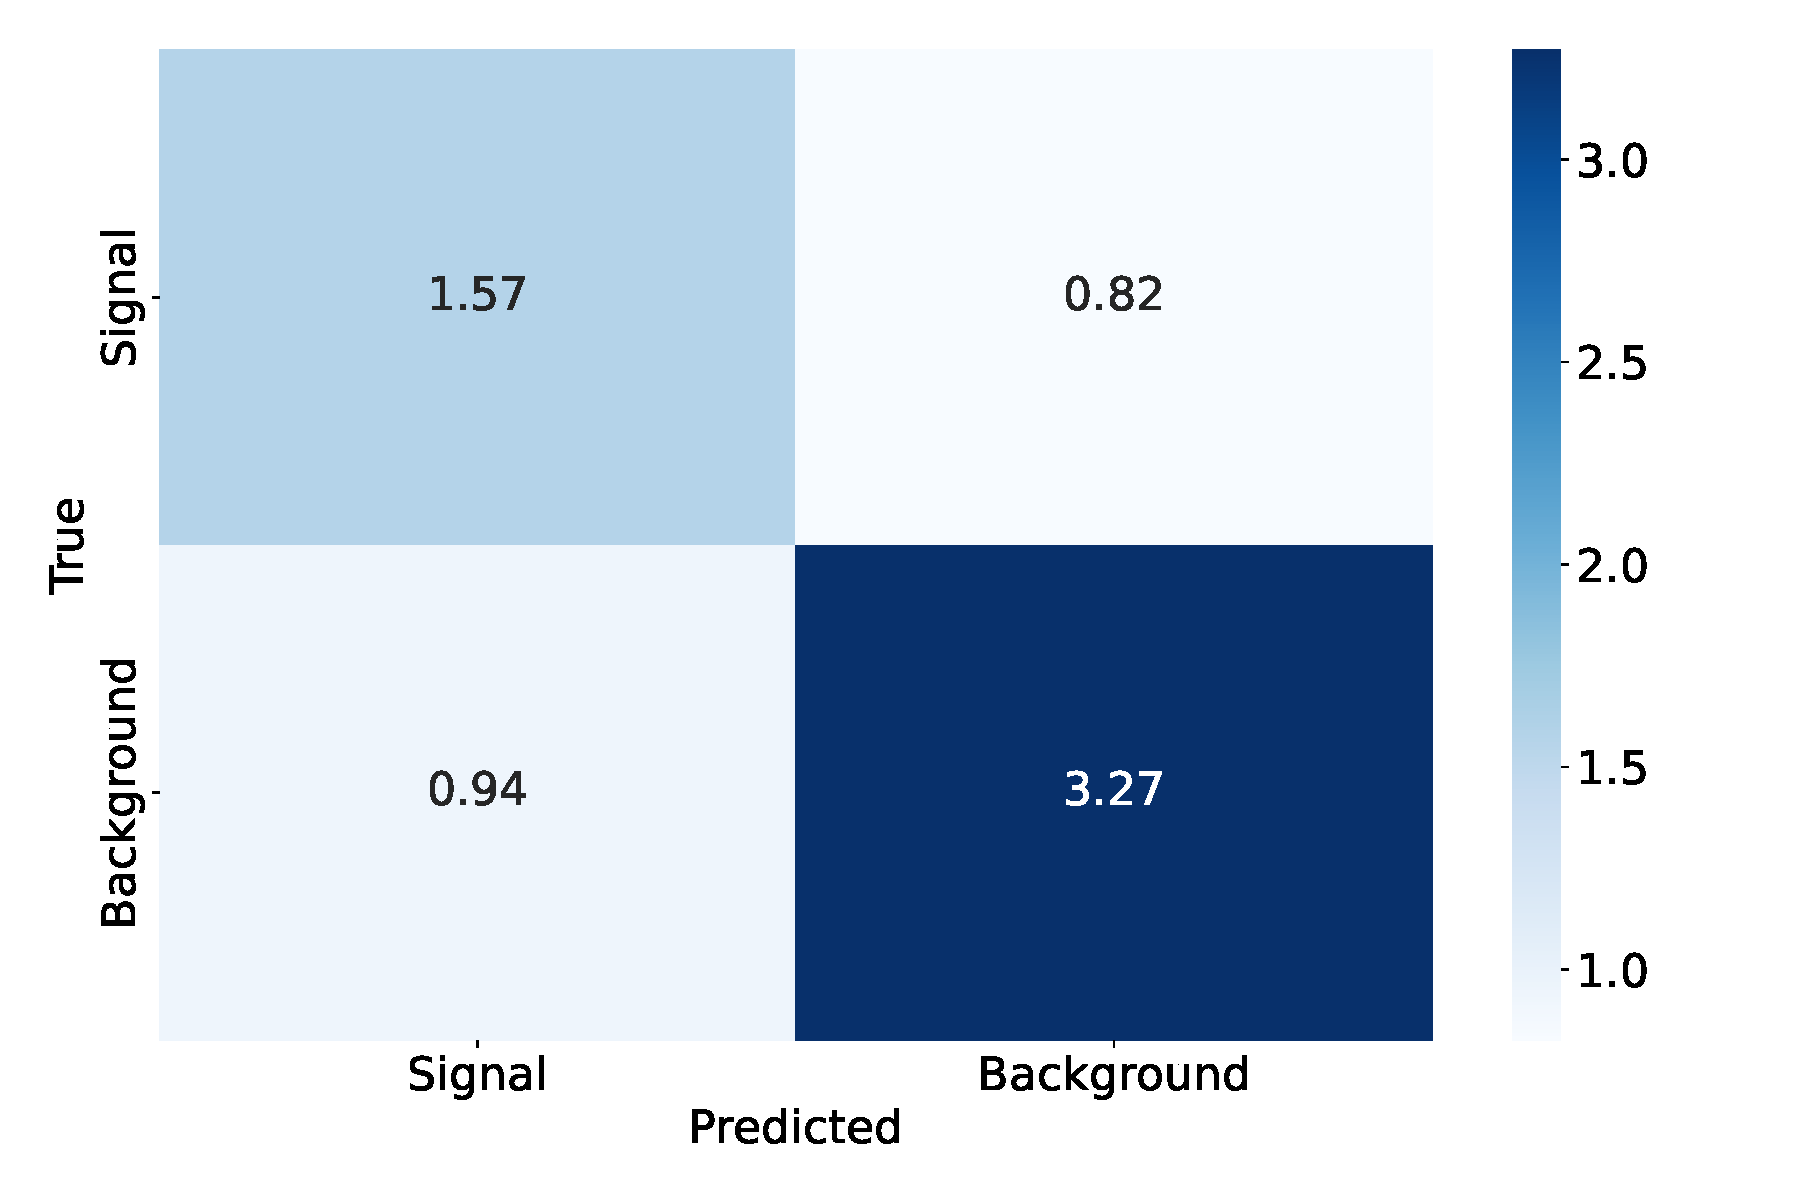
\includegraphics[trim=0.5cm 0 2cm 0, clip, width=0.8\textwidth]{figures/ml/cm/signal_argmax.pdf}
    \caption[Confusion matrix for a binary classification task]
    {Confusion matrix for a binary classification task. This confusion matrix is produced using 5-blocks
        \gls{ftt} (\autoref{sec:ftt}) trained on the extended training set (\autoref{sec:extended-set}) evaluated on the
        validation set, that contains 20\% of the \gls{sr} events. Signal refers to \tth, and background refers to all
        the other classes. The $\arg\max$ classification strategy was used.  Note that the classifier was \emph{trained}
        to differentiate between all the classes, but during evaluation, all the non-\tth events are grouped together.}
    \label{fig:cm}
\end{figure}

Binary confusion matrix naturally extends to a multi-class formulation (\autoref{fig:cm-muli}), leading to a
$|\classY| \times |\classY|$ matrix for a $|\classY|$-class classification task:

\begin{equation}
    \Cmulti_{ij} = \sum_{k=1}^{|\classY|} w_k \llbracket y_k = i \land \hat{y}_k = j \rrbracket\,,
\end{equation}

where $i$ and $j$ are the true and predicted classes, respectively. The diagonal elements of the matrix correspond to
the correctly classified events, while the off-diagonal elements correspond to the misclassified events. The
multi-class confusion matrix is not symmetric, and the sum of the elements in each row is equal to the number of events
in the corresponding true class.

\begin{figure}[htb]
    \centering
    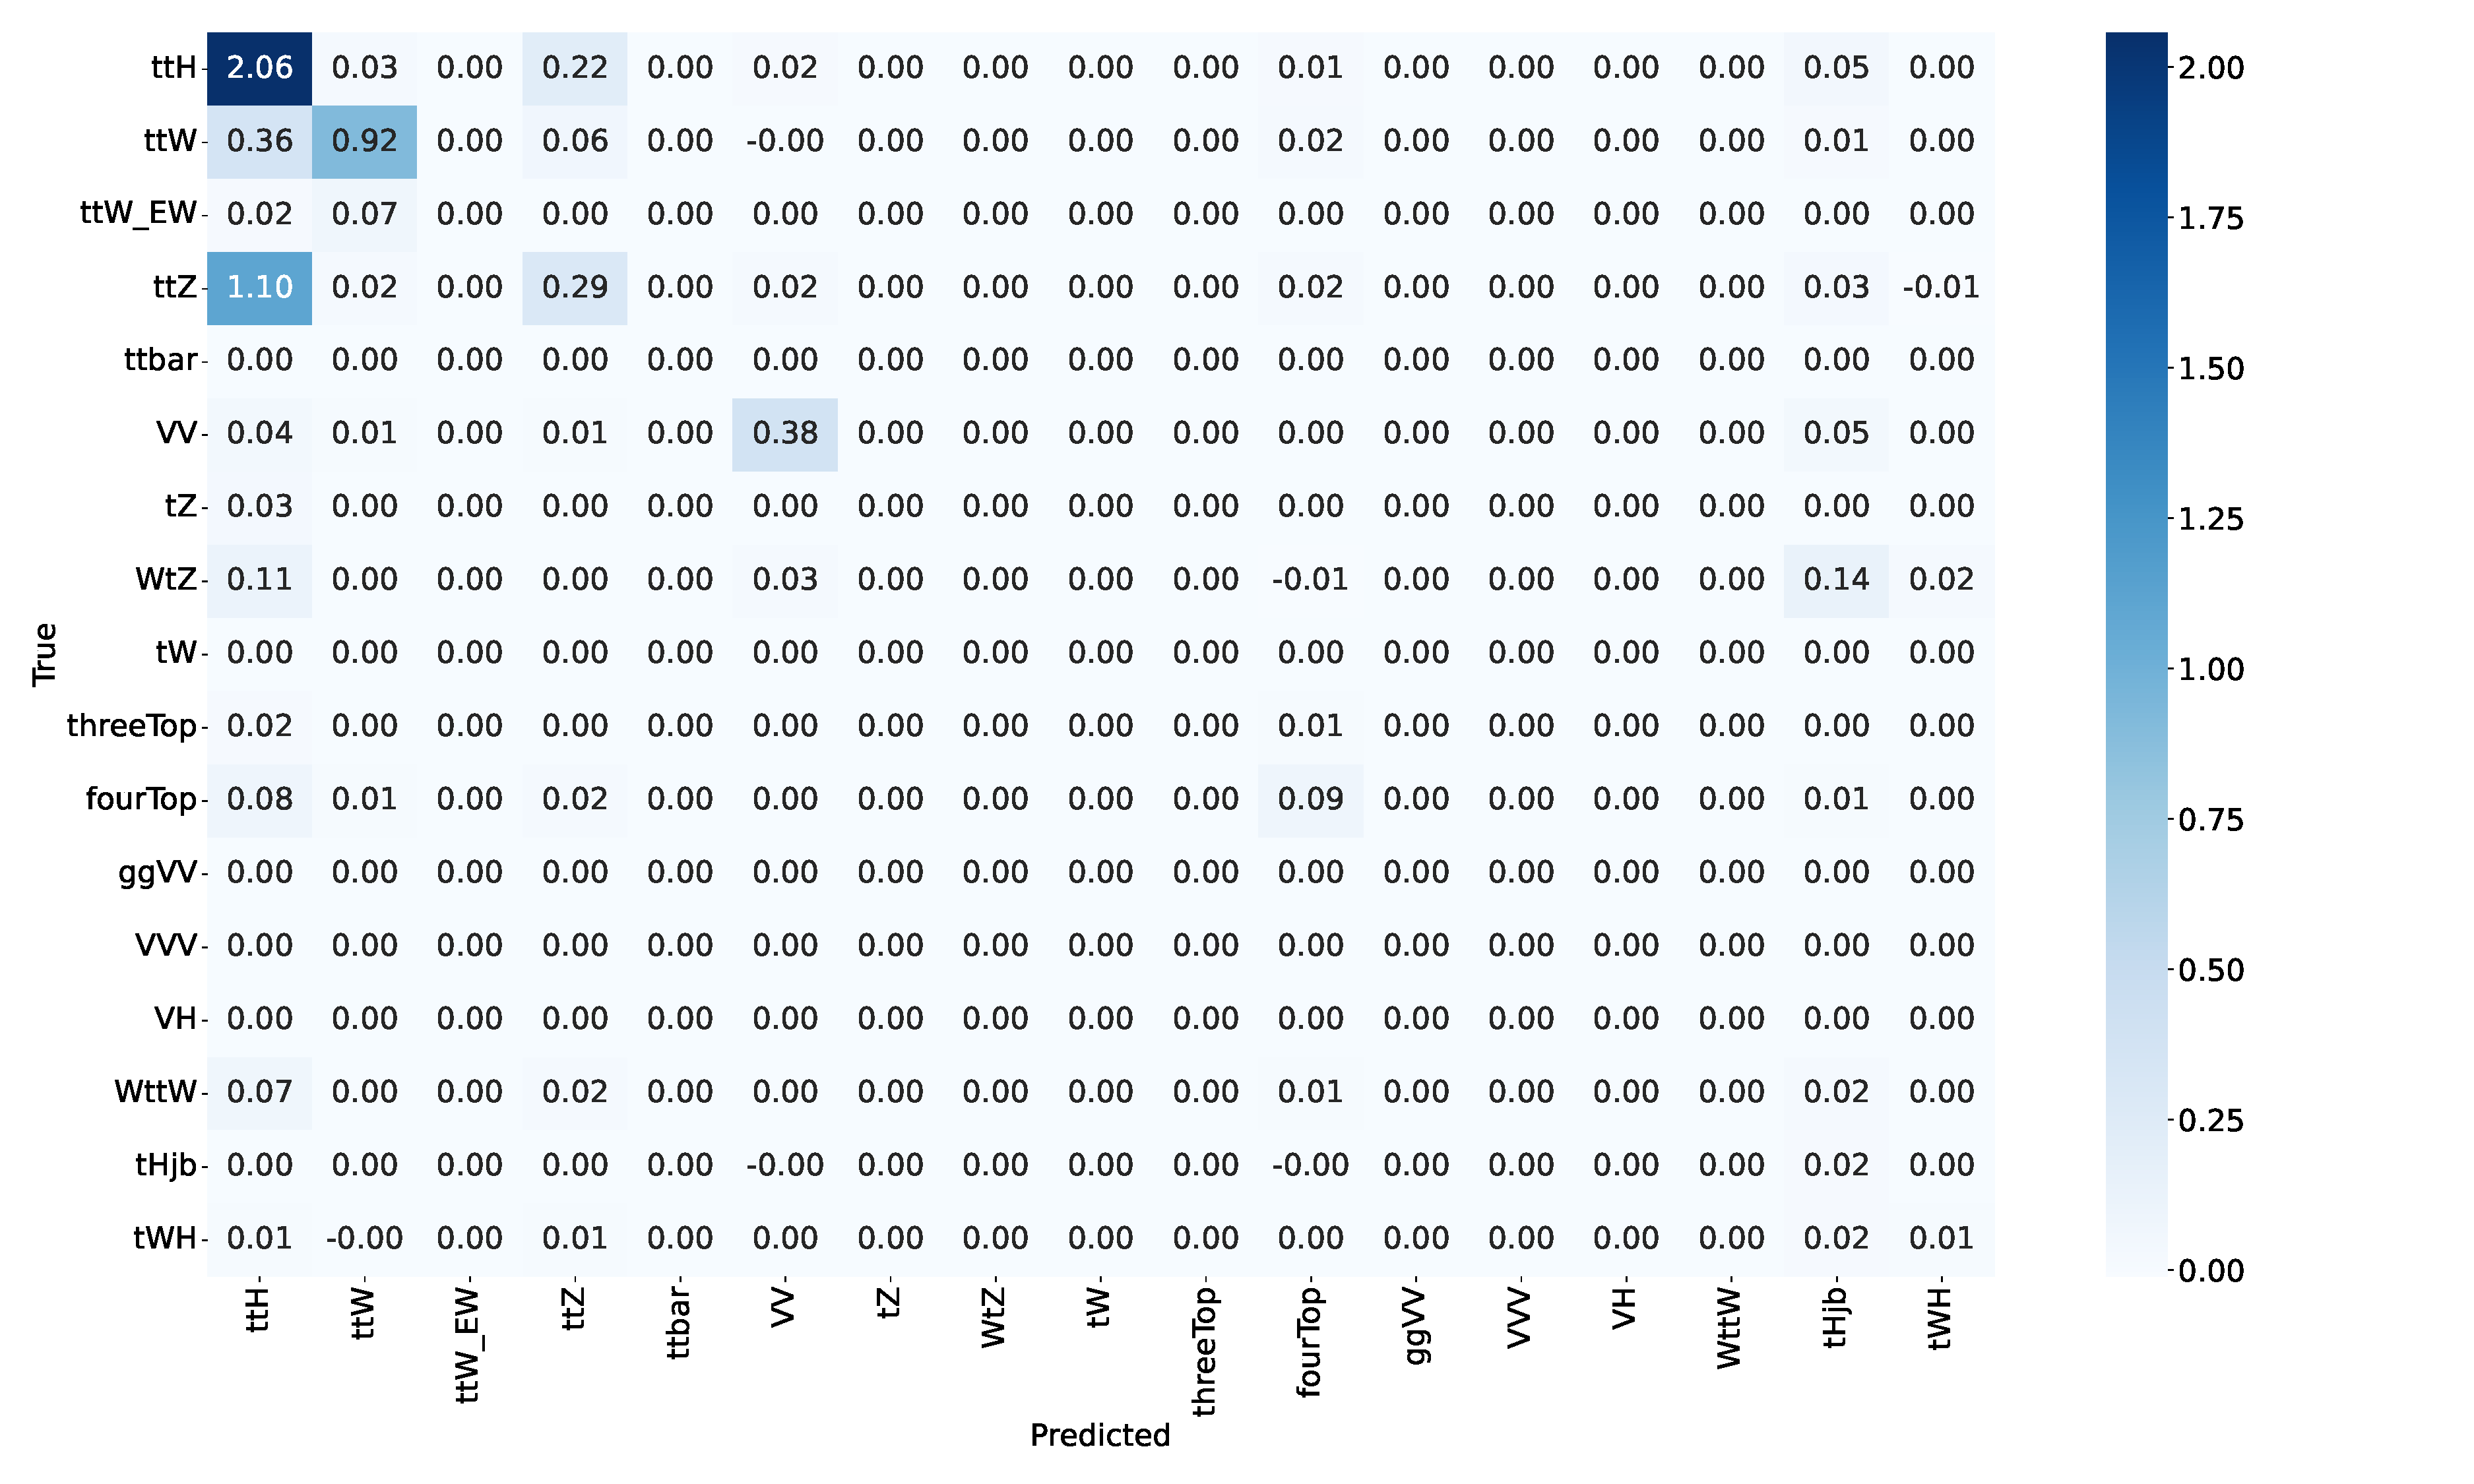
\includegraphics[trim=0.5cm 0 6cm 0, clip, width=\textwidth]{figures/ml/cm/all_argmax.pdf}
    \caption[Confusion matrix for a multi-class classification task]
    {Confusion matrix for a multi-class classification task. This confusion matrix is produced using 5-blocks
        \gls{ftt} (\autoref{sec:ftt}) trained on the extended training set (\autoref{sec:extended-set}). The
        $\arg\max$ classification strategy was used.}
    \label{fig:cm-muli}
\end{figure}

The confusion matrix serves as the basis for several other performance metrics, including accuracy, F1 score, and area
under the \gls{roc} curve (AUC-ROC).

\subsubsection{Accuracy: The Proportion of Correct Predictions}

Accuracy is the most intuitive performance metric. It is the ratio of the number of correctly classified examples
to the total number of examples (called events in particle physics). Accuracy is calculated trivially from the confusion
matrix:

\begin{align}
    \acc  = \frac{\trace \C_{ii}}{\sum_{i=1}^\classY \sum_{j=1}^\classY \C_{ij}}\,,
\end{align}

While accuracy is straightforward and commonly used, it may not always be the most representative metric, especially in
cases where the classes are imbalanced. Consider the example of our particle physics problem where we are searching for
\tth events and suppose that 90\% of the events are background and only 10\% are signal. A naïve classifier that
always predicts the background class would achieve an accuracy of 90\%. However, such a classifier would be entirely
unhelpful for the task at hand since it fails to identify any \tth events.

Certainly, the accuracy is not entirely without value, and there are contexts where it might still be useful. Even in
imbalanced scenarios, accuracy can provide a general sense of how often the classifier is correct across both the
majority and minority classes. While it may not provide a nuanced view of performance on the minority class (such as
\tth events in our case), it still provides information on the overall hit rate of correct predictions.

Additionally, in scenarios where the cost of false positives and false negatives are roughly equivalent, or when the
class distribution in the model's operational environment matches the training data, accuracy might still be a relevant
metric. It offers a quick and easily interpretable measure of performance.

However, in the specific context of searching for rare or significant events, such as \tth in particle physics, relying
solely on accuracy can be misleading. It would typically be considered alongside other metrics that give more insight
into the performance on the class of interest. Thus, while accuracy may not be the most representative metric in such
cases, it might still hold some value as part of a broader evaluation framework.

\subsubsection{Precision and Recall}

Two other important metrics which are derived from the confusion matrix are precision and recall, which are particularly
useful when dealing with imbalanced classes.

\paragraph{Precision} is the proportion of TP to all \emph{predicted} positives. Specifically, in our case, it is the
ratio of the correctly classified \tth events, to all events classified (or misclassified) as \tth. From here on, we
assume $y_1 = \tth$, and so the true \tth events correspond to the first row of the confusion matrix, while predicted
\tth events correspond to the first column. Precision is then given by

\begin{align}
    \text{Precision} = \frac{\C_{11}}{\sum_{j=1}^\classY \C_{1j}}\,.
\end{align}

\paragraph{Recall} (or sensitivity) is the proportion of TP to all \emph{actual} positives. In our case, it is the ratio
of the correctly classified \tth events to all actual \tth events (which the model might have missed by classifying them
as background). Recall is given by

\begin{align}
    \text{Recall} = \frac{\C_{11}}{\sum_{i=1}^\classY \C_{i1}}\,.
\end{align}

Precision tells us how reliable our positive predictions are,
while recall informs us how many of the actual \tth events we were able to detect. Both these metrics provide
complementary insights, and understanding the trade-off between them is essential in many real-world classification
tasks. Next, we will introduce the F1 score, a metric that combines both precision and recall to provide a balanced view
of the model's performance on both fronts.

\subsubsection{F1 Score: The Balance Between Precision and Recall}

The F1 score is the harmonic mean of precision and recall, providing a balance between the two. It is calculated as:

\begin{equation}
    \text{F1 score} = 2 \cdot \frac{\text{Precision} \cdot \text{Recall}}{\text{Precision} + \text{Recall}}
\end{equation}

\subsubsection{ROC Curve and AUC: The Trade-off Between Sensitivity and Specificity}

The \gls{roc} curve is a plot of the true positive rate (recall or sensitivity) against
the false positive rate (1 - specificity) for different classification thresholds. The area under the ROC curve
(AUC-ROC) measures the classifier's ability to distinguish between classes. A perfect classifier has an AUC-ROC of 1,
while a random classifier has an AUC-ROC of 0.5. The ROC curves for the \tth and two most dominant background processes
\ttw and \ttz are shown in \autoref{fig:rocs}.

\begin{figure}[htb]
    \centering
    \begin{subfigure}{0.32\textwidth}
        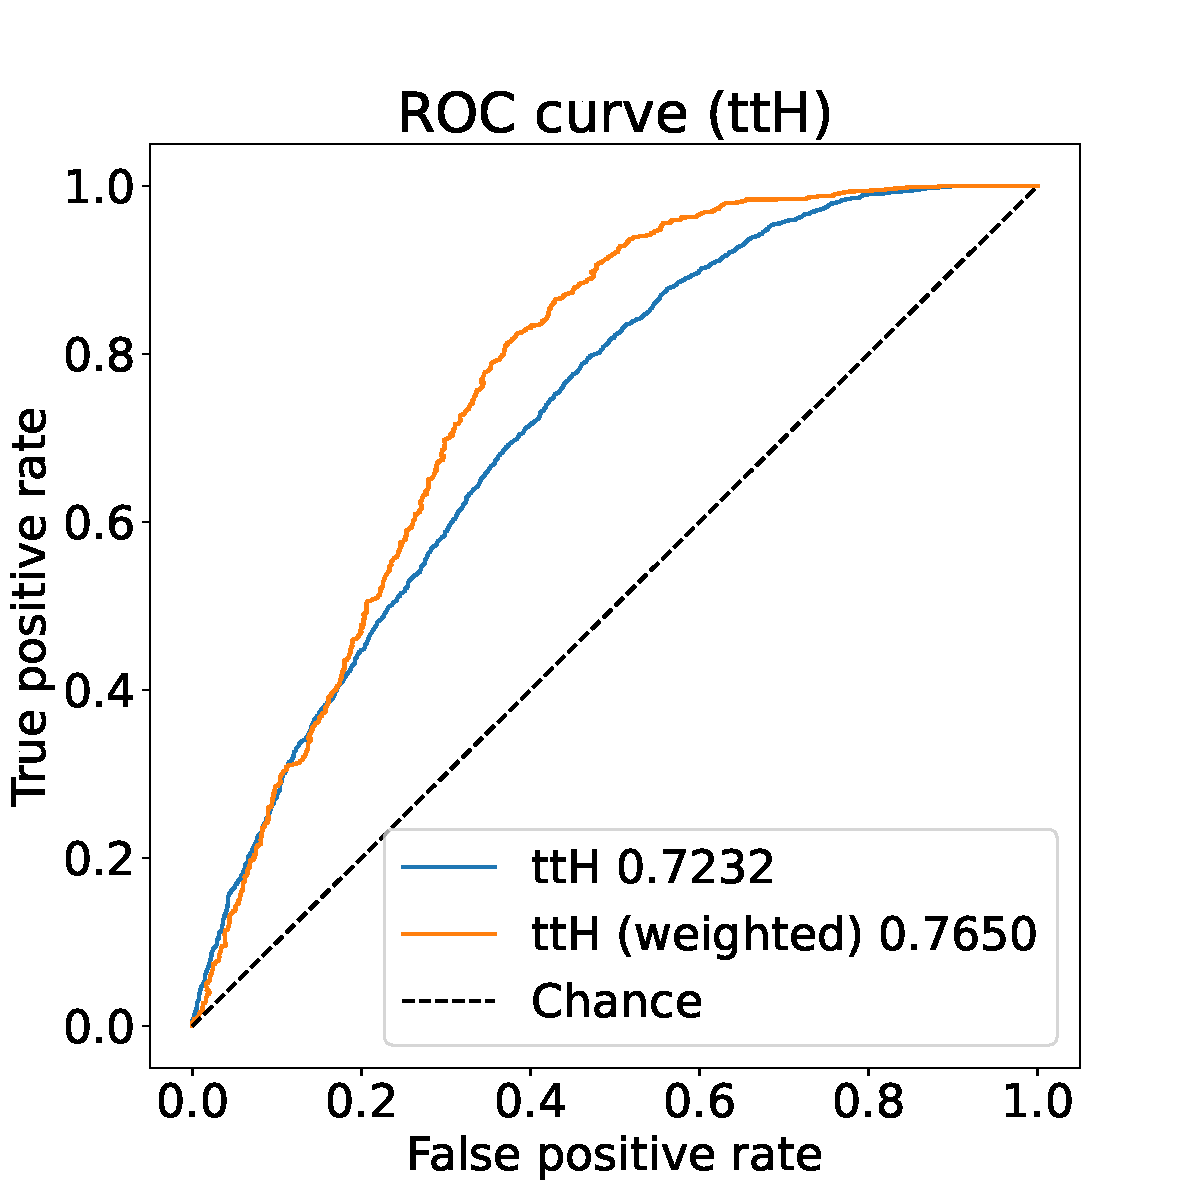
\includegraphics[width=\linewidth]{figures/ml/roc/ttH.pdf}
        \caption{\tth}
        \label{fig:roc-tth}
    \end{subfigure}
    \begin{subfigure}{0.32\textwidth}
        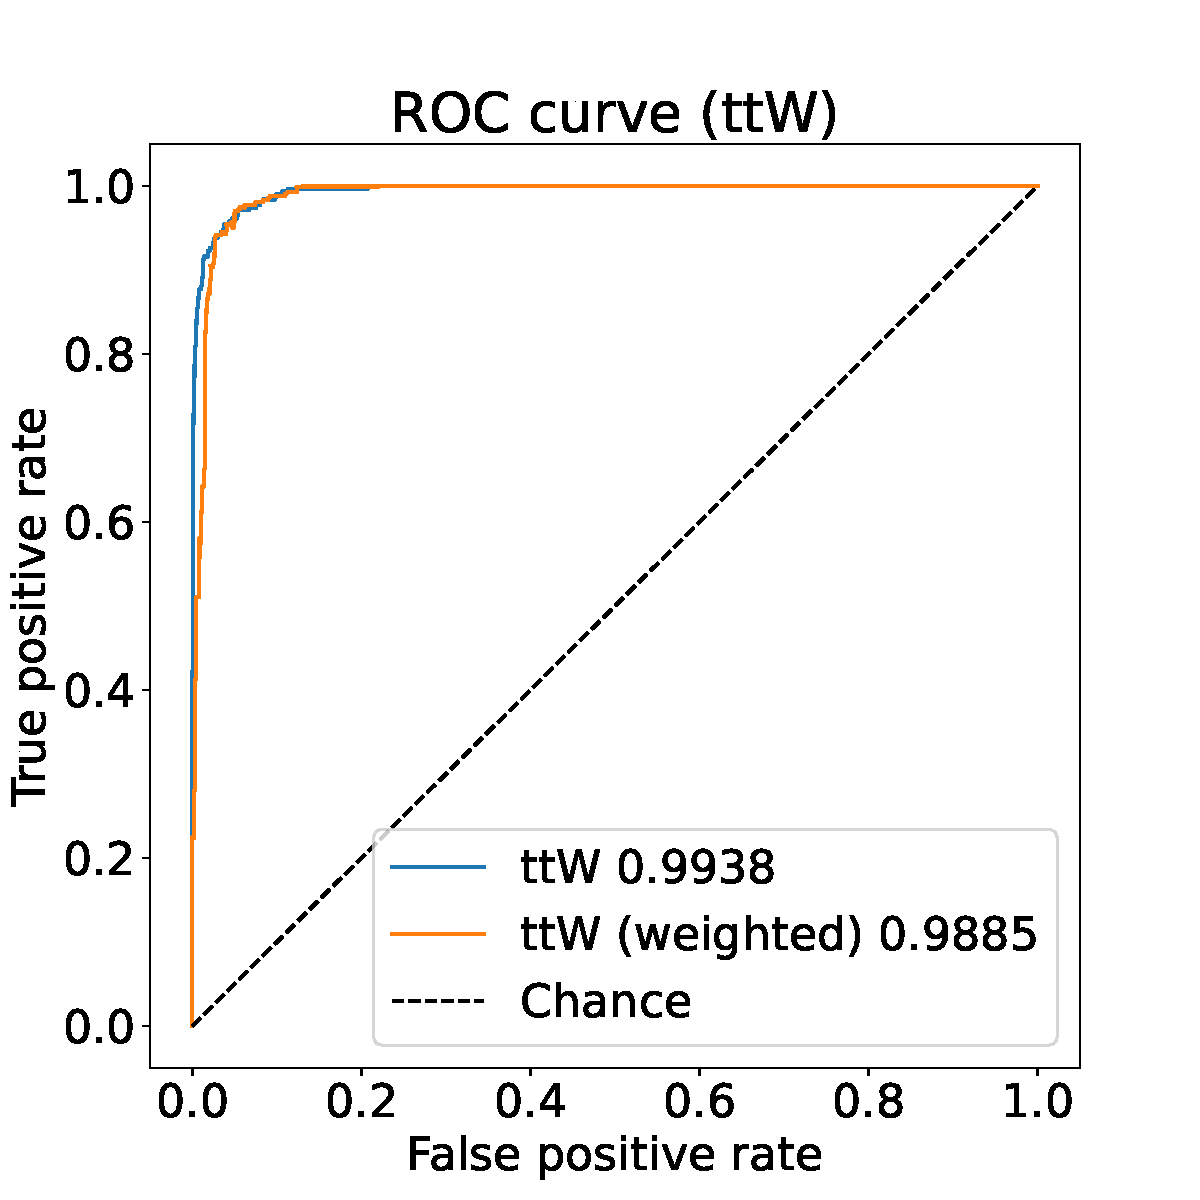
\includegraphics[width=\linewidth]{figures/ml/roc/ttW.pdf}
        \caption{\ttw}
        \label{fig:roc-ttw}
    \end{subfigure}
    \begin{subfigure}{0.32\textwidth}
        \includegraphics[width=\linewidth]{figures/ml/roc/ttZ.pdf}
        \caption{\ttz}
        \label{fig:roc-ttz}
    \end{subfigure}
    \caption[\acrshort{roc} curves for \tth, \ttz, and \ttz]
    {\gls{roc} curves for the \tth, \ttw, and \ttz computed using one process versus all other processes. The curves are produced
        using 5-blocks \gls{ftt} (\autoref{sec:ftt}) trained on the extended training set (\autoref{sec:extended-set}).
        We provide both the \glspl{roc} computed with the weighted and unweighted confusion matrices for completeness
        and comparison with the previous analysis, however, we emphasize that the weighted \glspl{roc} are the ones that
        should be used always.}
    \label{fig:rocs}
\end{figure}


These metrics, combined with the loss function, provide a comprehensive view of the classifier's performance and guide
the optimization process during training. They also provide a robust measure for comparing different classifiers or the
same classifier with different hyperparameters. Generally, one should examine all of these metrics to get a complete
picture of the classifier's performance.

% Include the architectures section
\section{V8 adaptation}

\section{\gls{sr} cut expression}
\label{appendix:cut-expression}

{\scriptsize
    \begin{verbatim}
    custTrigMatch_LooseID_FCLooseIso_DLT
    && (dilep_type && (lep_ID_0*lep_ID_1)>0)
    && ((lep_Pt_0 >= 10e3 && lep_Pt_1 >= 10e3) && (fabs(lep_Eta_0) <= 2.5 && fabs(lep_Eta_1) <= 2.5)
        && ((abs(lep_ID_0) == 13 && lep_isMedium_0 && lep_isolationLoose_VarRad_0 && passPLIVTight_0)
            || ((abs(lep_ID_0) == 11 && lep_isTightLH_0 && lep_isolationLoose_VarRad_0 && passPLIVTight_0
                && lep_ambiguityType_0 == 0 && lep_chargeIDBDTResult_recalc_rel207_tight_0 > 0.7)
                && ((!(!(lep_Mtrktrk_atConvV_CO_0 < 0.1 && lep_Mtrktrk_atConvV_CO_0 >= 0 && lep_RadiusCO_0 > 20)
                    && (lep_Mtrktrk_atPV_CO_0 < 0.1 && lep_Mtrktrk_atPV_CO_0 >= 0)))
                    && !(lep_Mtrktrk_atConvV_CO_0 <0.1 && lep_Mtrktrk_atConvV_CO_0 >= 0 && lep_RadiusCO_0 > 20))))
            && ((abs(lep_ID_1) == 13 && lep_isMedium_1 && lep_isolationLoose_VarRad_1 && passPLIVTight_1)
                || ((abs(lep_ID_1) == 11 && lep_isTightLH_1 && lep_isolationLoose_VarRad_1 && passPLIVTight_1
                    && lep_ambiguityType_1 == 0 && lep_chargeIDBDTResult_recalc_rel207_tight_1 > 0.7)
                    && ((!(!(lep_Mtrktrk_atConvV_CO_1 < 0.1 && lep_Mtrktrk_atConvV_CO_1 >= 0 && lep_RadiusCO_1 > 20)
                        && (lep_Mtrktrk_atPV_CO_1 < 0.1 && lep_Mtrktrk_atPV_CO_1 >= 0)))
                        && !(lep_Mtrktrk_atConvV_CO_1 < 0.1 && lep_Mtrktrk_atConvV_CO_1 >= 0 && lep_RadiusCO_1 > 20)))))
    && nTaus_OR==1
    && nJets_OR_DL1r_85>=1
    && nJets_OR>=4
    && ((dilep_type==2) || abs(Mll01-91.2e3)>10e3)
\end{verbatim}
}

We have kept the cuts the same as \cite{severin}, except for the cut on the \verb|nJets_OR| to \verb|>=4| to keep
consistent definition \gls{sr} definition across the group \todo{refer to the BDT group - how?}.

\section{Yields Plots}
\label{appendix:yields}

\begin{figure}[htb!]
    \centering
    \begin{subfigure}{0.45\textwidth}
        \includegraphics[width=\linewidth]{figures/yields/lep-pt-0.pdf}
        \caption{Distribution of the transverse momentum of the leading lepton.}
    \end{subfigure}\hfill%
    \begin{subfigure}{0.45\textwidth}
        \includegraphics[width=\linewidth]{figures/yields/lep-pt-1.pdf}
        \caption{Distribution of the transverse momentum of the subleading lepton.}
    \end{subfigure}
\end{figure}

\begin{figure}[htb!]
    \centering
    \begin{subfigure}{0.45\textwidth}
        \includegraphics[width=\linewidth]{figures/yields/n-jets.pdf}
        \caption{Distribution of the number of jets.}
    \end{subfigure}\hfill%
    \begin{subfigure}{0.45\textwidth}
        \includegraphics[width=\linewidth]{figures/yields/n-bjets.pdf}
        \caption{Distribution of the number of $b$-jets.}
    \end{subfigure}
\end{figure}

\begin{figure}[htb!]
    \centering
    \begin{subfigure}{0.45\textwidth}
        \includegraphics[width=\linewidth]{figures/yields/tau-width.pdf}
        \caption{Distribution of the $\tau$-jet width.}
    \end{subfigure}\hfill%
\end{figure}
\subsection{List of samples by each process}

The root directory for the files is:

{\small
\verb|/eos/atlas/atlascerngroupdisk/phys-higgs/HSG8/multilepton_ttWttH/v08/v0801/systematics-full/nominal|
}

The list of samples is given in \hyperref[tab:samples]{Table~\ref*{tab:samples}}.

\newpage

\begin{table}[h!]
    \centering
    \renewcommand{\arraystretch}{1.5}
    \caption{List of samples by each process}
    \label{tab:samples}
    \begin{tabular}{p{1.5cm}p{13.5cm}}
        \toprule
        Process      & \gls{dsid}                                                           \\
        \midrule
        $t\bar{t}H$  & p4498/346343, p4498/346344, p4498/346345                             \\
        $t\bar{t}W$  & p4416/700168, p4590/700205                                           \\
        $t\bar{t}Z$  & p4416/700168                                                         \\
        $t\bar{t}$   & p4308/410470                                                         \\
        $VV$         & \input{samples/VV.tex}                                               \\
        $ggVV$       & p4308/345705, p4396/345706, p4396/345715, p4396/345718, p4396/345723 \\
        $Zjets$      & \input{samples/Zjets.tex}                                            \\
        $Wjets$      & \input{samples/Wjets.tex}                                            \\
        $tW$         & p4308/410646, p4308/410647                                           \\
        $threeTop$   & p4308/304014                                                         \\
        $fourTop$    & p4308/410080                                                         \\
        $t\bar{t}WW$ & p4308/410081                                                         \\
        $tZ$         & p4308/410560                                                         \\
        $WtZ$        & p4308/410408                                                         \\
        $VVV$        & \input{samples/VVV.tex}                                              \\
        $VH$         & p4308/342284, p4308/342285                                           \\
        $tHjb$       & p4308/346799\_AF                                                     \\
        $tWH$        & p4308/346678\_AF                                                     \\
        \bottomrule
    \end{tabular}
\end{table}

\newpage
\subsection{Distribution of the variables inside \gls{sr}}

The following figures (\autoref{fig:distributions1} and \autoref{fig:distributions2}) show the distributions of some variables
of interest inside \gls{sr}.

\captionsetup[subfigure]{justification=centering}
\begin{figure}[htb!]
    \centering
    \begin{subfigure}{0.45\textwidth}
        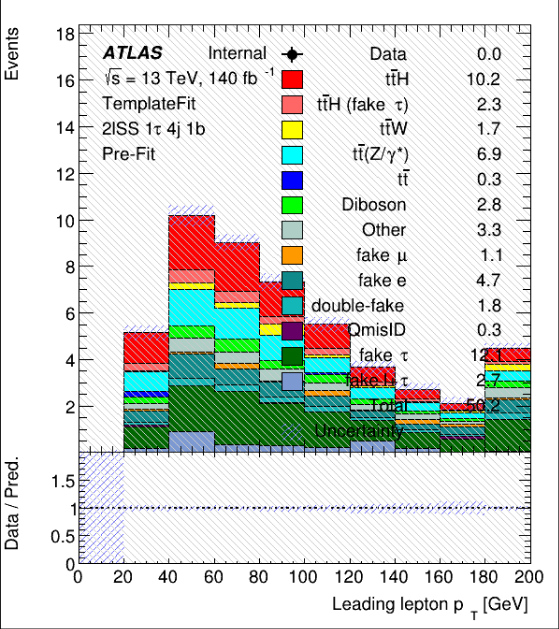
\includegraphics[width=\linewidth]{figures/plots/histograms/lep_pt_0.png}
        \caption{Distribution of the transverse momentum of the leading lepton.}
        \label{fig:lep_pt_0}
    \end{subfigure}\hfill%
    \begin{subfigure}{0.45\textwidth}
        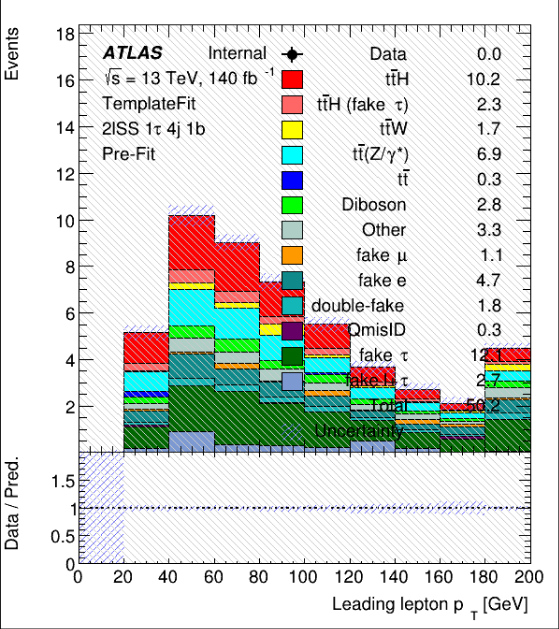
\includegraphics[width=\linewidth]{figures/plots/histograms/lep_pt_1.png}
        \caption{Distribution of the transverse momentum of the subleading lepton.}
        \label{fig:lep_pt_1}
    \end{subfigure}

    \vspace{0.5cm}

    \begin{subfigure}{0.45\textwidth}
        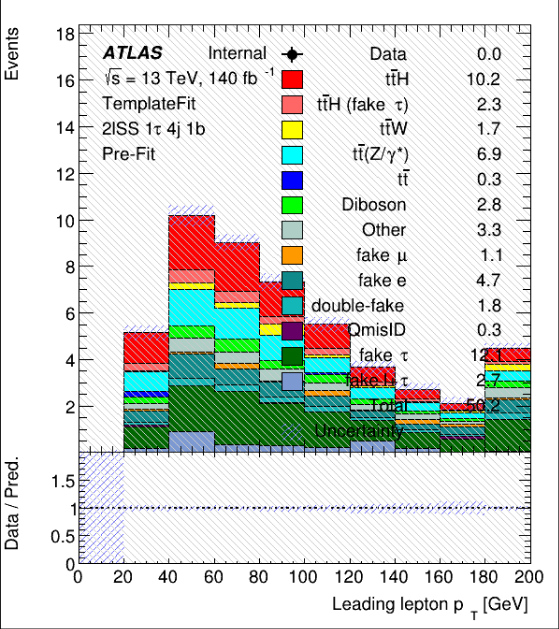
\includegraphics[width=\linewidth]{figures/plots/histograms/lep_Eta_0.png}
        \caption{Distribution of the pseudorapidity of the leading lepton.}
        \label{fig:lep_Eta_0}
    \end{subfigure}\hfill%
    \begin{subfigure}{0.45\textwidth}
        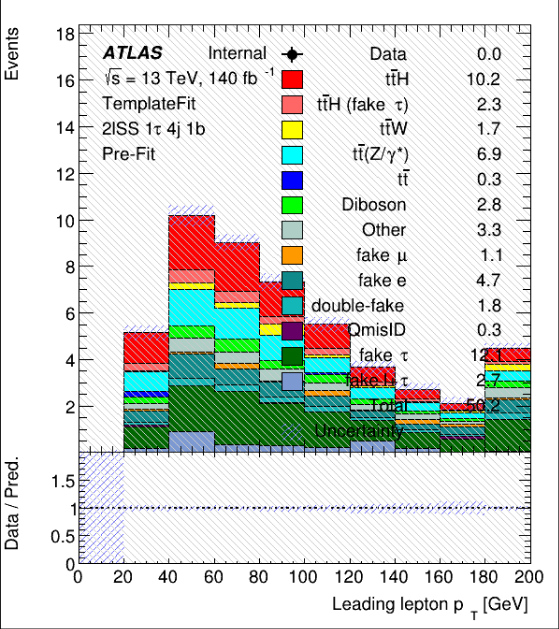
\includegraphics[width=\linewidth]{figures/plots/histograms/lep_Eta_1.png}
        \caption{Distribution of the pseudorapidity of the subleading lepton.}
        \label{fig:lep_Eta_1}
    \end{subfigure}
    \caption{Distributions of the variables inside \gls{sr} (part 1)}
    \label{fig:distributions1}
\end{figure}

\newpage

\begin{figure}[htb!]
    \centering
    \begin{subfigure}{0.45\textwidth}
        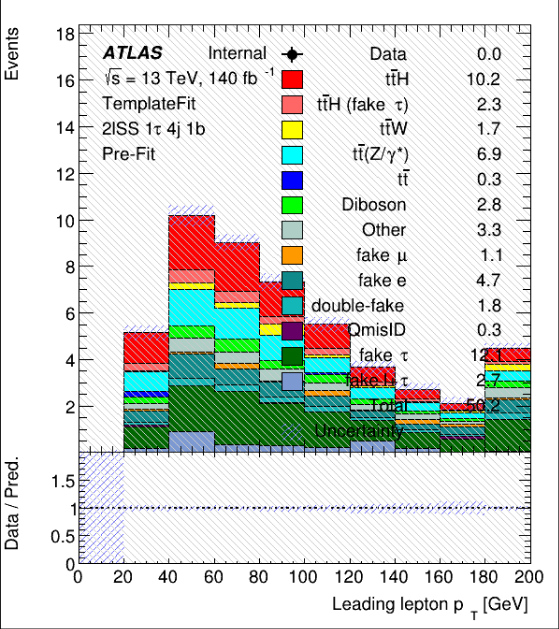
\includegraphics[width=\linewidth]{figures/plots/histograms/lep_Phi_0.png}
        \caption{Distribution of the azimuthal angle of the leading lepton.}
        \label{fig:lep_Phi_0}
    \end{subfigure}\hfill%
    \begin{subfigure}{0.45\textwidth}
        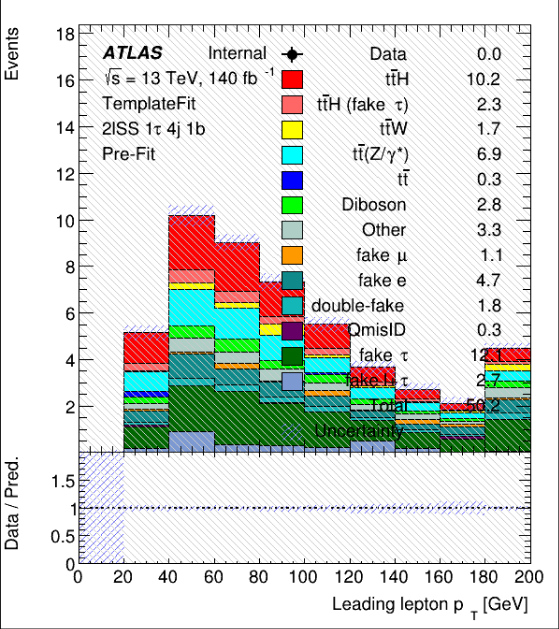
\includegraphics[width=\linewidth]{figures/plots/histograms/lep_Phi_1.png}
        \caption{Distribution of the azimuthal angle of the subleading lepton.}
        \label{fig:lep_Phi_1}
    \end{subfigure}

    \vspace{0.5cm}

    \begin{subfigure}{0.45\textwidth}
        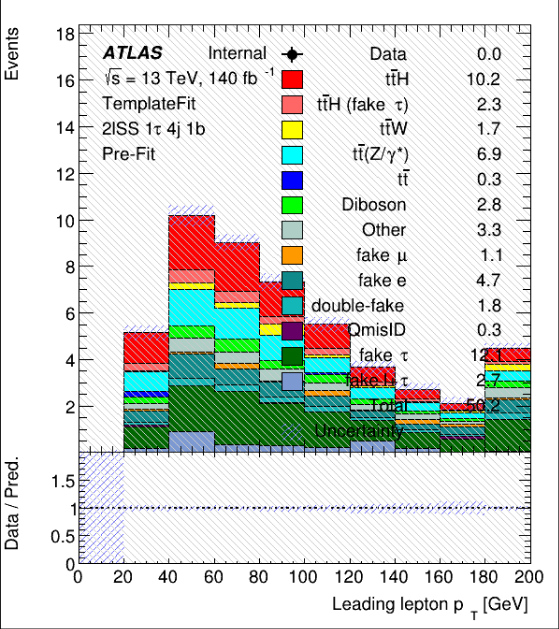
\includegraphics[width=\linewidth]{figures/plots/histograms/njets.png}
        \caption{Distribution of the number of jets.}
        \label{fig:njets}
    \end{subfigure}\hfill%
    \begin{subfigure}{0.45\textwidth}
        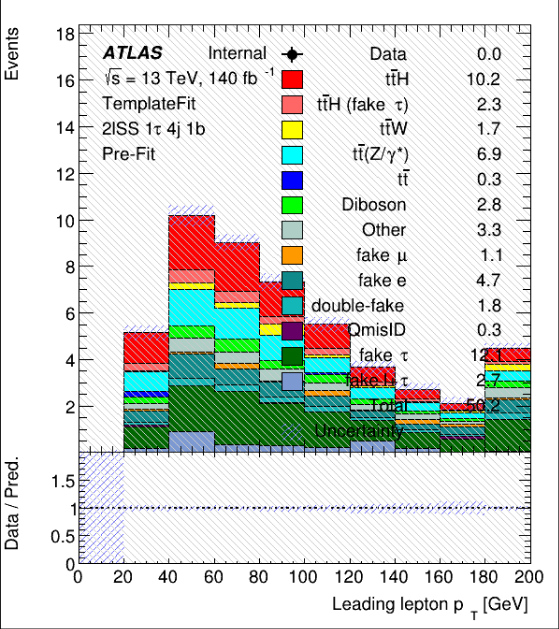
\includegraphics[width=\linewidth]{figures/plots/histograms/nbjets.png}
        \caption{Distribution of the number of $b$-jets.}
        \label{fig:nbjets}
    \end{subfigure}
    \caption{Distributions of the variables inside \gls{sr} (part 2)}
    \label{fig:distributions2}
\end{figure}

\begin{minipage}{0.45\textwidth}
    \centering
    \begin{tabular}{c|c|c|c|c}
        $t\bar{t}H$ & \textbf{v6} & \textbf{v8} &      &       \\
        \hline
        Weighted    & 1000        & 500         & -500 & -50\% \\
        Raw         & 1000        & 500         & -500 & -50\% \\
        \hline
    \end{tabular}
    \captionof{table}{Number of ttH events in the SR for v6 and v8.}
    \label{tab:ttH_event_numbers1}
\end{minipage}\hfill%
\begin{minipage}{0.45\textwidth}
    \centering
    \begin{tabular}{c|c|c|c|c}
        \gls{sr} & \textbf{v6} & \textbf{v8} &      &       \\
        \hline
        Weighted & 1000        & 500         & -500 & -50\% \\
        Raw      & 1000        & 500         & -500 & -50\% \\
        \hline
    \end{tabular}
    \captionof{table}{Number of all the events in the SR for v6 and v8.}
    \label{tab:ttH_event_numbers2}
\end{minipage}

\clearpage \subsection{Features used}

\subsubsection{\texttt{lep\_E\_X}} The energy of the Xth lepton.

\subsubsection{\texttt{DRjj\_lead}} $\Delta R$ between the two leading jets. $\Delta R$ is a distance metric in the
$\eta-\phi$ space frequently used in particle physics.

\subsubsection{\texttt{Ptll01}} The transverse momentum of the dilepton system made up of the two leading leptons.

\subsubsection{\texttt{lep\_nTrackParticles\_X}} The number of track particles associated with the Xth lepton.

\subsubsection{\texttt{custTrigMatch\_LooseID\_FCLooseIso\_DLT}} Custom trigger matching for loosely identified and loosely
isolated leptons, likely related to the dilepton trigger

\subsubsection{\texttt{Mll01}} The invariant mass of the two leading leptons.

\subsubsection{\texttt{Mlll012}} The invariant mass of the three leading leptons.

\subsubsection{\texttt{total\_charge}} The sum of the electric charges of the particles in the event.

\subsubsection{\texttt{HT}} The scalar sum of the transverse momenta of all jets in the event.

\subsubsection{\texttt{HT\_lep}} The scalar sum of the transverse momenta of all leptons in the event.

\subsubsection{\texttt{lep\_Eta\_X}} The pseudorapidity of the Xth lepton.

\subsubsection{\texttt{nTaus\_OR\_Pt25}} The number of overlapping-removed taus with a transverse momentum above 25 GeV.

\subsubsection{\texttt{nFwdJets\_OR}} The number of overlapping-removed forward jets.

\subsubsection{\texttt{MLepMet}} The invariant mass of a lepton and the missing transverse energy vector.

\subsubsection{\texttt{taus\_DL1r\_X}} The DL1r score for the Xth tau.

\subsubsection{\texttt{lep\_isolationLoose\_VarRad\_X}} Indicates whether a lepton (where X refers to the lepton index)
passes an isolation cut with a variable radius. Looser isolation cuts allow more nearby activity in the detector.

\subsubsection{\texttt{lep\_EtaBE2\_X}} The pseudorapidity of the Xth lepton in the second layer of the electromagnetic
calorimeter.

\subsubsection{\texttt{HT\_fwdJets}} The scalar sum of the transverse momenta of all forward jets in the event.

\subsubsection{\texttt{taus\_width\_X}} The width of the Xth tau.

\subsubsection{\texttt{nJets\_OR\_DL1r\_85}} Count of jets that pass overlap removal (OR) and are b-tagged according to the
DL1r algorithm at the 85\% working point.

\subsubsection{\texttt{lep\_nInnerPix\_X}} Number of hits in the inner pixel detector associated with the lepton, where X
refers to the lepton index.

\subsubsection{\texttt{met\_phi}} The azimuthal angle of the missing transverse energy in the event.

\subsubsection{\texttt{DeltaR\_max\_lep\_bjet77}} The maximum DeltaR value between a lepton and a b-tagged jet. The "77"
may refer to the working point of the b-tagging algorithm.

\subsubsection{\texttt{MbX}} Invariant mass associated with the leading b-jet in the event

\subsubsection{\texttt{lep\_RadiusCO\_X}} Possibly the radius of the cone used for isolation of the lepton, or
alternatively a parameter associated with the trajectory of the lepton.

\subsubsection{\texttt{lep\_Mtrktrk\_atConvV\_CO\_X}} The invariant mass of track pairs at the conversion vertex for lepton
X. This might be related to photon conversions into an electron-positron pair.

\subsubsection{\texttt{lep\_Z0SinTheta\_X}} The z0 impact parameter times the sine of the lepton's polar angle.

\subsubsection{\texttt{lep\_Pt\_X}} The transverse momentum of the Xth lepton.

\subsubsection{\texttt{mjjMax\_frwdJet}} The maximum invariant mass of a pair of forward jets.

\subsubsection{\texttt{dilep\_type}} The type of dilepton event (e.g., $ee$, $\mu e$, $\mu \mu$).

\subsubsection{\texttt{eta\_frwdjet}} The pseudorapidity of the forward jet.

\subsubsection{\texttt{Mlb}} Invariant mass of a lepton and a b-jet.

\subsubsection{\texttt{taus\_RNNJetScoreSigTrans\_X}} Transformed RNN-based score for tau lepton, possibly to better
separate signal from background.

\subsubsection{\texttt{minDeltaR\_LJ\_X}} The minimum $\Delta R$ distance between the Xth lepton and any jet in the event.

\subsubsection{\texttt{nTaus\_OR}} Number of tau leptons that pass overlap removal. Overlap removal is a step in particle
reconstruction where, for instance, an object identified as both a jet and a tau would be considered only as one or the
other.

\subsubsection{\texttt{DeltaR\_min\_lep\_jet}} The minimum $\Delta R$ distance between a lepton and a jet in the event.

\subsubsection{\texttt{lep\_sigd0PV\_X}} Significance of the transverse impact parameter (d0) of the lepton X with respect
to the primary vertex (PV). This is a common variable for distinguishing prompt particles produced in the primary
collision from secondary particles produced in a decay.

\subsubsection{\texttt{taus\_eta\_X}} The pseudorapidity of the Xth tau.

\subsubsection{\texttt{HT\_jets}} The scalar sum of the transverse momenta of all jets (not forward jets) in the event.

\subsubsection{\texttt{lep\_Phi\_X}} The azimuthal angle (in radians) of the Xth lepton.

\subsubsection{\texttt{bTagSF\_weight\_DL1r\_85}} A weight applied to events based on the scale factor for b-tagging using
the DL1r algorithm at an 85\% efficiency working point. This scale factor corrects the b-tagging efficiency in Monte
Carlo simulations to match that observed in real data.

\subsubsection{\texttt{lep\_chargeIDBDTResult\_recalc\_rel207\_tight\_X}} The outcome of a BDT-based charge identification
for a lepton, recalculated with some specific settings, and applying a 'tight' threshold.

\subsubsection{\texttt{taus\_phi\_X}} The azimuthal angle (in radians) of the Xth tau.

\subsubsection{\texttt{taus\_passJVT\_X}} A boolean flag indicating whether the Xth tau passes the jet vertex tightness
(JVT) requirement.

\subsubsection{\texttt{jets\_eta}} The pseudorapidity of the jets (array).

\subsubsection{\texttt{taus\_charge\_X}} The charge of the Xth tau.

\subsubsection{\texttt{passPLIVTight\_X}} Boolean flag indicating if a lepton with high transverse momentum passes the
"tight" criteria of the Prompt Lepton Veto (PLIV), a tool for identifying non-prompt light leptons.

\subsubsection{\texttt{lep\_Mtrktrk\_atPV\_CO\_X}} The invariant mass of track pairs at the primary vertex for lepton X.
This could be related to certain types of particle decays happening at the primary collision vertex.

\subsubsection{\texttt{taus\_JetRNNSigMedium\_X}} RNN-based score for tau lepton, used to distinguish tau leptons from
jets, with 'medium' selection criteria.

\subsubsection{\texttt{minOSMll}} The minimum invariant mass of oppositely-signed dilepton pairs.

\subsubsection{\texttt{lep\_ID\_X}} The identification number for the Xth lepton.

\subsubsection{\texttt{Mllll0123}} The invariant mass of the four leading leptons.

\subsubsection{\texttt{custTrigSF\_TightElMediumMuID\_FCLooseIso\_DLT}} Custom trigger scale factor, for events with a
tight electron and a medium muon, both of which are loosely isolated, likely related to the dilepton trigger (DLT).

\subsubsection{\texttt{best\_Z\_Mll}} The invariant mass of the dilepton system that is closest to the Z boson mass.

\subsubsection{\texttt{met\_met}} The missing transverse energy in the event.

\subsubsection{\texttt{MtLep1Met}} Transverse mass between the leading lepton and missing transverse energy. Transverse
mass is often used in searches for particles that decay to a lepton and a neutrino.

\subsubsection{\texttt{lep\_ambiguityType\_X}} Type of ambiguity for lepton identification, where X refers to the lepton
index. Ambiguity could arise from several factors, such as a single track matching with multiple reconstructed
particles.

\subsubsection{\texttt{jets\_phi}} The azimuthal angle (in radians) of the jets (array).

\subsubsection{\texttt{lep\_isMedium\_X}} Boolean flag indicating if a lepton passes the 'medium' selection criteria.

\subsubsection{\texttt{taus\_RNNJetScore\_X}} RNN-based score for tau lepton, used to distinguish tau leptons from jets.

\subsubsection{\texttt{MtLepMet}} The transverse mass of a lepton and the missing transverse energy vector.

\subsubsection{\texttt{DeltaR\_min\_lep\_jet\_fwd}} The minimum $\Delta R$ distance between a lepton and a forward jet in the event.

\subsubsection{\texttt{jets\_e}} The energy of the jets (array).

\subsubsection{\texttt{minOSSFMll}} The minimum invariant mass of oppositely-signed, same-flavor dilepton pairs.

\subsubsection{\texttt{nJets\_OR}} The number of overlapping-removed jets.

\subsubsection{\texttt{total\_leptons}} The total number of leptons in the event.

\subsubsection{\texttt{taus\_numTrack\_X}} The number of tracks associated with the Xth tau.

\subsubsection{\texttt{HT\_taus}} Scalar sum of the transverse momenta ($P_t$) of all tau leptons in the event.

\subsubsection{\texttt{taus\_passEleOLR\_X}} A boolean flag indicating whether the Xth tau passes the electron overlap
removal.

\subsubsection{\texttt{HT\_inclFwdJets}} The scalar sum of the transverse momenta of all jets, including forward jets, in
the event.

\subsubsection{\texttt{DRll01}} The $\Delta R$ distance between the two leading leptons.

\subsubsection{\texttt{taus\_JetRNNSigLoose\_X}} RNN-based score for tau lepton, used to distinguish tau leptons from
jets, with 'loose' selection criteria.

\subsubsection{\texttt{taus\_pt\_X}} The transverse momentum of the Xth tau.

\subsubsection{\texttt{bTagSF\_weight\_DL1r\_77}} A weight applied to events based on the scale factor for b-tagging using
the DL1r algorithm at an 77\% efficiency working point. This scale factor corrects the b-tagging efficiency in Monte
Carlo simulations to match that observed in real data.

\subsubsection{\texttt{flag\_JetCleaning\_LooseBad}} A flag variable indicating whether a jet passes a loose cleaning cut
to remove bad or noisy jets from the analysis.

\subsubsection{\texttt{taus\_fromPV\_X}} A boolean flag indicating whether the Xth tau comes from the primary vertex.

\subsubsection{\texttt{best\_Z\_other\_MtLepMet}} The transverse mass between the lepton and missing transverse energy for
the event that best reconstructs a Z boson using other criteria.

\subsubsection{\texttt{nJets\_OR\_DL1r\_77}} Count of jets that pass overlap removal (OR) and are b-tagged according to the
DL1r algorithm at the 77\% working point.

\subsubsection{\texttt{jets\_pt}} The transverse momentum of the jets (array).

\subsubsection{\texttt{lep\_isTightLH\_X}} Boolean flag indicating if a lepton passes the 'tight' Likelihood-based
identification criteria.

\subsubsection{\texttt{taus\_JetRNNSigTight\_X}} RNN-based score for tau lepton, used to distinguish tau leptons from
jets, with 'tight' selection criteria.

\subsubsection{\texttt{sumPsbtag}} The sum of b-tagging weights for jets in the event.

\subsubsection{\texttt{taus\_decayMode\_X}} The decay mode of the Xth tau.

\subsubsection{\texttt{dEta\_maxMjj\_frwdjet}} The maximum difference in pseudorapidity ($\eta$) between two forward jets.

\subsubsection{\texttt{max\_eta}} The maximum pseudorapidity among all particles in the event.

\subsubsection{\texttt{best\_Z\_other\_Mll}} The invariant mass of the dilepton system that is closest to the Z boson mass,
not considering the leading leptons.

\subsubsection{\texttt{taus\_passEleBDT\_X}} Flag indicating if a tau lepton passes the Electron Boosted Decision Tree
discriminator.

\begin{figure}[hbtp]
    \centering
    \includegraphics[width=\textwidth]{figures/ml/features/top20.pdf}
    \caption{Feature importance for the top 20 most important features. Feature importance was calculated using the
        \gls{ig} method \cite{ig}.}
    \label{fig:feature_importance}
\end{figure}

\clearpage

% Generate the results figure
\begin{figure}
    \centering
    \includegraphics{example-image-a}
    \caption{Results of all the notable techniques \todo{todo}}
    \label{tab:results}
\end{figure}

% This chapter describes the methodology used in this study. It includes the formulation of the problem, the evaluation metrics used, and the architectures tested.
\chapter{Methodology}
\label{ch:Methodology}

% Include the formulation section
\section{Problem Formulation}
\label{sec:formulation}

\todo{proofread}

\glsreset{erm}
\subsection[Empirical Risk Minimization]{\gls{erm}}

As stated before, our primary objective in this thesis is to distinguish the \tth events from other events of the other
detected by the \gls{atlas} detector. Given an observation $\bm{x} \in \mathcal{X}$, we want to predict its
corresponding class label $y \in \mathcal{Y}$. Here $\mathcal{X}$ denotes the space of all possible observations (in
our case this corresponds to the different measurements of the event), and $\mathcal{Y}$ denotes the space of all
the class labels we are differentiating between. We can further split the problem into either a binary classification
(seeking to differentiate between \tth (signal) and not \tth (background)) or a multi-class classification (seeking to
correctly discriminate between each of the processes - \tth, \ttw, \ttz, \ttbar, etc.).

As we approach this task as a supervised learning problem (recall \autoref{sec:mc}), we assume that a set of labeled
observations $\ttrn = {(\bm{x}_i, y_i)}_{i=1}^N$ is provided.  Here $\bm{x}_i \in \mathbf{X}$ is a feature vector
representing different properties (features) of an event and $y_i \in \mathbf{Y}$ is its corresponding true class label.
We assume there exists a joint probability distribution $P(\bm{x}, y)$ over the observations $\bm{x}$ and their
corresponding class labels $y$. Then, we require the examples in the training set $(\bm{x}_i, y_i) \in \ttrn$ to be
drawn \gls{iid} from the joint distribution $P(\bm{x}, y)$.


We also assume that there is a non-negative real-valued loss function $L(y, \hat{y})$ that quantifies the
discrepancy between the true label $y$ and the predicted label $\hat{y}$. The common example of such a loss function
would be a zero-one loss function, which is defined as

\begin{equation}
    L_{0/1}(y, \hat{y}) = \begin{cases}
        0 & \text{if } y = \hat{y} \\
        1 & \text{otherwise}
    \end{cases}\,.
\end{equation}

The goal is to find the best hypothesis $h^* \in \mathcal{H}:
    \mathbf{X} \rightarrow \mathbf{Y}$ that would minimize the expected loss over the joint distribution $P(\bm{x}, y)$:

\begin{equation}
    h^* = \argmin_{h \in \mathcal{H}} \mathbb{E}_{(\bm{x}, y) \sim P(\bm{x}, y)}[L(y, h(\bm{x}))]\,.
\end{equation}

In practice, we do not have access to the joint distribution $P(\bm{x}, y)$, but only to the training set $\ttrn$. To
tackle this problem, we use the \gls{erm} principle \cite{risk-minimization}, which states that the best hypothesis
$h^*$ is the one that minimizes the empirical risk over the training set $\ttrn$:

\begin{equation}
    \hat{h} = \argmin_{h \in \mathcal{H}} R_\ttrn(h) = \argmin_{h \in \mathcal{H}} \frac{1}{N} \sum_{i=1}^{N} L(y_i, h(\bm{x}_i))\,.
\end{equation}










\subsection{Validation and Test Sets}

Consider, for example the following "cheating" classifier:

\begin{equation}
    h(\bm{x}) = \begin{cases}
        y_i & \text{if } \exists i : \bm{x} = \bm{x}_i \\
        y_0 & \text{otherwise}
    \end{cases}\,.
\end{equation}


This classifier would have zero empirical risk, but would perform poorly on unseen data (would not generalize well).
This is referred to as overfitting (see \autoref{fig:standard-losses}). Generally, in case of an unconstrained
hypothesis space $\mathcal{H}$, we have no guarantee that the empirical risk $R_\ttrn(h)$ is a good approximation of the
true risk $R(h)$.


Specifically, the problem in this case is that the prediction $\hat{y}_i$ depends not only on the observation
$\bm{x}_i$, but also on the labels $y_1, \dots, y_N$. Consider, for example, a \gls{nn} classifier $h_\nnparams$ with trainable
parameters $\nnparams$. When training $h_\nnparams$ on the training set by back-propagation, $\nnparams$  becomes implicitly
conditioned on the true labels $y^1, \dots, y^s$ that the network has encountered before ($s$ denotes the training step).
This violates the \gls{iid} assumption and thus the empirical risk $R_\ttrn(h_\nnparams)$ is not a good approximation of
the true risk $R(h_\nnparams)$ anymore.


To address this issue and more accurately assess the generalization ability of the classifier $h$, We would need a
separate set $\tval \sim P(\bm{x}, y)$ that would provide an unbiased estimate of the true risk $R(h)$. This set is
called the validation set. Validation set is used to compare the performance of different
classifiers. Consider two classifiers $h_1$ and $h_2$, where the risk on the training set is $R_\ttrn(h_1) <
    R_\ttrn(h_2)$, but the risk on the validation set is $R_\tval(h_1) > R_\tval(h_2)$. In this case, we would prefer the
classifier $h_2$ over $h_1$ as it generalizes better to unseen data. The specific case is often seen with the \gls{nn}
classifiers, where the classifier $h$ is parametrized by $\nnparams$. Then essentially we compare $h_1 = h_{\nnparams_1}$ and
$h_2 = h_{\nnparams_2}$, where $\nnparams_1$ and $\nnparams_2$ are two different sets of parameters. The process of selecting
the best classifier $h^*$ from a set of classifiers $\mathcal{H}$ is called model selection.

\begin{figure}[htb]
    \centering
    \begin{minipage}[t][\height][t]{0.47\textwidth}
        \includegraphics[width=\textwidth]{figures/ml/training/standard-ts-losses.png}
        \caption{\acrshort{ftt} with 2 blocks and 256 embedding size training on the standard training set.}
        \label{fig:standard-losses}
    \end{minipage}
    \hfill
    \begin{minipage}[t][\height][t]{0.47\textwidth}
        \includegraphics[width=\textwidth]{figures/ml/training/extended-ts-losses.png}
        \caption{\acrshort{ftt} with 5 blocks, 256 embedding size, and 20\% dropout training on the \emph{extended} training
            set.} \label{fig:extended-losses}
    \end{minipage}
    \caption[Training and validation losses during the training process with and without extended training set.]
    {Training and validation losses during the training process with and without extended training set.
        \autoref{fig:standard-losses} shows the training of the \acrshort{ftt} with 2 blocks (see \autoref{sec:ftt}) on the
        standard training set. Because of the lack of training samples, and high capacity of the model, we observe
        overfitting. The training loss continues to decrease while the validation loss starts to increase. The
        checkpoint with the validation loss is the lowest is then used as the final model. This is referred to as early
        stopping. The best way to prevent overfitting is to get more training data (see
        \autoref{sec:extended-set}). If that is not possible, one might also consider augmentation techniques, or
        regularization - dropout (see \autoref{sec:dropout}), weight decay etc. \autoref{fig:extended-losses} shows the
        training of the \acrshort{ftt} with 5 blocks (see \autoref{sec:ftt}) on the extended training set. Also, the 20\%
        dropout is introduced. We observe now only a slight overfitting, which means that the model has generalized
        a lot better.}
    \label{fig:losses}
\end{figure}

The caveat of using the validation for model selection is that in doing so we are implicitly fitting to the validation set,
as now our best classifier $h^*$ is also conditioned on the evaluations of the other classifiers on the validation set.
To address the similar issue, a third set is normally introduced, called the test set $\ttst \sim P(\bm{x}, y)$. The test
set should be used only once to assess the performance of the fully-trained classifier $h^*$.




\todo{But then why we don't use the test set in our thesis???}





\subsection{Training}

The process of finding the best hypothesis $h^*$ is called training (or learning). In the context of \gls{erm}, this
further reduces to minimization of the empirical risk $R_\ttrn(h)$. As described before, the empirical risk is an
expectation of the loss function $L(y, h(\bm{x}))$ over the training set $\ttrn$. Thus, the choice of the loss function
will determine the available training algorithms.

This work focuses on training the \gls{nn} classifiers. \gls{nn} can be formally described as a parametric model
parametrized by a vector of parameters $\nnparams$. \glspl{nn} are generally composed of multiple layers
$f_{\nnparams_i}^1, \dots f_{\nnparams_L}^D$ ($D$ denotes the total number of layers - depth of the network), where
each layer $f_{\nnparams_i}^i$ is a parametric function parametrized by $\nnparams_i$.  \glspl{nn} can take different
architectures, a common one\footnote{In this thesis we use an adaptation of \glspl{resnet} to tabular data and
    \glspl{ftt}, which are both a special cases of feed-forward \glspl{nn}.} is a feed-forward \gls{nn} where the output
of the layer $f_{\nnparams_i}^i$ is fed as an input to the next layer $f_{\nnparams_{i+1}}^{i+1}$. The output
of the last layer $f_{\nnparams_L}^D$ is the output of the network $h_\nnparams$. Alternative to feed-forward
\glspl{nn} would be the network that contain cycles (e.g.  \glspl{rnn}\footnote{Overview of the different types of
    \glspl{rnn} \url{https://paperswithcode.com/methods/category/recurrent-neural-networks}.} \cite{rnn,lstm}).

The parameter vector of the whole neural network can be seen as a concatenation of the parameters of the individual
layers:

\begin{equation}
    \nnparams = \begin{bmatrix}
        \nnparams_1 \\
        \vdots      \\
        \nnparams_L
    \end{bmatrix}\,.
\end{equation}

The goal is then to find the optimal set of parameters $\nnparams^*$ that minimizes the empirical risk $R_\ttrn(h_\nnparams)$.

Training \glspl{nn} efficiently involves the use of gradient-based optimization algorithms where the gradient of the
empirical risk $R_\ttrn(h_\nnparams)$ with respect to the parameters $\nnparams$ is computed and used to update the parameters
$\nnparams$ in the direction of the steepest descent. The gradient of the empirical risk $R_\ttrn(h_\nnparams)$ with respect to
the parameters $\nnparams$ can be computed using the chain rule:

\begin{equation}
    \nabla_\nnparams R_\ttrn(h_\nnparams) = \nabla_\nnparams \frac{1}{N} \sum_{i=1}^{N} L(y_i, h_\nnparams(\bm{x}_i)) = \frac{1}{N} \sum_{i=1}^{N} \nabla_\nnparams L(y_i, h_\nnparams(\bm{x}_i))\,,
\end{equation}

and is essentially an average of the gradients of the loss function $L(y_i, h_\nnparams(\bm{x}_i))$ with respect to the
parameters $\nnparams$ over the training set $\ttrn$. During the update step, the parameters $\nnparams$ are updated in the
direction of the steepest descent:

\begin{equation}
    \nnparams \leftarrow \nnparams - \alpha \nabla_\nnparams R_\ttrn(h_\nnparams)\,,
\end{equation}

where $\alpha$ is the learning rate, a hyperparameter controlling the size of the update step. In practice,
instead of computing the gradient over the whole training set $\ttrn$, the gradient is computed on the so-called
mini-batches of the training data. This gradient, computed on the mini-batch acts as an unbiased estimate of the true
gradient. This approach is called \gls{sgd} and is the most common optimization algorithm used for training
\glspl{nn}\footnote{Aside from having low computational and
    memory requirements, being able to learn online, \gls{sgd} has some other advantages, such as being able to escape
    local minima, generalize better and provide the regularization effect - all consequences of an inherent noise in the
    gradient estimate.}.
Throughout our experiments we use an improvement of \gls{sgd} called \gls{adamw} \cite{adam, adamw} which is an adaptive
learning rate optimization algorithm that uses the first and second moments of the gradient to adapt the learning rate
dynamically.

Computation of the gradient of the loss function $L(y_i, h_\nnparams(\vec{x}_i))$ with respect to the parameters \nnparams
is done using the chain rule. The chain rule is a formula for computing the derivative of the composition of two or more
functions:

\begin{equation}
    \dv{(\vec{f} \circ \vec{g})}{\vec{x}} = \dv{\vec{f}}{\vec{g}} \dv{\vec{g}}{\vec{x}}\,,
\end{equation}

where $\vec{f}$ and $\vec{g}$ are functions of $\vec{x}$.

In the context of \glspl{nn}, the chain rule is used to compute the gradient of the loss function with respect to the
parameters \nnparams by an iterative approach. First, let the outputs of the individual layers are recorded during the
forward pass (or forward propagation):

\begin{align}
    \vec{z}^i & = \vec{f}^i(\vec{z}^{i-1}) \quad i = 1, \dots, L \\
    \vec{z}^0 & = \vec{x}\,,
\end{align}

where $\vec{z}^i$ is the output of the $i$-th layer and $\vec{z}^0 = \vec{x}$ is the input to the first layer. Then, we
can compute the gradients with respect to the outputs of the layers:

\begin{align}
    \vec{\delta}^D     & = \dv{L}{\vec{f}^D}                                                                              \\
    \vec{\delta}^{D-1} & = \dv{L}{\vec{f}^D} \dv{\vec{f}^D}{\vec{z}^{D-1}} = \vec{\delta}^D \dv{\vec{f}^D}{\vec{f}^{D-1}} \\
    \vec{\delta}^{D-2} & = \vec{\delta}^{D-1} \dv{\vec{f}^{D-1}}{\vec{f}^{D-2}}                                           \\
                       & \vdots \nonumber                                                                                 \\
    \vec{\delta}^1     & = \vec{\delta}^2 \dv{\vec{f}^2}{\vec{f}^1}\,.
\end{align}

Then, the
gradient of the loss function with respect to the parameters of each layer $\nnparams_i$ is computed as

\begin{align}
    \dv{L}{\nnparams_D}     & = \dv{L}{\vec{f}^D} \dv{\vec{f}^D}{\nnparams_{D}} = \vec{\delta}^D \dv{\vec{f}^D}{\nnparams_{D}} \\
    \dv{L}{\nnparams_{L-1}} & = \dv{L}{\vec{f}^D} \dv{\vec{f}^D}{\vec{f}^{D-1}} \dv{\vec{f}^{D-1}}{\nnparams_{L-1}} =\
    \vec{\delta}^{D-1} \dv{\vec{f}^{D-1}}{\nnparams_{D-1}}                                                                     \\
    \dv{L}{\nnparams_{D-2}} & = \vec{\delta}^{D-2} \dv{\vec{f}^{D-2}}{\nnparams_{D-2}}                                         \\
                            & \vdots \nonumber                                                                                 \\
    \dv{L}{\nnparams_{1}}   & = \vec{\delta}^1 \dv{\vec{f}^1}{\nnparams_{1}}\,.
\end{align}

The chain rule is the reason why \glspl{nn} are so successful in practice. It allows for the efficient computation of
the gradient even for very deep \glspl{nn}.






\subsection{Cross-entropy loss}

In order for the back-propagation to work, all the functions must be differentiable. The zero-one loss function that we
have used in the previous section does not conform to this requirement. In practice, when training \glspl{nn} on the
classification tasks, the cross-entropy loss function is used. Cross-entropy loss operates on the probabilities, rather
than on the predicted label, thus making it differentiable and suitable to be used in the back-propagation algorithm.
The cross-entropy loss function is defined as:

\begin{equation}
    L(y_i, \vec{h}(\vec{x}_i)) = -\sum_{j = 1}^{|\textbf{Y}|} \llbracket y_i = y_j \rrbracket \log(h_j(\vec{x}))\,.
\end{equation}

In certain scenarios, such as imbalanced datasets, it may be beneficial to apply different weights to different classes.
Class weights are used to give more importance to under-represented classes, effectively balancing the contribution of
each class to the overall loss. This helps the learning algorithm focus more on the minority class, which may be of
particular interest or significance.

For example, consider a medical diagnosis application where 95\% of the samples are negative ($y = 0$) and only 5\% are
positive ($y = 1$) for a specific condition. Training a model on this dataset without any adjustments may lead to a
classifier that almost always predicts the negative class, since it's encountering it much more often. Such a skewed
prediction can be problematic in critical applications, as missing the rare positive cases could have serious
consequences. To alleviate this issue, class weights can be introduced to the loss function to give equal importance to
both classes. The modified loss function is:

\begin{equation}
    L(y_i, \vec{h}(\vec{x}_i)) = -\sum_{j = 1}^{|\textbf{Y}|} \llbracket y_i = y_j \rrbracket w_j \log(h_j(\vec{x}))\,.
\end{equation}

Here weights $w_1, \dots, w_{|\textbf{Y}|}$ are assigned to each class, where $w_i$ is calculated as:

\begin{equation}
    w_i = \frac{|\{y \sim \textbf{Y} \mid y = i\}|}{|\textbf{Y}| \sum_{i = 1}^{|\textbf{Y}|} w_i} \quad i = 1, \dots, |\textbf{Y}|\,.
\end{equation}

Essentially, we count the number of examples of class $i$ and divide it by the total number of examples in the dataset.
Then we normalize\footnote{This is optional, but helpful - inverse frequencies can have a large range, especially if
    there is extreme imbalance between the classes. Keeping the weights in the [0, 1] range also help interpretability.}
the weights so that they sum up to 1.


Similarly, the way the cross-entropy is defined, we can also introduce a more refined sample-wise weighting. In this
case, the loss function would is defined as:

\begin{equation}
    L(y_i, \vec{h}(\vec{x}_i)) = -\sum_{j = 1}^{|\textbf{Y}|} \llbracket y_i = y_j \rrbracket w_i \log(h_j(\vec{x}))\,.
\end{equation}

Here we should note that $w_i$ is not the same as the class weight $w_i$ from the previous example. In this case, $w_i$
is a weight assigned to each sample, rather than to each class, which we note by using the same index $i$ as in the
$y_i$ and $\vec{x}_i$. This formulation is not commonly used, bt was explored by the previous analysis
\cite{severin,jan}, thus we include it here for completeness. More details are given in \autoref{sec:weights}.



% Include the evaluation section
\section{Evaluating the Classifier Performance}
\label{sec:evaluation}

During evaluation, it is essential to go beyond the loss function and consider different metrics that shed
light on various aspects of the model's performance. These metrics offer a more comprehensive understanding of how well
the classifier is doing. For example, in a binary classification problem such as diagnosing a specific medical
condition, merely looking at the loss might not reveal how well the model is identifying positive cases among the
minority class.

Classification metrics include measures like Accuracy, which gives an overall picture of correct classifications, and
Precision and Recall, which focus on the model's performance with respect to a specific class. Other metrics like the
F1-Score provide a balance between Precision and Recall, and AUC-ROC measures the ability of the model to discriminate
between positive and negative classes. Choosing the right combination of these metrics is vital, as it guides the
optimization during training and influences the model's generalization to unseen data.

Understanding and selecting the appropriate classification metrics ensures alignment with the problem's unique
requirements and goals, enhancing the model's utility and effectiveness in real-world applications.


\subsubsection{Confusion Matrix}
\label{sec:weihted-cm}

The confusion matrix provides a comprehensive view of the classifier's performance. For a binary classification task, it
is a $2\times2$ matrix where the rows correspond to the true classes and the columns correspond to the predicted classes:

\begin{equation}
    \Cbin = \begin{pmatrix}
        \text{TP} & \text{FP} \\
        \text{FN} & \text{TN} \\
    \end{pmatrix}
\end{equation}

\begin{align}
    \text{TP} & = \sum_{i=1}^{N} \llbracket y_i = 1 \land \hat{y}_i = 1 \rrbracket    \\
    \text{FP} & = \sum_{i=1}^{N} \llbracket y_i = 0 \land \hat{y}_i = 1 \rrbracket    \\
    \text{FN} & = \sum_{i=1}^{N} \llbracket y_i = 1 \land \hat{y}_i = 0 \rrbracket    \\
    \text{TN} & = \sum_{i=1}^{N} \llbracket y_i = 0 \land \hat{y}_i = 0 \rrbracket\,,
\end{align}

where TP (true positive) is the number of positive instances correctly identified as positive, TN (true negative) is the
number of negative instances correctly identified as negative, FP (false positive) is the number of negative instances
incorrectly identified as positive (Type I error), and FN (false negative) is the number of positive instances
incorrectly identified as negative (Type II error).

As explained in \autoref{sec:mc}, the event weights should always be used when evaluating the classifier's
performance. Otherwise, the results we obtain are not representative of the real-world performance. All metrics
we use thus stem from the \emph{weighted} confusion matrix, defined as:

\begin{equation}
    \Cbin_w = \begin{pmatrix}
        \text{TP}_{w} & \text{FP}_{w} \\
        \text{FN}_{w} & \text{TN}_{w} \\
    \end{pmatrix}
\end{equation}

\begin{align}
    \text{TP}_{w} & = \sum_{i=1}^{N} w_i \llbracket y_i = 1 \land \hat{y}_i = 1 \rrbracket    \\
    \text{FP}_{w} & = \sum_{i=1}^{N} w_i \llbracket y_i = 0 \land \hat{y}_i = 1 \rrbracket    \\
    \text{FN}_{w} & = \sum_{i=1}^{N} w_i \llbracket y_i = 1 \land \hat{y}_i = 0 \rrbracket    \\
    \text{TN}_{w} & = \sum_{i=1}^{N} w_i \llbracket y_i = 0 \land \hat{y}_i = 0 \rrbracket\,,
\end{align}

where $\Cbin_w$ is the confusion matrix, $w_i$ is the \gls{mc} weight of the $i$-th event, calculated as described in the
\appref{appendix:weights}, and $N$ is the total number of events in the evaluation set. Further on, when referring to
the confusion matrix, true positives, false positives, false negatives, and true negatives, we will always be referring
to their weighted counterparts, dropping the subscript $w$ for brevity, unless otherwise specified.

\autoref{fig:cm} shows how such confusion matrix looks in our case for the binary classification task - when we only
care about differentiating between \tth and non-\tth events.

\begin{figure}[htb]
    \centering
    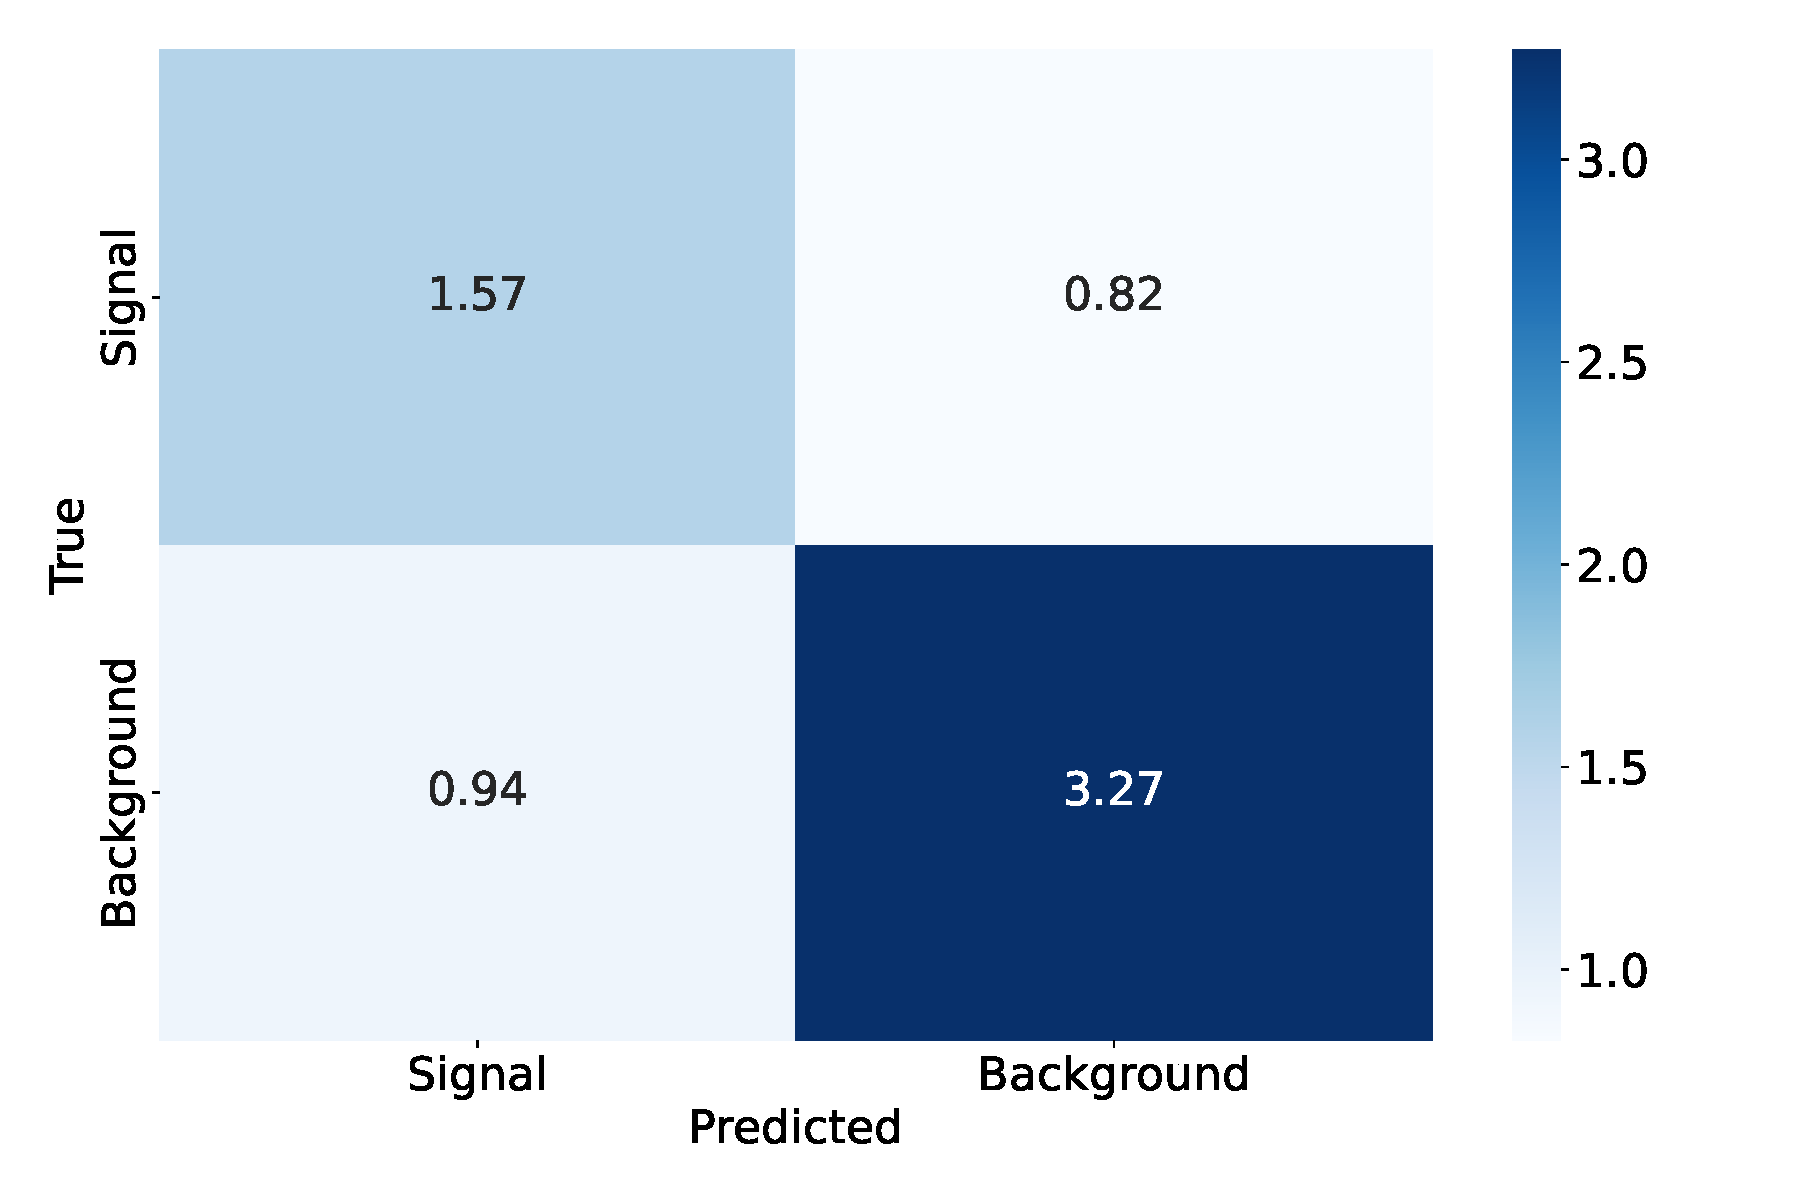
\includegraphics[trim=0.5cm 0 2cm 0, clip, width=0.8\textwidth]{figures/ml/cm/signal_argmax.pdf}
    \caption[Confusion matrix for a binary classification task]
    {Confusion matrix for a binary classification task. This confusion matrix is produced using 5-blocks
        \gls{ftt} (\autoref{sec:ftt}) trained on the extended training set (\autoref{sec:extended-set}) evaluated on the
        validation set, that contains 20\% of the \gls{sr} events. Signal refers to \tth, and background refers to all
        the other classes. The $\arg\max$ classification strategy was used.  Note that the classifier was \emph{trained}
        to differentiate between all the classes, but during evaluation, all the non-\tth events are grouped together.}
    \label{fig:cm}
\end{figure}

Binary confusion matrix naturally extends to a multi-class formulation (\autoref{fig:cm-muli}), leading to a
$|\classY| \times |\classY|$ matrix for a $|\classY|$-class classification task:

\begin{equation}
    \Cmulti_{ij} = \sum_{k=1}^{|\classY|} w_k \llbracket y_k = i \land \hat{y}_k = j \rrbracket\,,
\end{equation}

where $i$ and $j$ are the true and predicted classes, respectively. The diagonal elements of the matrix correspond to
the correctly classified events, while the off-diagonal elements correspond to the misclassified events. The
multi-class confusion matrix is not symmetric, and the sum of the elements in each row is equal to the number of events
in the corresponding true class.

\begin{figure}[htb]
    \centering
    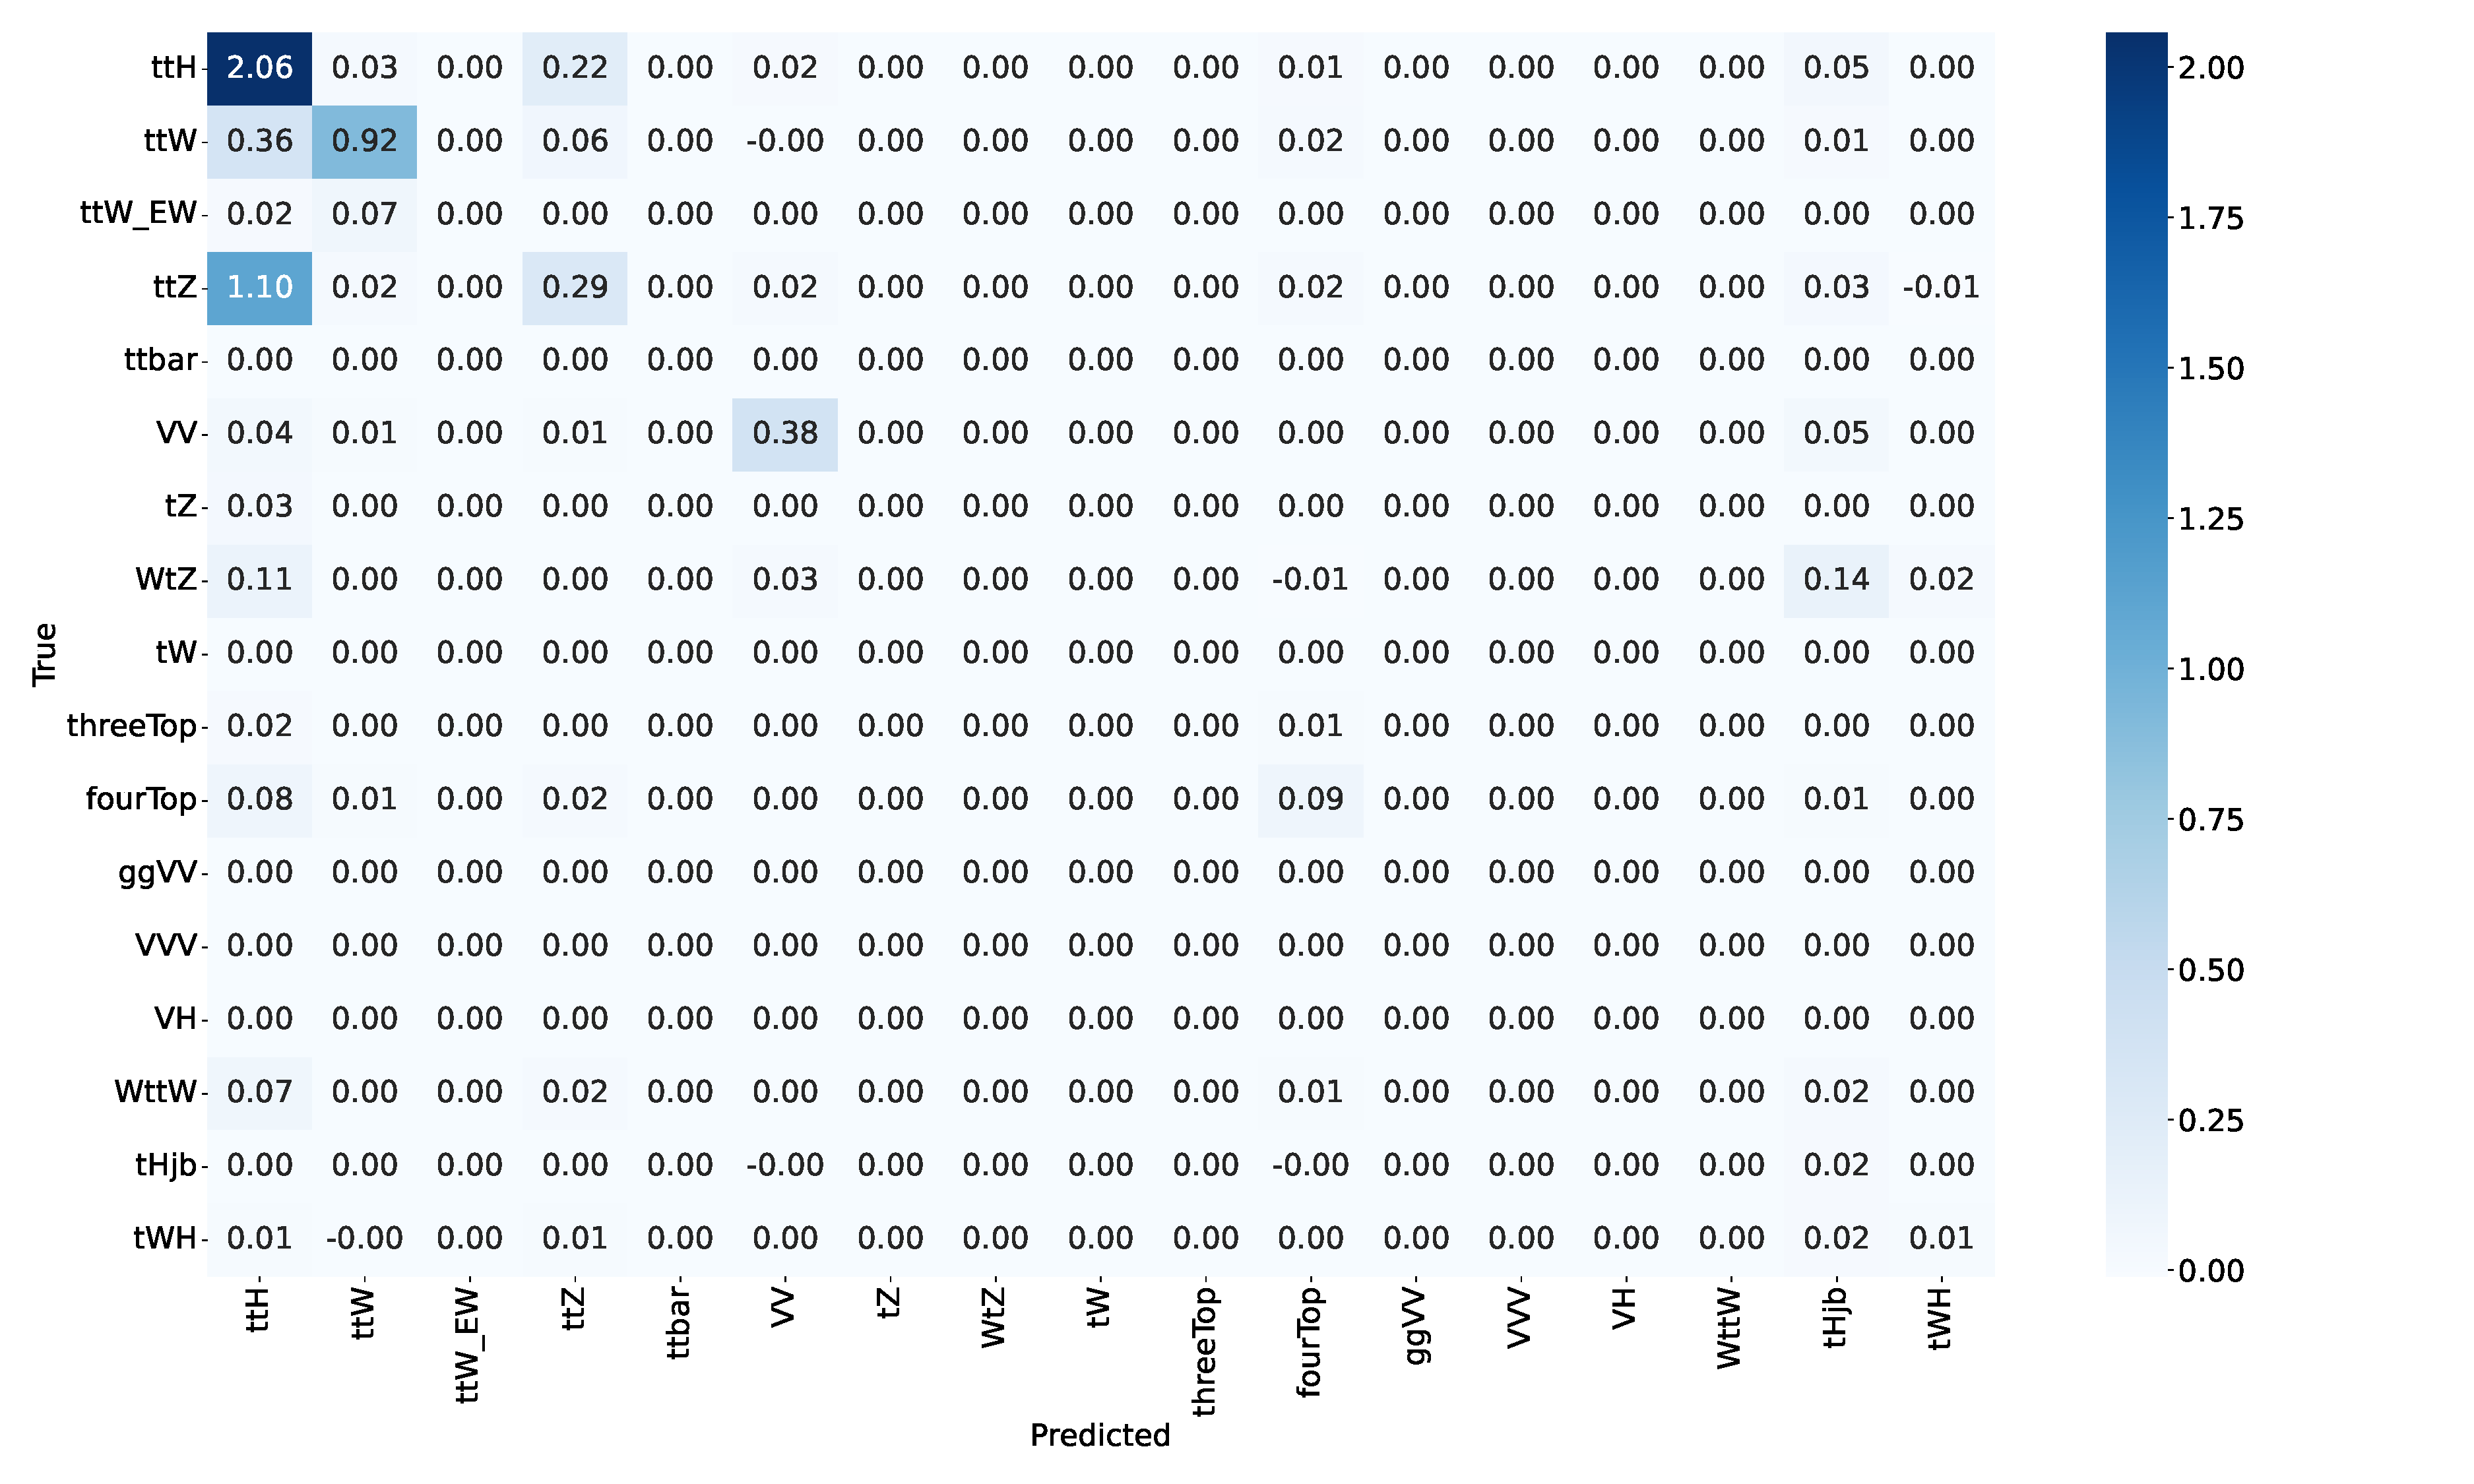
\includegraphics[trim=0.5cm 0 6cm 0, clip, width=\textwidth]{figures/ml/cm/all_argmax.pdf}
    \caption[Confusion matrix for a multi-class classification task]
    {Confusion matrix for a multi-class classification task. This confusion matrix is produced using 5-blocks
        \gls{ftt} (\autoref{sec:ftt}) trained on the extended training set (\autoref{sec:extended-set}). The
        $\arg\max$ classification strategy was used.}
    \label{fig:cm-muli}
\end{figure}

The confusion matrix serves as the basis for several other performance metrics, including accuracy, F1 score, and area
under the \gls{roc} curve (AUC-ROC).

\subsubsection{Accuracy: The Proportion of Correct Predictions}

Accuracy is the most intuitive performance metric. It is the ratio of the number of correctly classified examples
to the total number of examples (called events in particle physics). Accuracy is calculated trivially from the confusion
matrix:

\begin{align}
    \acc  = \frac{\trace \C_{ii}}{\sum_{i=1}^\classY \sum_{j=1}^\classY \C_{ij}}\,,
\end{align}

While accuracy is straightforward and commonly used, it may not always be the most representative metric, especially in
cases where the classes are imbalanced. Consider the example of our particle physics problem where we are searching for
\tth events and suppose that 90\% of the events are background and only 10\% are signal. A naïve classifier that
always predicts the background class would achieve an accuracy of 90\%. However, such a classifier would be entirely
unhelpful for the task at hand since it fails to identify any \tth events.

Certainly, the accuracy is not entirely without value, and there are contexts where it might still be useful. Even in
imbalanced scenarios, accuracy can provide a general sense of how often the classifier is correct across both the
majority and minority classes. While it may not provide a nuanced view of performance on the minority class (such as
\tth events in our case), it still provides information on the overall hit rate of correct predictions.

Additionally, in scenarios where the cost of false positives and false negatives are roughly equivalent, or when the
class distribution in the model's operational environment matches the training data, accuracy might still be a relevant
metric. It offers a quick and easily interpretable measure of performance.

However, in the specific context of searching for rare or significant events, such as \tth in particle physics, relying
solely on accuracy can be misleading. It would typically be considered alongside other metrics that give more insight
into the performance on the class of interest. Thus, while accuracy may not be the most representative metric in such
cases, it might still hold some value as part of a broader evaluation framework.

\subsubsection{Precision and Recall}

Two other important metrics which are derived from the confusion matrix are precision and recall, which are particularly
useful when dealing with imbalanced classes.

\paragraph{Precision} is the proportion of TP to all \emph{predicted} positives. Specifically, in our case, it is the
ratio of the correctly classified \tth events, to all events classified (or misclassified) as \tth. From here on, we
assume $y_1 = \tth$, and so the true \tth events correspond to the first row of the confusion matrix, while predicted
\tth events correspond to the first column. Precision is then given by

\begin{align}
    \text{Precision} = \frac{\C_{11}}{\sum_{j=1}^\classY \C_{1j}}\,.
\end{align}

\paragraph{Recall} (or sensitivity) is the proportion of TP to all \emph{actual} positives. In our case, it is the ratio
of the correctly classified \tth events to all actual \tth events (which the model might have missed by classifying them
as background). Recall is given by

\begin{align}
    \text{Recall} = \frac{\C_{11}}{\sum_{i=1}^\classY \C_{i1}}\,.
\end{align}

Precision tells us how reliable our positive predictions are,
while recall informs us how many of the actual \tth events we were able to detect. Both these metrics provide
complementary insights, and understanding the trade-off between them is essential in many real-world classification
tasks. Next, we will introduce the F1 score, a metric that combines both precision and recall to provide a balanced view
of the model's performance on both fronts.

\subsubsection{F1 Score: The Balance Between Precision and Recall}

The F1 score is the harmonic mean of precision and recall, providing a balance between the two. It is calculated as:

\begin{equation}
    \text{F1 score} = 2 \cdot \frac{\text{Precision} \cdot \text{Recall}}{\text{Precision} + \text{Recall}}
\end{equation}

\subsubsection{ROC Curve and AUC: The Trade-off Between Sensitivity and Specificity}

The \gls{roc} curve is a plot of the true positive rate (recall or sensitivity) against
the false positive rate (1 - specificity) for different classification thresholds. The area under the ROC curve
(AUC-ROC) measures the classifier's ability to distinguish between classes. A perfect classifier has an AUC-ROC of 1,
while a random classifier has an AUC-ROC of 0.5. The ROC curves for the \tth and two most dominant background processes
\ttw and \ttz are shown in \autoref{fig:rocs}.

\begin{figure}[htb]
    \centering
    \begin{subfigure}{0.32\textwidth}
        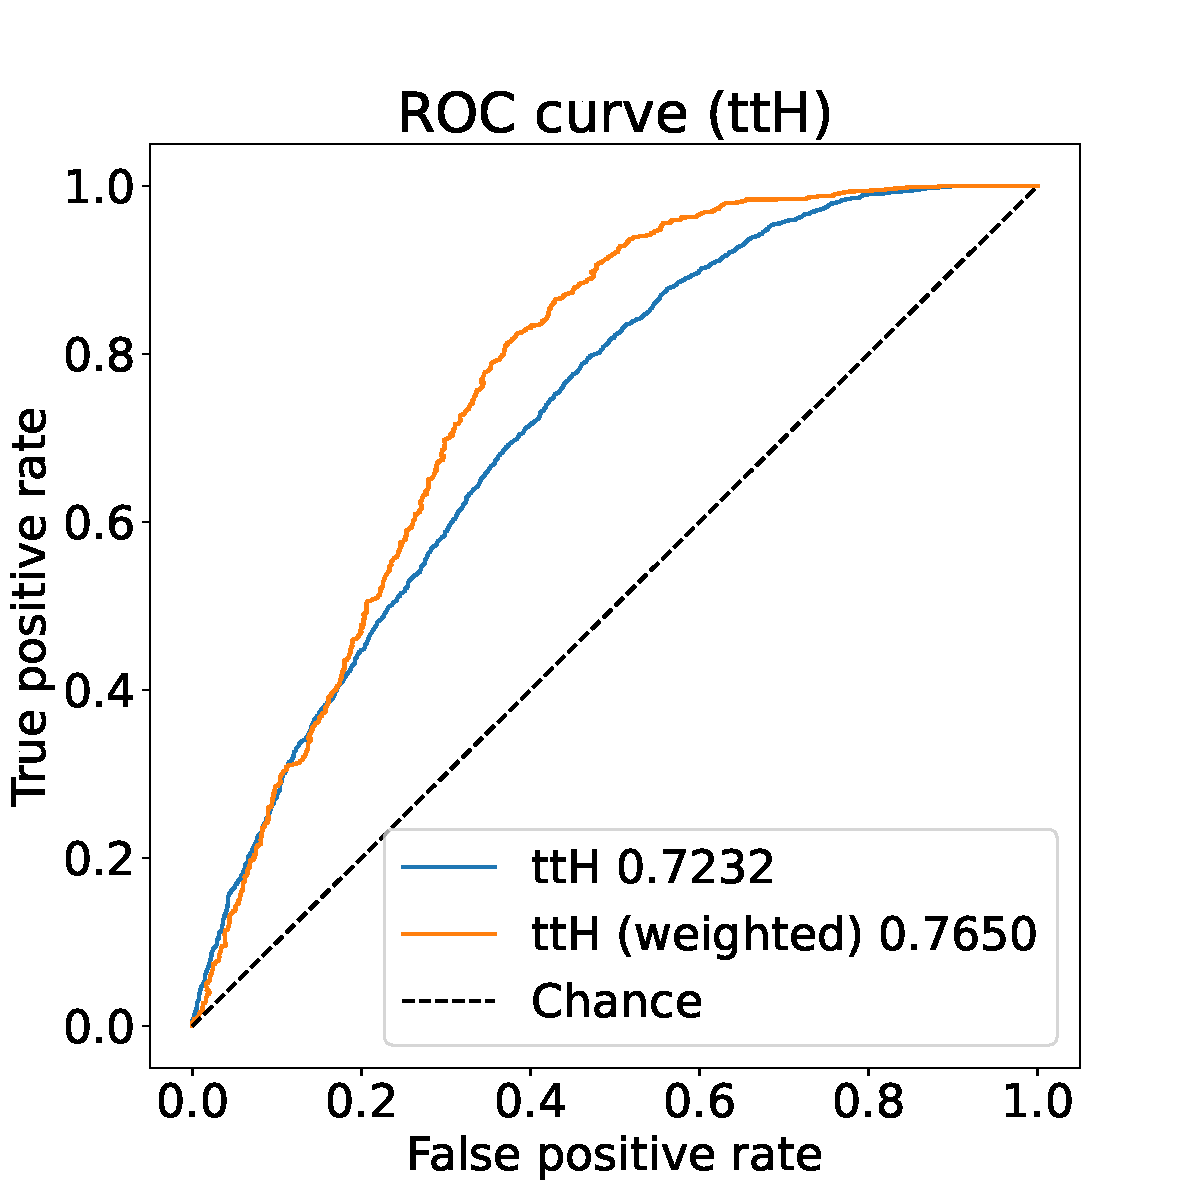
\includegraphics[width=\linewidth]{figures/ml/roc/ttH.pdf}
        \caption{\tth}
        \label{fig:roc-tth}
    \end{subfigure}
    \begin{subfigure}{0.32\textwidth}
        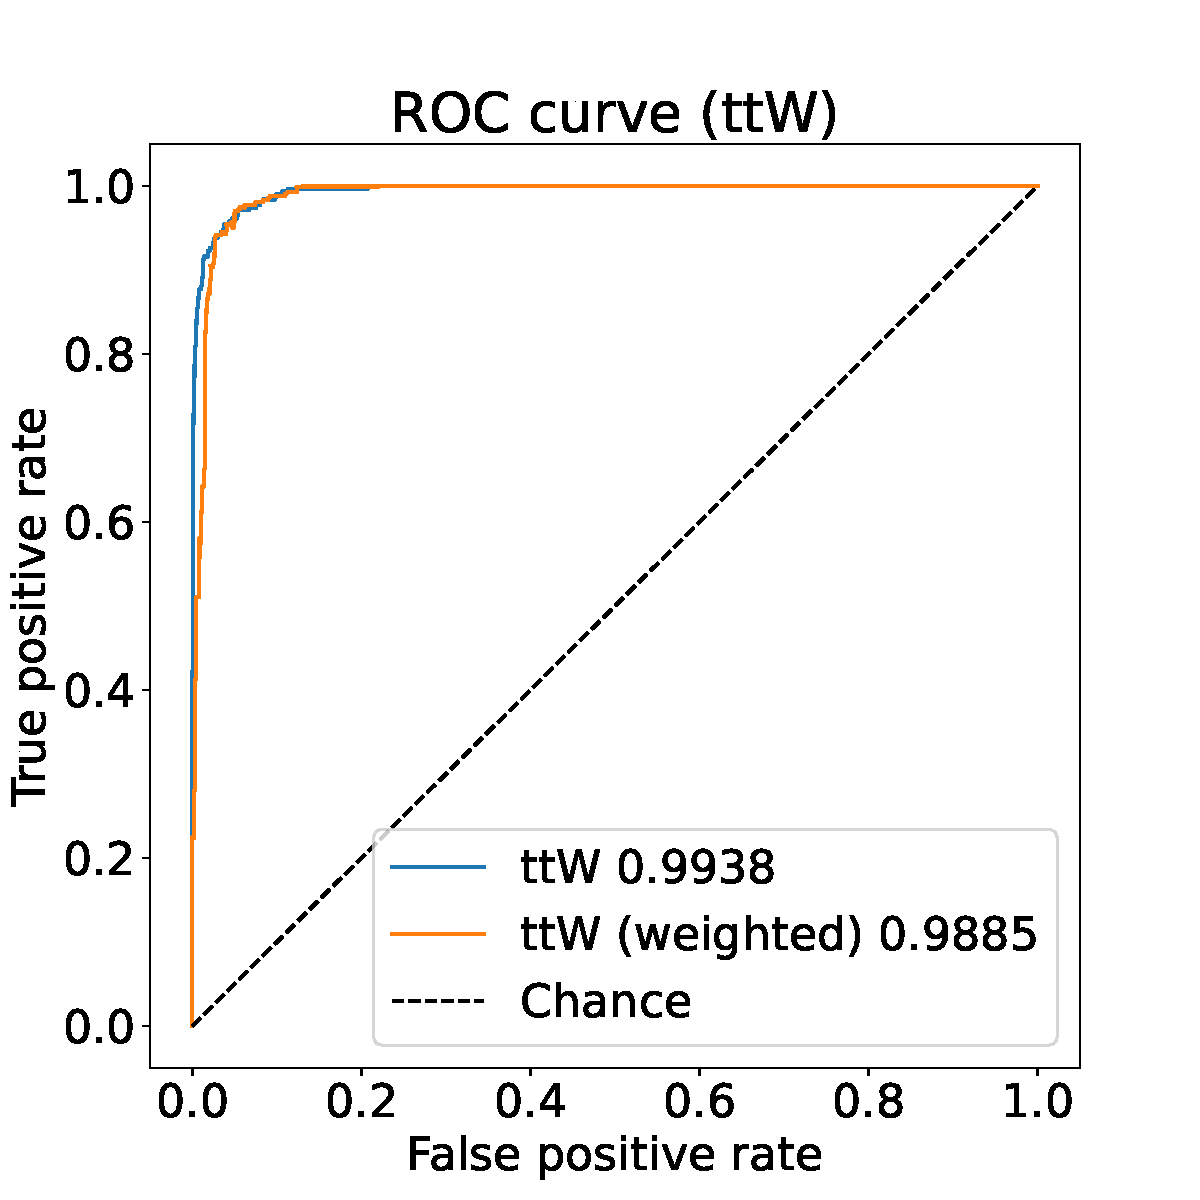
\includegraphics[width=\linewidth]{figures/ml/roc/ttW.pdf}
        \caption{\ttw}
        \label{fig:roc-ttw}
    \end{subfigure}
    \begin{subfigure}{0.32\textwidth}
        \includegraphics[width=\linewidth]{figures/ml/roc/ttZ.pdf}
        \caption{\ttz}
        \label{fig:roc-ttz}
    \end{subfigure}
    \caption[\acrshort{roc} curves for \tth, \ttz, and \ttz]
    {\gls{roc} curves for the \tth, \ttw, and \ttz computed using one process versus all other processes. The curves are produced
        using 5-blocks \gls{ftt} (\autoref{sec:ftt}) trained on the extended training set (\autoref{sec:extended-set}).
        We provide both the \glspl{roc} computed with the weighted and unweighted confusion matrices for completeness
        and comparison with the previous analysis, however, we emphasize that the weighted \glspl{roc} are the ones that
        should be used always.}
    \label{fig:rocs}
\end{figure}


These metrics, combined with the loss function, provide a comprehensive view of the classifier's performance and guide
the optimization process during training. They also provide a robust measure for comparing different classifiers or the
same classifier with different hyperparameters. Generally, one should examine all of these metrics to get a complete
picture of the classifier's performance.

% Include the architectures section
\section{V8 adaptation}

\section{\gls{sr} cut expression}
\label{appendix:cut-expression}

{\scriptsize
    \begin{verbatim}
    custTrigMatch_LooseID_FCLooseIso_DLT
    && (dilep_type && (lep_ID_0*lep_ID_1)>0)
    && ((lep_Pt_0 >= 10e3 && lep_Pt_1 >= 10e3) && (fabs(lep_Eta_0) <= 2.5 && fabs(lep_Eta_1) <= 2.5)
        && ((abs(lep_ID_0) == 13 && lep_isMedium_0 && lep_isolationLoose_VarRad_0 && passPLIVTight_0)
            || ((abs(lep_ID_0) == 11 && lep_isTightLH_0 && lep_isolationLoose_VarRad_0 && passPLIVTight_0
                && lep_ambiguityType_0 == 0 && lep_chargeIDBDTResult_recalc_rel207_tight_0 > 0.7)
                && ((!(!(lep_Mtrktrk_atConvV_CO_0 < 0.1 && lep_Mtrktrk_atConvV_CO_0 >= 0 && lep_RadiusCO_0 > 20)
                    && (lep_Mtrktrk_atPV_CO_0 < 0.1 && lep_Mtrktrk_atPV_CO_0 >= 0)))
                    && !(lep_Mtrktrk_atConvV_CO_0 <0.1 && lep_Mtrktrk_atConvV_CO_0 >= 0 && lep_RadiusCO_0 > 20))))
            && ((abs(lep_ID_1) == 13 && lep_isMedium_1 && lep_isolationLoose_VarRad_1 && passPLIVTight_1)
                || ((abs(lep_ID_1) == 11 && lep_isTightLH_1 && lep_isolationLoose_VarRad_1 && passPLIVTight_1
                    && lep_ambiguityType_1 == 0 && lep_chargeIDBDTResult_recalc_rel207_tight_1 > 0.7)
                    && ((!(!(lep_Mtrktrk_atConvV_CO_1 < 0.1 && lep_Mtrktrk_atConvV_CO_1 >= 0 && lep_RadiusCO_1 > 20)
                        && (lep_Mtrktrk_atPV_CO_1 < 0.1 && lep_Mtrktrk_atPV_CO_1 >= 0)))
                        && !(lep_Mtrktrk_atConvV_CO_1 < 0.1 && lep_Mtrktrk_atConvV_CO_1 >= 0 && lep_RadiusCO_1 > 20)))))
    && nTaus_OR==1
    && nJets_OR_DL1r_85>=1
    && nJets_OR>=4
    && ((dilep_type==2) || abs(Mll01-91.2e3)>10e3)
\end{verbatim}
}

We have kept the cuts the same as \cite{severin}, except for the cut on the \verb|nJets_OR| to \verb|>=4| to keep
consistent definition \gls{sr} definition across the group \todo{refer to the BDT group - how?}.

\section{Yields Plots}
\label{appendix:yields}

\begin{figure}[htb!]
    \centering
    \begin{subfigure}{0.45\textwidth}
        \includegraphics[width=\linewidth]{figures/yields/lep-pt-0.pdf}
        \caption{Distribution of the transverse momentum of the leading lepton.}
    \end{subfigure}\hfill%
    \begin{subfigure}{0.45\textwidth}
        \includegraphics[width=\linewidth]{figures/yields/lep-pt-1.pdf}
        \caption{Distribution of the transverse momentum of the subleading lepton.}
    \end{subfigure}
\end{figure}

\begin{figure}[htb!]
    \centering
    \begin{subfigure}{0.45\textwidth}
        \includegraphics[width=\linewidth]{figures/yields/n-jets.pdf}
        \caption{Distribution of the number of jets.}
    \end{subfigure}\hfill%
    \begin{subfigure}{0.45\textwidth}
        \includegraphics[width=\linewidth]{figures/yields/n-bjets.pdf}
        \caption{Distribution of the number of $b$-jets.}
    \end{subfigure}
\end{figure}

\begin{figure}[htb!]
    \centering
    \begin{subfigure}{0.45\textwidth}
        \includegraphics[width=\linewidth]{figures/yields/tau-width.pdf}
        \caption{Distribution of the $\tau$-jet width.}
    \end{subfigure}\hfill%
\end{figure}
\subsection{List of samples by each process}

The root directory for the files is:

{\small
\verb|/eos/atlas/atlascerngroupdisk/phys-higgs/HSG8/multilepton_ttWttH/v08/v0801/systematics-full/nominal|
}

The list of samples is given in \hyperref[tab:samples]{Table~\ref*{tab:samples}}.

\newpage

\begin{table}[h!]
    \centering
    \renewcommand{\arraystretch}{1.5}
    \caption{List of samples by each process}
    \label{tab:samples}
    \begin{tabular}{p{1.5cm}p{13.5cm}}
        \toprule
        Process      & \gls{dsid}                                                           \\
        \midrule
        $t\bar{t}H$  & p4498/346343, p4498/346344, p4498/346345                             \\
        $t\bar{t}W$  & p4416/700168, p4590/700205                                           \\
        $t\bar{t}Z$  & p4416/700168                                                         \\
        $t\bar{t}$   & p4308/410470                                                         \\
        $VV$         & \input{samples/VV.tex}                                               \\
        $ggVV$       & p4308/345705, p4396/345706, p4396/345715, p4396/345718, p4396/345723 \\
        $Zjets$      & \input{samples/Zjets.tex}                                            \\
        $Wjets$      & \input{samples/Wjets.tex}                                            \\
        $tW$         & p4308/410646, p4308/410647                                           \\
        $threeTop$   & p4308/304014                                                         \\
        $fourTop$    & p4308/410080                                                         \\
        $t\bar{t}WW$ & p4308/410081                                                         \\
        $tZ$         & p4308/410560                                                         \\
        $WtZ$        & p4308/410408                                                         \\
        $VVV$        & \input{samples/VVV.tex}                                              \\
        $VH$         & p4308/342284, p4308/342285                                           \\
        $tHjb$       & p4308/346799\_AF                                                     \\
        $tWH$        & p4308/346678\_AF                                                     \\
        \bottomrule
    \end{tabular}
\end{table}

\newpage
\subsection{Distribution of the variables inside \gls{sr}}

The following figures (\autoref{fig:distributions1} and \autoref{fig:distributions2}) show the distributions of some variables
of interest inside \gls{sr}.

\captionsetup[subfigure]{justification=centering}
\begin{figure}[htb!]
    \centering
    \begin{subfigure}{0.45\textwidth}
        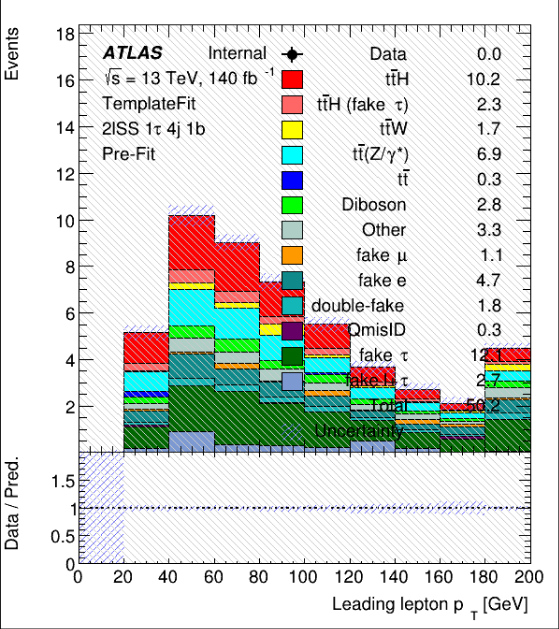
\includegraphics[width=\linewidth]{figures/plots/histograms/lep_pt_0.png}
        \caption{Distribution of the transverse momentum of the leading lepton.}
        \label{fig:lep_pt_0}
    \end{subfigure}\hfill%
    \begin{subfigure}{0.45\textwidth}
        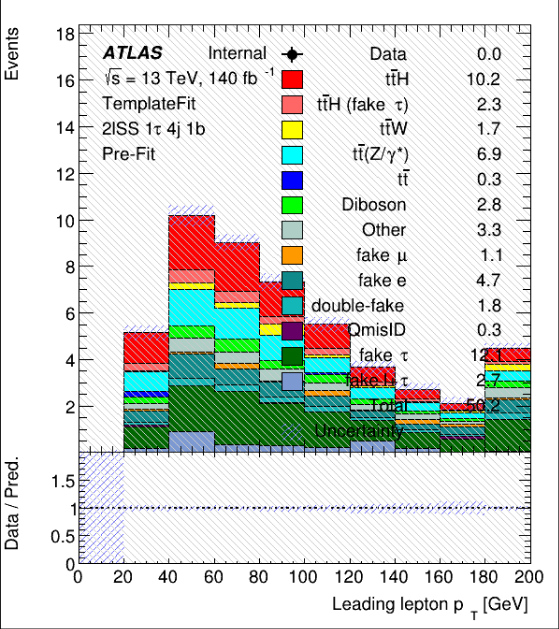
\includegraphics[width=\linewidth]{figures/plots/histograms/lep_pt_1.png}
        \caption{Distribution of the transverse momentum of the subleading lepton.}
        \label{fig:lep_pt_1}
    \end{subfigure}

    \vspace{0.5cm}

    \begin{subfigure}{0.45\textwidth}
        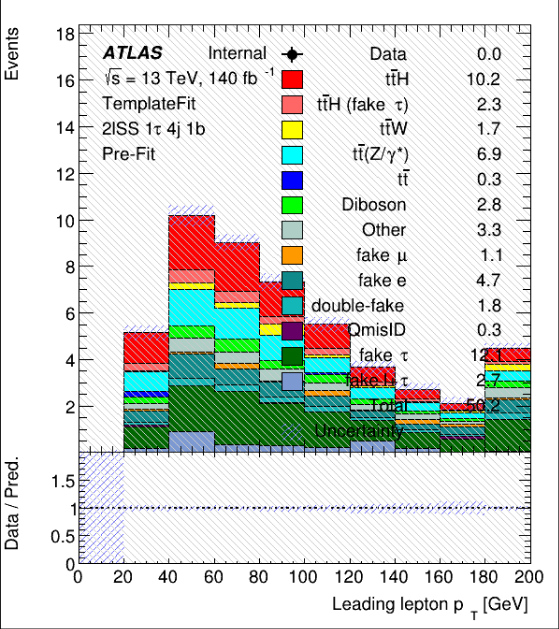
\includegraphics[width=\linewidth]{figures/plots/histograms/lep_Eta_0.png}
        \caption{Distribution of the pseudorapidity of the leading lepton.}
        \label{fig:lep_Eta_0}
    \end{subfigure}\hfill%
    \begin{subfigure}{0.45\textwidth}
        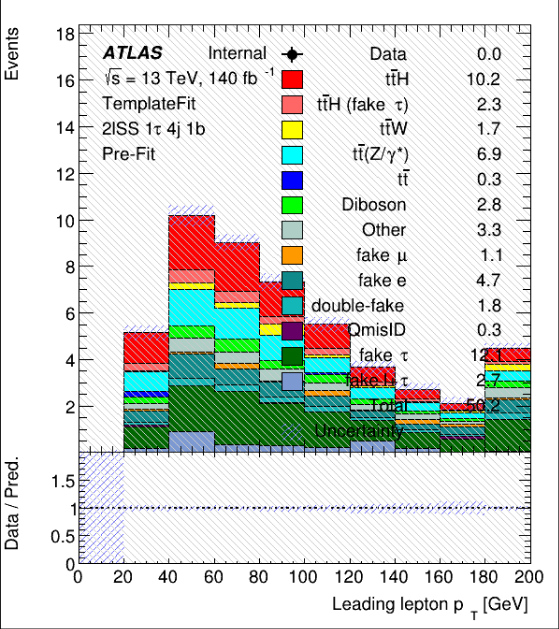
\includegraphics[width=\linewidth]{figures/plots/histograms/lep_Eta_1.png}
        \caption{Distribution of the pseudorapidity of the subleading lepton.}
        \label{fig:lep_Eta_1}
    \end{subfigure}
    \caption{Distributions of the variables inside \gls{sr} (part 1)}
    \label{fig:distributions1}
\end{figure}

\newpage

\begin{figure}[htb!]
    \centering
    \begin{subfigure}{0.45\textwidth}
        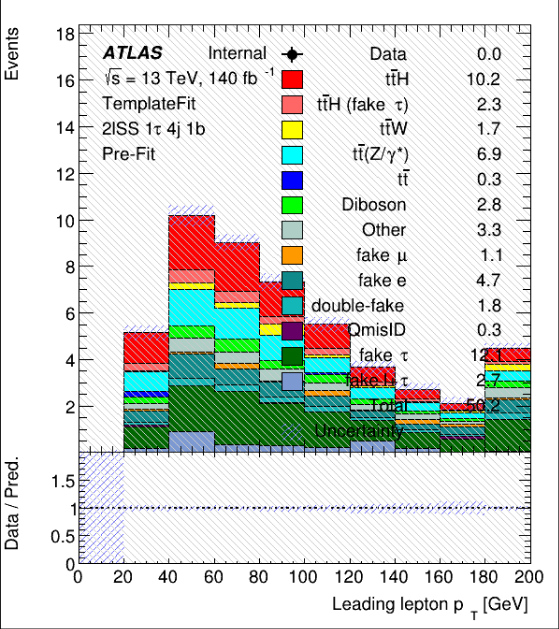
\includegraphics[width=\linewidth]{figures/plots/histograms/lep_Phi_0.png}
        \caption{Distribution of the azimuthal angle of the leading lepton.}
        \label{fig:lep_Phi_0}
    \end{subfigure}\hfill%
    \begin{subfigure}{0.45\textwidth}
        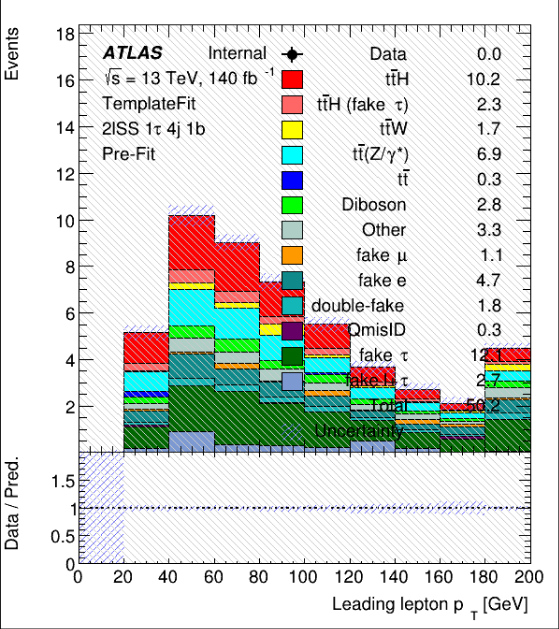
\includegraphics[width=\linewidth]{figures/plots/histograms/lep_Phi_1.png}
        \caption{Distribution of the azimuthal angle of the subleading lepton.}
        \label{fig:lep_Phi_1}
    \end{subfigure}

    \vspace{0.5cm}

    \begin{subfigure}{0.45\textwidth}
        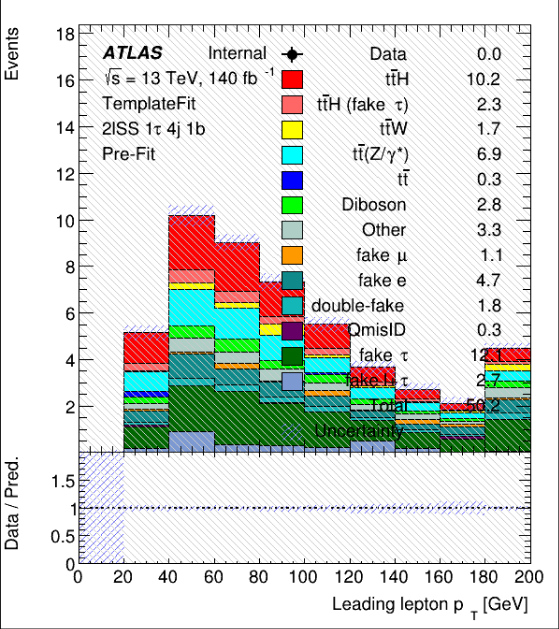
\includegraphics[width=\linewidth]{figures/plots/histograms/njets.png}
        \caption{Distribution of the number of jets.}
        \label{fig:njets}
    \end{subfigure}\hfill%
    \begin{subfigure}{0.45\textwidth}
        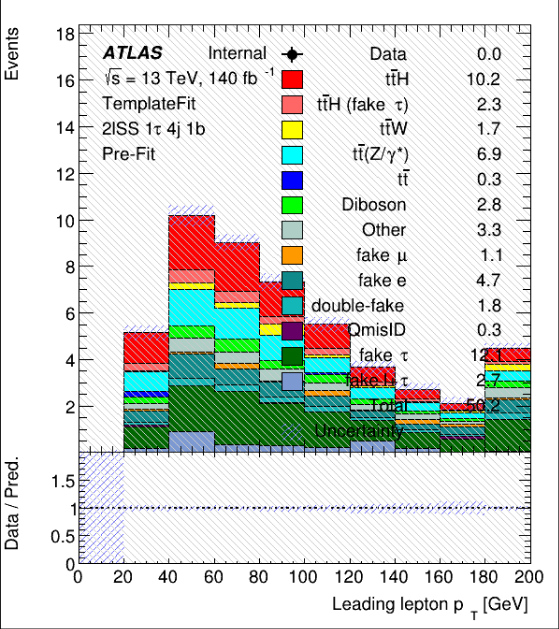
\includegraphics[width=\linewidth]{figures/plots/histograms/nbjets.png}
        \caption{Distribution of the number of $b$-jets.}
        \label{fig:nbjets}
    \end{subfigure}
    \caption{Distributions of the variables inside \gls{sr} (part 2)}
    \label{fig:distributions2}
\end{figure}

\begin{minipage}{0.45\textwidth}
    \centering
    \begin{tabular}{c|c|c|c|c}
        $t\bar{t}H$ & \textbf{v6} & \textbf{v8} &      &       \\
        \hline
        Weighted    & 1000        & 500         & -500 & -50\% \\
        Raw         & 1000        & 500         & -500 & -50\% \\
        \hline
    \end{tabular}
    \captionof{table}{Number of ttH events in the SR for v6 and v8.}
    \label{tab:ttH_event_numbers1}
\end{minipage}\hfill%
\begin{minipage}{0.45\textwidth}
    \centering
    \begin{tabular}{c|c|c|c|c}
        \gls{sr} & \textbf{v6} & \textbf{v8} &      &       \\
        \hline
        Weighted & 1000        & 500         & -500 & -50\% \\
        Raw      & 1000        & 500         & -500 & -50\% \\
        \hline
    \end{tabular}
    \captionof{table}{Number of all the events in the SR for v6 and v8.}
    \label{tab:ttH_event_numbers2}
\end{minipage}

\clearpage \subsection{Features used}

\subsubsection{\texttt{lep\_E\_X}} The energy of the Xth lepton.

\subsubsection{\texttt{DRjj\_lead}} $\Delta R$ between the two leading jets. $\Delta R$ is a distance metric in the
$\eta-\phi$ space frequently used in particle physics.

\subsubsection{\texttt{Ptll01}} The transverse momentum of the dilepton system made up of the two leading leptons.

\subsubsection{\texttt{lep\_nTrackParticles\_X}} The number of track particles associated with the Xth lepton.

\subsubsection{\texttt{custTrigMatch\_LooseID\_FCLooseIso\_DLT}} Custom trigger matching for loosely identified and loosely
isolated leptons, likely related to the dilepton trigger

\subsubsection{\texttt{Mll01}} The invariant mass of the two leading leptons.

\subsubsection{\texttt{Mlll012}} The invariant mass of the three leading leptons.

\subsubsection{\texttt{total\_charge}} The sum of the electric charges of the particles in the event.

\subsubsection{\texttt{HT}} The scalar sum of the transverse momenta of all jets in the event.

\subsubsection{\texttt{HT\_lep}} The scalar sum of the transverse momenta of all leptons in the event.

\subsubsection{\texttt{lep\_Eta\_X}} The pseudorapidity of the Xth lepton.

\subsubsection{\texttt{nTaus\_OR\_Pt25}} The number of overlapping-removed taus with a transverse momentum above 25 GeV.

\subsubsection{\texttt{nFwdJets\_OR}} The number of overlapping-removed forward jets.

\subsubsection{\texttt{MLepMet}} The invariant mass of a lepton and the missing transverse energy vector.

\subsubsection{\texttt{taus\_DL1r\_X}} The DL1r score for the Xth tau.

\subsubsection{\texttt{lep\_isolationLoose\_VarRad\_X}} Indicates whether a lepton (where X refers to the lepton index)
passes an isolation cut with a variable radius. Looser isolation cuts allow more nearby activity in the detector.

\subsubsection{\texttt{lep\_EtaBE2\_X}} The pseudorapidity of the Xth lepton in the second layer of the electromagnetic
calorimeter.

\subsubsection{\texttt{HT\_fwdJets}} The scalar sum of the transverse momenta of all forward jets in the event.

\subsubsection{\texttt{taus\_width\_X}} The width of the Xth tau.

\subsubsection{\texttt{nJets\_OR\_DL1r\_85}} Count of jets that pass overlap removal (OR) and are b-tagged according to the
DL1r algorithm at the 85\% working point.

\subsubsection{\texttt{lep\_nInnerPix\_X}} Number of hits in the inner pixel detector associated with the lepton, where X
refers to the lepton index.

\subsubsection{\texttt{met\_phi}} The azimuthal angle of the missing transverse energy in the event.

\subsubsection{\texttt{DeltaR\_max\_lep\_bjet77}} The maximum DeltaR value between a lepton and a b-tagged jet. The "77"
may refer to the working point of the b-tagging algorithm.

\subsubsection{\texttt{MbX}} Invariant mass associated with the leading b-jet in the event

\subsubsection{\texttt{lep\_RadiusCO\_X}} Possibly the radius of the cone used for isolation of the lepton, or
alternatively a parameter associated with the trajectory of the lepton.

\subsubsection{\texttt{lep\_Mtrktrk\_atConvV\_CO\_X}} The invariant mass of track pairs at the conversion vertex for lepton
X. This might be related to photon conversions into an electron-positron pair.

\subsubsection{\texttt{lep\_Z0SinTheta\_X}} The z0 impact parameter times the sine of the lepton's polar angle.

\subsubsection{\texttt{lep\_Pt\_X}} The transverse momentum of the Xth lepton.

\subsubsection{\texttt{mjjMax\_frwdJet}} The maximum invariant mass of a pair of forward jets.

\subsubsection{\texttt{dilep\_type}} The type of dilepton event (e.g., $ee$, $\mu e$, $\mu \mu$).

\subsubsection{\texttt{eta\_frwdjet}} The pseudorapidity of the forward jet.

\subsubsection{\texttt{Mlb}} Invariant mass of a lepton and a b-jet.

\subsubsection{\texttt{taus\_RNNJetScoreSigTrans\_X}} Transformed RNN-based score for tau lepton, possibly to better
separate signal from background.

\subsubsection{\texttt{minDeltaR\_LJ\_X}} The minimum $\Delta R$ distance between the Xth lepton and any jet in the event.

\subsubsection{\texttt{nTaus\_OR}} Number of tau leptons that pass overlap removal. Overlap removal is a step in particle
reconstruction where, for instance, an object identified as both a jet and a tau would be considered only as one or the
other.

\subsubsection{\texttt{DeltaR\_min\_lep\_jet}} The minimum $\Delta R$ distance between a lepton and a jet in the event.

\subsubsection{\texttt{lep\_sigd0PV\_X}} Significance of the transverse impact parameter (d0) of the lepton X with respect
to the primary vertex (PV). This is a common variable for distinguishing prompt particles produced in the primary
collision from secondary particles produced in a decay.

\subsubsection{\texttt{taus\_eta\_X}} The pseudorapidity of the Xth tau.

\subsubsection{\texttt{HT\_jets}} The scalar sum of the transverse momenta of all jets (not forward jets) in the event.

\subsubsection{\texttt{lep\_Phi\_X}} The azimuthal angle (in radians) of the Xth lepton.

\subsubsection{\texttt{bTagSF\_weight\_DL1r\_85}} A weight applied to events based on the scale factor for b-tagging using
the DL1r algorithm at an 85\% efficiency working point. This scale factor corrects the b-tagging efficiency in Monte
Carlo simulations to match that observed in real data.

\subsubsection{\texttt{lep\_chargeIDBDTResult\_recalc\_rel207\_tight\_X}} The outcome of a BDT-based charge identification
for a lepton, recalculated with some specific settings, and applying a 'tight' threshold.

\subsubsection{\texttt{taus\_phi\_X}} The azimuthal angle (in radians) of the Xth tau.

\subsubsection{\texttt{taus\_passJVT\_X}} A boolean flag indicating whether the Xth tau passes the jet vertex tightness
(JVT) requirement.

\subsubsection{\texttt{jets\_eta}} The pseudorapidity of the jets (array).

\subsubsection{\texttt{taus\_charge\_X}} The charge of the Xth tau.

\subsubsection{\texttt{passPLIVTight\_X}} Boolean flag indicating if a lepton with high transverse momentum passes the
"tight" criteria of the Prompt Lepton Veto (PLIV), a tool for identifying non-prompt light leptons.

\subsubsection{\texttt{lep\_Mtrktrk\_atPV\_CO\_X}} The invariant mass of track pairs at the primary vertex for lepton X.
This could be related to certain types of particle decays happening at the primary collision vertex.

\subsubsection{\texttt{taus\_JetRNNSigMedium\_X}} RNN-based score for tau lepton, used to distinguish tau leptons from
jets, with 'medium' selection criteria.

\subsubsection{\texttt{minOSMll}} The minimum invariant mass of oppositely-signed dilepton pairs.

\subsubsection{\texttt{lep\_ID\_X}} The identification number for the Xth lepton.

\subsubsection{\texttt{Mllll0123}} The invariant mass of the four leading leptons.

\subsubsection{\texttt{custTrigSF\_TightElMediumMuID\_FCLooseIso\_DLT}} Custom trigger scale factor, for events with a
tight electron and a medium muon, both of which are loosely isolated, likely related to the dilepton trigger (DLT).

\subsubsection{\texttt{best\_Z\_Mll}} The invariant mass of the dilepton system that is closest to the Z boson mass.

\subsubsection{\texttt{met\_met}} The missing transverse energy in the event.

\subsubsection{\texttt{MtLep1Met}} Transverse mass between the leading lepton and missing transverse energy. Transverse
mass is often used in searches for particles that decay to a lepton and a neutrino.

\subsubsection{\texttt{lep\_ambiguityType\_X}} Type of ambiguity for lepton identification, where X refers to the lepton
index. Ambiguity could arise from several factors, such as a single track matching with multiple reconstructed
particles.

\subsubsection{\texttt{jets\_phi}} The azimuthal angle (in radians) of the jets (array).

\subsubsection{\texttt{lep\_isMedium\_X}} Boolean flag indicating if a lepton passes the 'medium' selection criteria.

\subsubsection{\texttt{taus\_RNNJetScore\_X}} RNN-based score for tau lepton, used to distinguish tau leptons from jets.

\subsubsection{\texttt{MtLepMet}} The transverse mass of a lepton and the missing transverse energy vector.

\subsubsection{\texttt{DeltaR\_min\_lep\_jet\_fwd}} The minimum $\Delta R$ distance between a lepton and a forward jet in the event.

\subsubsection{\texttt{jets\_e}} The energy of the jets (array).

\subsubsection{\texttt{minOSSFMll}} The minimum invariant mass of oppositely-signed, same-flavor dilepton pairs.

\subsubsection{\texttt{nJets\_OR}} The number of overlapping-removed jets.

\subsubsection{\texttt{total\_leptons}} The total number of leptons in the event.

\subsubsection{\texttt{taus\_numTrack\_X}} The number of tracks associated with the Xth tau.

\subsubsection{\texttt{HT\_taus}} Scalar sum of the transverse momenta ($P_t$) of all tau leptons in the event.

\subsubsection{\texttt{taus\_passEleOLR\_X}} A boolean flag indicating whether the Xth tau passes the electron overlap
removal.

\subsubsection{\texttt{HT\_inclFwdJets}} The scalar sum of the transverse momenta of all jets, including forward jets, in
the event.

\subsubsection{\texttt{DRll01}} The $\Delta R$ distance between the two leading leptons.

\subsubsection{\texttt{taus\_JetRNNSigLoose\_X}} RNN-based score for tau lepton, used to distinguish tau leptons from
jets, with 'loose' selection criteria.

\subsubsection{\texttt{taus\_pt\_X}} The transverse momentum of the Xth tau.

\subsubsection{\texttt{bTagSF\_weight\_DL1r\_77}} A weight applied to events based on the scale factor for b-tagging using
the DL1r algorithm at an 77\% efficiency working point. This scale factor corrects the b-tagging efficiency in Monte
Carlo simulations to match that observed in real data.

\subsubsection{\texttt{flag\_JetCleaning\_LooseBad}} A flag variable indicating whether a jet passes a loose cleaning cut
to remove bad or noisy jets from the analysis.

\subsubsection{\texttt{taus\_fromPV\_X}} A boolean flag indicating whether the Xth tau comes from the primary vertex.

\subsubsection{\texttt{best\_Z\_other\_MtLepMet}} The transverse mass between the lepton and missing transverse energy for
the event that best reconstructs a Z boson using other criteria.

\subsubsection{\texttt{nJets\_OR\_DL1r\_77}} Count of jets that pass overlap removal (OR) and are b-tagged according to the
DL1r algorithm at the 77\% working point.

\subsubsection{\texttt{jets\_pt}} The transverse momentum of the jets (array).

\subsubsection{\texttt{lep\_isTightLH\_X}} Boolean flag indicating if a lepton passes the 'tight' Likelihood-based
identification criteria.

\subsubsection{\texttt{taus\_JetRNNSigTight\_X}} RNN-based score for tau lepton, used to distinguish tau leptons from
jets, with 'tight' selection criteria.

\subsubsection{\texttt{sumPsbtag}} The sum of b-tagging weights for jets in the event.

\subsubsection{\texttt{taus\_decayMode\_X}} The decay mode of the Xth tau.

\subsubsection{\texttt{dEta\_maxMjj\_frwdjet}} The maximum difference in pseudorapidity ($\eta$) between two forward jets.

\subsubsection{\texttt{max\_eta}} The maximum pseudorapidity among all particles in the event.

\subsubsection{\texttt{best\_Z\_other\_Mll}} The invariant mass of the dilepton system that is closest to the Z boson mass,
not considering the leading leptons.

\subsubsection{\texttt{taus\_passEleBDT\_X}} Flag indicating if a tau lepton passes the Electron Boosted Decision Tree
discriminator.

\begin{figure}[hbtp]
    \centering
    \includegraphics[width=\textwidth]{figures/ml/features/top20.pdf}
    \caption{Feature importance for the top 20 most important features. Feature importance was calculated using the
        \gls{ig} method \cite{ig}.}
    \label{fig:feature_importance}
\end{figure}

\clearpage

% Generate the results figure
\begin{figure}
    \centering
    \includegraphics{example-image-a}
    \caption{Results of all the notable techniques \todo{todo}}
    \label{tab:results}
\end{figure}

% This chapter describes the methodology used in this study. It includes the formulation of the problem, the evaluation metrics used, and the architectures tested.
\chapter{Methodology}
\label{ch:Methodology}

% Include the formulation section
\section{Problem Formulation}
\label{sec:formulation}

\todo{proofread}

\glsreset{erm}
\subsection[Empirical Risk Minimization]{\gls{erm}}

As stated before, our primary objective in this thesis is to distinguish the \tth events from other events of the other
detected by the \gls{atlas} detector. Given an observation $\bm{x} \in \mathcal{X}$, we want to predict its
corresponding class label $y \in \mathcal{Y}$. Here $\mathcal{X}$ denotes the space of all possible observations (in
our case this corresponds to the different measurements of the event), and $\mathcal{Y}$ denotes the space of all
the class labels we are differentiating between. We can further split the problem into either a binary classification
(seeking to differentiate between \tth (signal) and not \tth (background)) or a multi-class classification (seeking to
correctly discriminate between each of the processes - \tth, \ttw, \ttz, \ttbar, etc.).

As we approach this task as a supervised learning problem (recall \autoref{sec:mc}), we assume that a set of labeled
observations $\ttrn = {(\bm{x}_i, y_i)}_{i=1}^N$ is provided.  Here $\bm{x}_i \in \mathbf{X}$ is a feature vector
representing different properties (features) of an event and $y_i \in \mathbf{Y}$ is its corresponding true class label.
We assume there exists a joint probability distribution $P(\bm{x}, y)$ over the observations $\bm{x}$ and their
corresponding class labels $y$. Then, we require the examples in the training set $(\bm{x}_i, y_i) \in \ttrn$ to be
drawn \gls{iid} from the joint distribution $P(\bm{x}, y)$.


We also assume that there is a non-negative real-valued loss function $L(y, \hat{y})$ that quantifies the
discrepancy between the true label $y$ and the predicted label $\hat{y}$. The common example of such a loss function
would be a zero-one loss function, which is defined as

\begin{equation}
    L_{0/1}(y, \hat{y}) = \begin{cases}
        0 & \text{if } y = \hat{y} \\
        1 & \text{otherwise}
    \end{cases}\,.
\end{equation}

The goal is to find the best hypothesis $h^* \in \mathcal{H}:
    \mathbf{X} \rightarrow \mathbf{Y}$ that would minimize the expected loss over the joint distribution $P(\bm{x}, y)$:

\begin{equation}
    h^* = \argmin_{h \in \mathcal{H}} \mathbb{E}_{(\bm{x}, y) \sim P(\bm{x}, y)}[L(y, h(\bm{x}))]\,.
\end{equation}

In practice, we do not have access to the joint distribution $P(\bm{x}, y)$, but only to the training set $\ttrn$. To
tackle this problem, we use the \gls{erm} principle \cite{risk-minimization}, which states that the best hypothesis
$h^*$ is the one that minimizes the empirical risk over the training set $\ttrn$:

\begin{equation}
    \hat{h} = \argmin_{h \in \mathcal{H}} R_\ttrn(h) = \argmin_{h \in \mathcal{H}} \frac{1}{N} \sum_{i=1}^{N} L(y_i, h(\bm{x}_i))\,.
\end{equation}










\subsection{Validation and Test Sets}

Consider, for example the following "cheating" classifier:

\begin{equation}
    h(\bm{x}) = \begin{cases}
        y_i & \text{if } \exists i : \bm{x} = \bm{x}_i \\
        y_0 & \text{otherwise}
    \end{cases}\,.
\end{equation}


This classifier would have zero empirical risk, but would perform poorly on unseen data (would not generalize well).
This is referred to as overfitting (see \autoref{fig:standard-losses}). Generally, in case of an unconstrained
hypothesis space $\mathcal{H}$, we have no guarantee that the empirical risk $R_\ttrn(h)$ is a good approximation of the
true risk $R(h)$.


Specifically, the problem in this case is that the prediction $\hat{y}_i$ depends not only on the observation
$\bm{x}_i$, but also on the labels $y_1, \dots, y_N$. Consider, for example, a \gls{nn} classifier $h_\nnparams$ with trainable
parameters $\nnparams$. When training $h_\nnparams$ on the training set by back-propagation, $\nnparams$  becomes implicitly
conditioned on the true labels $y^1, \dots, y^s$ that the network has encountered before ($s$ denotes the training step).
This violates the \gls{iid} assumption and thus the empirical risk $R_\ttrn(h_\nnparams)$ is not a good approximation of
the true risk $R(h_\nnparams)$ anymore.


To address this issue and more accurately assess the generalization ability of the classifier $h$, We would need a
separate set $\tval \sim P(\bm{x}, y)$ that would provide an unbiased estimate of the true risk $R(h)$. This set is
called the validation set. Validation set is used to compare the performance of different
classifiers. Consider two classifiers $h_1$ and $h_2$, where the risk on the training set is $R_\ttrn(h_1) <
    R_\ttrn(h_2)$, but the risk on the validation set is $R_\tval(h_1) > R_\tval(h_2)$. In this case, we would prefer the
classifier $h_2$ over $h_1$ as it generalizes better to unseen data. The specific case is often seen with the \gls{nn}
classifiers, where the classifier $h$ is parametrized by $\nnparams$. Then essentially we compare $h_1 = h_{\nnparams_1}$ and
$h_2 = h_{\nnparams_2}$, where $\nnparams_1$ and $\nnparams_2$ are two different sets of parameters. The process of selecting
the best classifier $h^*$ from a set of classifiers $\mathcal{H}$ is called model selection.

\begin{figure}[htb]
    \centering
    \begin{minipage}[t][\height][t]{0.47\textwidth}
        \includegraphics[width=\textwidth]{figures/ml/training/standard-ts-losses.png}
        \caption{\acrshort{ftt} with 2 blocks and 256 embedding size training on the standard training set.}
        \label{fig:standard-losses}
    \end{minipage}
    \hfill
    \begin{minipage}[t][\height][t]{0.47\textwidth}
        \includegraphics[width=\textwidth]{figures/ml/training/extended-ts-losses.png}
        \caption{\acrshort{ftt} with 5 blocks, 256 embedding size, and 20\% dropout training on the \emph{extended} training
            set.} \label{fig:extended-losses}
    \end{minipage}
    \caption[Training and validation losses during the training process with and without extended training set.]
    {Training and validation losses during the training process with and without extended training set.
        \autoref{fig:standard-losses} shows the training of the \acrshort{ftt} with 2 blocks (see \autoref{sec:ftt}) on the
        standard training set. Because of the lack of training samples, and high capacity of the model, we observe
        overfitting. The training loss continues to decrease while the validation loss starts to increase. The
        checkpoint with the validation loss is the lowest is then used as the final model. This is referred to as early
        stopping. The best way to prevent overfitting is to get more training data (see
        \autoref{sec:extended-set}). If that is not possible, one might also consider augmentation techniques, or
        regularization - dropout (see \autoref{sec:dropout}), weight decay etc. \autoref{fig:extended-losses} shows the
        training of the \acrshort{ftt} with 5 blocks (see \autoref{sec:ftt}) on the extended training set. Also, the 20\%
        dropout is introduced. We observe now only a slight overfitting, which means that the model has generalized
        a lot better.}
    \label{fig:losses}
\end{figure}

The caveat of using the validation for model selection is that in doing so we are implicitly fitting to the validation set,
as now our best classifier $h^*$ is also conditioned on the evaluations of the other classifiers on the validation set.
To address the similar issue, a third set is normally introduced, called the test set $\ttst \sim P(\bm{x}, y)$. The test
set should be used only once to assess the performance of the fully-trained classifier $h^*$.




\todo{But then why we don't use the test set in our thesis???}





\subsection{Training}

The process of finding the best hypothesis $h^*$ is called training (or learning). In the context of \gls{erm}, this
further reduces to minimization of the empirical risk $R_\ttrn(h)$. As described before, the empirical risk is an
expectation of the loss function $L(y, h(\bm{x}))$ over the training set $\ttrn$. Thus, the choice of the loss function
will determine the available training algorithms.

This work focuses on training the \gls{nn} classifiers. \gls{nn} can be formally described as a parametric model
parametrized by a vector of parameters $\nnparams$. \glspl{nn} are generally composed of multiple layers
$f_{\nnparams_i}^1, \dots f_{\nnparams_L}^D$ ($D$ denotes the total number of layers - depth of the network), where
each layer $f_{\nnparams_i}^i$ is a parametric function parametrized by $\nnparams_i$.  \glspl{nn} can take different
architectures, a common one\footnote{In this thesis we use an adaptation of \glspl{resnet} to tabular data and
    \glspl{ftt}, which are both a special cases of feed-forward \glspl{nn}.} is a feed-forward \gls{nn} where the output
of the layer $f_{\nnparams_i}^i$ is fed as an input to the next layer $f_{\nnparams_{i+1}}^{i+1}$. The output
of the last layer $f_{\nnparams_L}^D$ is the output of the network $h_\nnparams$. Alternative to feed-forward
\glspl{nn} would be the network that contain cycles (e.g.  \glspl{rnn}\footnote{Overview of the different types of
    \glspl{rnn} \url{https://paperswithcode.com/methods/category/recurrent-neural-networks}.} \cite{rnn,lstm}).

The parameter vector of the whole neural network can be seen as a concatenation of the parameters of the individual
layers:

\begin{equation}
    \nnparams = \begin{bmatrix}
        \nnparams_1 \\
        \vdots      \\
        \nnparams_L
    \end{bmatrix}\,.
\end{equation}

The goal is then to find the optimal set of parameters $\nnparams^*$ that minimizes the empirical risk $R_\ttrn(h_\nnparams)$.

Training \glspl{nn} efficiently involves the use of gradient-based optimization algorithms where the gradient of the
empirical risk $R_\ttrn(h_\nnparams)$ with respect to the parameters $\nnparams$ is computed and used to update the parameters
$\nnparams$ in the direction of the steepest descent. The gradient of the empirical risk $R_\ttrn(h_\nnparams)$ with respect to
the parameters $\nnparams$ can be computed using the chain rule:

\begin{equation}
    \nabla_\nnparams R_\ttrn(h_\nnparams) = \nabla_\nnparams \frac{1}{N} \sum_{i=1}^{N} L(y_i, h_\nnparams(\bm{x}_i)) = \frac{1}{N} \sum_{i=1}^{N} \nabla_\nnparams L(y_i, h_\nnparams(\bm{x}_i))\,,
\end{equation}

and is essentially an average of the gradients of the loss function $L(y_i, h_\nnparams(\bm{x}_i))$ with respect to the
parameters $\nnparams$ over the training set $\ttrn$. During the update step, the parameters $\nnparams$ are updated in the
direction of the steepest descent:

\begin{equation}
    \nnparams \leftarrow \nnparams - \alpha \nabla_\nnparams R_\ttrn(h_\nnparams)\,,
\end{equation}

where $\alpha$ is the learning rate, a hyperparameter controlling the size of the update step. In practice,
instead of computing the gradient over the whole training set $\ttrn$, the gradient is computed on the so-called
mini-batches of the training data. This gradient, computed on the mini-batch acts as an unbiased estimate of the true
gradient. This approach is called \gls{sgd} and is the most common optimization algorithm used for training
\glspl{nn}\footnote{Aside from having low computational and
    memory requirements, being able to learn online, \gls{sgd} has some other advantages, such as being able to escape
    local minima, generalize better and provide the regularization effect - all consequences of an inherent noise in the
    gradient estimate.}.
Throughout our experiments we use an improvement of \gls{sgd} called \gls{adamw} \cite{adam, adamw} which is an adaptive
learning rate optimization algorithm that uses the first and second moments of the gradient to adapt the learning rate
dynamically.

Computation of the gradient of the loss function $L(y_i, h_\nnparams(\vec{x}_i))$ with respect to the parameters \nnparams
is done using the chain rule. The chain rule is a formula for computing the derivative of the composition of two or more
functions:

\begin{equation}
    \dv{(\vec{f} \circ \vec{g})}{\vec{x}} = \dv{\vec{f}}{\vec{g}} \dv{\vec{g}}{\vec{x}}\,,
\end{equation}

where $\vec{f}$ and $\vec{g}$ are functions of $\vec{x}$.

In the context of \glspl{nn}, the chain rule is used to compute the gradient of the loss function with respect to the
parameters \nnparams by an iterative approach. First, let the outputs of the individual layers are recorded during the
forward pass (or forward propagation):

\begin{align}
    \vec{z}^i & = \vec{f}^i(\vec{z}^{i-1}) \quad i = 1, \dots, L \\
    \vec{z}^0 & = \vec{x}\,,
\end{align}

where $\vec{z}^i$ is the output of the $i$-th layer and $\vec{z}^0 = \vec{x}$ is the input to the first layer. Then, we
can compute the gradients with respect to the outputs of the layers:

\begin{align}
    \vec{\delta}^D     & = \dv{L}{\vec{f}^D}                                                                              \\
    \vec{\delta}^{D-1} & = \dv{L}{\vec{f}^D} \dv{\vec{f}^D}{\vec{z}^{D-1}} = \vec{\delta}^D \dv{\vec{f}^D}{\vec{f}^{D-1}} \\
    \vec{\delta}^{D-2} & = \vec{\delta}^{D-1} \dv{\vec{f}^{D-1}}{\vec{f}^{D-2}}                                           \\
                       & \vdots \nonumber                                                                                 \\
    \vec{\delta}^1     & = \vec{\delta}^2 \dv{\vec{f}^2}{\vec{f}^1}\,.
\end{align}

Then, the
gradient of the loss function with respect to the parameters of each layer $\nnparams_i$ is computed as

\begin{align}
    \dv{L}{\nnparams_D}     & = \dv{L}{\vec{f}^D} \dv{\vec{f}^D}{\nnparams_{D}} = \vec{\delta}^D \dv{\vec{f}^D}{\nnparams_{D}} \\
    \dv{L}{\nnparams_{L-1}} & = \dv{L}{\vec{f}^D} \dv{\vec{f}^D}{\vec{f}^{D-1}} \dv{\vec{f}^{D-1}}{\nnparams_{L-1}} =\
    \vec{\delta}^{D-1} \dv{\vec{f}^{D-1}}{\nnparams_{D-1}}                                                                     \\
    \dv{L}{\nnparams_{D-2}} & = \vec{\delta}^{D-2} \dv{\vec{f}^{D-2}}{\nnparams_{D-2}}                                         \\
                            & \vdots \nonumber                                                                                 \\
    \dv{L}{\nnparams_{1}}   & = \vec{\delta}^1 \dv{\vec{f}^1}{\nnparams_{1}}\,.
\end{align}

The chain rule is the reason why \glspl{nn} are so successful in practice. It allows for the efficient computation of
the gradient even for very deep \glspl{nn}.






\subsection{Cross-entropy loss}

In order for the back-propagation to work, all the functions must be differentiable. The zero-one loss function that we
have used in the previous section does not conform to this requirement. In practice, when training \glspl{nn} on the
classification tasks, the cross-entropy loss function is used. Cross-entropy loss operates on the probabilities, rather
than on the predicted label, thus making it differentiable and suitable to be used in the back-propagation algorithm.
The cross-entropy loss function is defined as:

\begin{equation}
    L(y_i, \vec{h}(\vec{x}_i)) = -\sum_{j = 1}^{|\textbf{Y}|} \llbracket y_i = y_j \rrbracket \log(h_j(\vec{x}))\,.
\end{equation}

In certain scenarios, such as imbalanced datasets, it may be beneficial to apply different weights to different classes.
Class weights are used to give more importance to under-represented classes, effectively balancing the contribution of
each class to the overall loss. This helps the learning algorithm focus more on the minority class, which may be of
particular interest or significance.

For example, consider a medical diagnosis application where 95\% of the samples are negative ($y = 0$) and only 5\% are
positive ($y = 1$) for a specific condition. Training a model on this dataset without any adjustments may lead to a
classifier that almost always predicts the negative class, since it's encountering it much more often. Such a skewed
prediction can be problematic in critical applications, as missing the rare positive cases could have serious
consequences. To alleviate this issue, class weights can be introduced to the loss function to give equal importance to
both classes. The modified loss function is:

\begin{equation}
    L(y_i, \vec{h}(\vec{x}_i)) = -\sum_{j = 1}^{|\textbf{Y}|} \llbracket y_i = y_j \rrbracket w_j \log(h_j(\vec{x}))\,.
\end{equation}

Here weights $w_1, \dots, w_{|\textbf{Y}|}$ are assigned to each class, where $w_i$ is calculated as:

\begin{equation}
    w_i = \frac{|\{y \sim \textbf{Y} \mid y = i\}|}{|\textbf{Y}| \sum_{i = 1}^{|\textbf{Y}|} w_i} \quad i = 1, \dots, |\textbf{Y}|\,.
\end{equation}

Essentially, we count the number of examples of class $i$ and divide it by the total number of examples in the dataset.
Then we normalize\footnote{This is optional, but helpful - inverse frequencies can have a large range, especially if
    there is extreme imbalance between the classes. Keeping the weights in the [0, 1] range also help interpretability.}
the weights so that they sum up to 1.


Similarly, the way the cross-entropy is defined, we can also introduce a more refined sample-wise weighting. In this
case, the loss function would is defined as:

\begin{equation}
    L(y_i, \vec{h}(\vec{x}_i)) = -\sum_{j = 1}^{|\textbf{Y}|} \llbracket y_i = y_j \rrbracket w_i \log(h_j(\vec{x}))\,.
\end{equation}

Here we should note that $w_i$ is not the same as the class weight $w_i$ from the previous example. In this case, $w_i$
is a weight assigned to each sample, rather than to each class, which we note by using the same index $i$ as in the
$y_i$ and $\vec{x}_i$. This formulation is not commonly used, bt was explored by the previous analysis
\cite{severin,jan}, thus we include it here for completeness. More details are given in \autoref{sec:weights}.



% Include the evaluation section
\section{Evaluating the Classifier Performance}
\label{sec:evaluation}

During evaluation, it is essential to go beyond the loss function and consider different metrics that shed
light on various aspects of the model's performance. These metrics offer a more comprehensive understanding of how well
the classifier is doing. For example, in a binary classification problem such as diagnosing a specific medical
condition, merely looking at the loss might not reveal how well the model is identifying positive cases among the
minority class.

Classification metrics include measures like Accuracy, which gives an overall picture of correct classifications, and
Precision and Recall, which focus on the model's performance with respect to a specific class. Other metrics like the
F1-Score provide a balance between Precision and Recall, and AUC-ROC measures the ability of the model to discriminate
between positive and negative classes. Choosing the right combination of these metrics is vital, as it guides the
optimization during training and influences the model's generalization to unseen data.

Understanding and selecting the appropriate classification metrics ensures alignment with the problem's unique
requirements and goals, enhancing the model's utility and effectiveness in real-world applications.


\subsubsection{Confusion Matrix}
\label{sec:weihted-cm}

The confusion matrix provides a comprehensive view of the classifier's performance. For a binary classification task, it
is a $2\times2$ matrix where the rows correspond to the true classes and the columns correspond to the predicted classes:

\begin{equation}
    \Cbin = \begin{pmatrix}
        \text{TP} & \text{FP} \\
        \text{FN} & \text{TN} \\
    \end{pmatrix}
\end{equation}

\begin{align}
    \text{TP} & = \sum_{i=1}^{N} \llbracket y_i = 1 \land \hat{y}_i = 1 \rrbracket    \\
    \text{FP} & = \sum_{i=1}^{N} \llbracket y_i = 0 \land \hat{y}_i = 1 \rrbracket    \\
    \text{FN} & = \sum_{i=1}^{N} \llbracket y_i = 1 \land \hat{y}_i = 0 \rrbracket    \\
    \text{TN} & = \sum_{i=1}^{N} \llbracket y_i = 0 \land \hat{y}_i = 0 \rrbracket\,,
\end{align}

where TP (true positive) is the number of positive instances correctly identified as positive, TN (true negative) is the
number of negative instances correctly identified as negative, FP (false positive) is the number of negative instances
incorrectly identified as positive (Type I error), and FN (false negative) is the number of positive instances
incorrectly identified as negative (Type II error).

As explained in \autoref{sec:mc}, the event weights should always be used when evaluating the classifier's
performance. Otherwise, the results we obtain are not representative of the real-world performance. All metrics
we use thus stem from the \emph{weighted} confusion matrix, defined as:

\begin{equation}
    \Cbin_w = \begin{pmatrix}
        \text{TP}_{w} & \text{FP}_{w} \\
        \text{FN}_{w} & \text{TN}_{w} \\
    \end{pmatrix}
\end{equation}

\begin{align}
    \text{TP}_{w} & = \sum_{i=1}^{N} w_i \llbracket y_i = 1 \land \hat{y}_i = 1 \rrbracket    \\
    \text{FP}_{w} & = \sum_{i=1}^{N} w_i \llbracket y_i = 0 \land \hat{y}_i = 1 \rrbracket    \\
    \text{FN}_{w} & = \sum_{i=1}^{N} w_i \llbracket y_i = 1 \land \hat{y}_i = 0 \rrbracket    \\
    \text{TN}_{w} & = \sum_{i=1}^{N} w_i \llbracket y_i = 0 \land \hat{y}_i = 0 \rrbracket\,,
\end{align}

where $\Cbin_w$ is the confusion matrix, $w_i$ is the \gls{mc} weight of the $i$-th event, calculated as described in the
\appref{appendix:weights}, and $N$ is the total number of events in the evaluation set. Further on, when referring to
the confusion matrix, true positives, false positives, false negatives, and true negatives, we will always be referring
to their weighted counterparts, dropping the subscript $w$ for brevity, unless otherwise specified.

\autoref{fig:cm} shows how such confusion matrix looks in our case for the binary classification task - when we only
care about differentiating between \tth and non-\tth events.

\begin{figure}[htb]
    \centering
    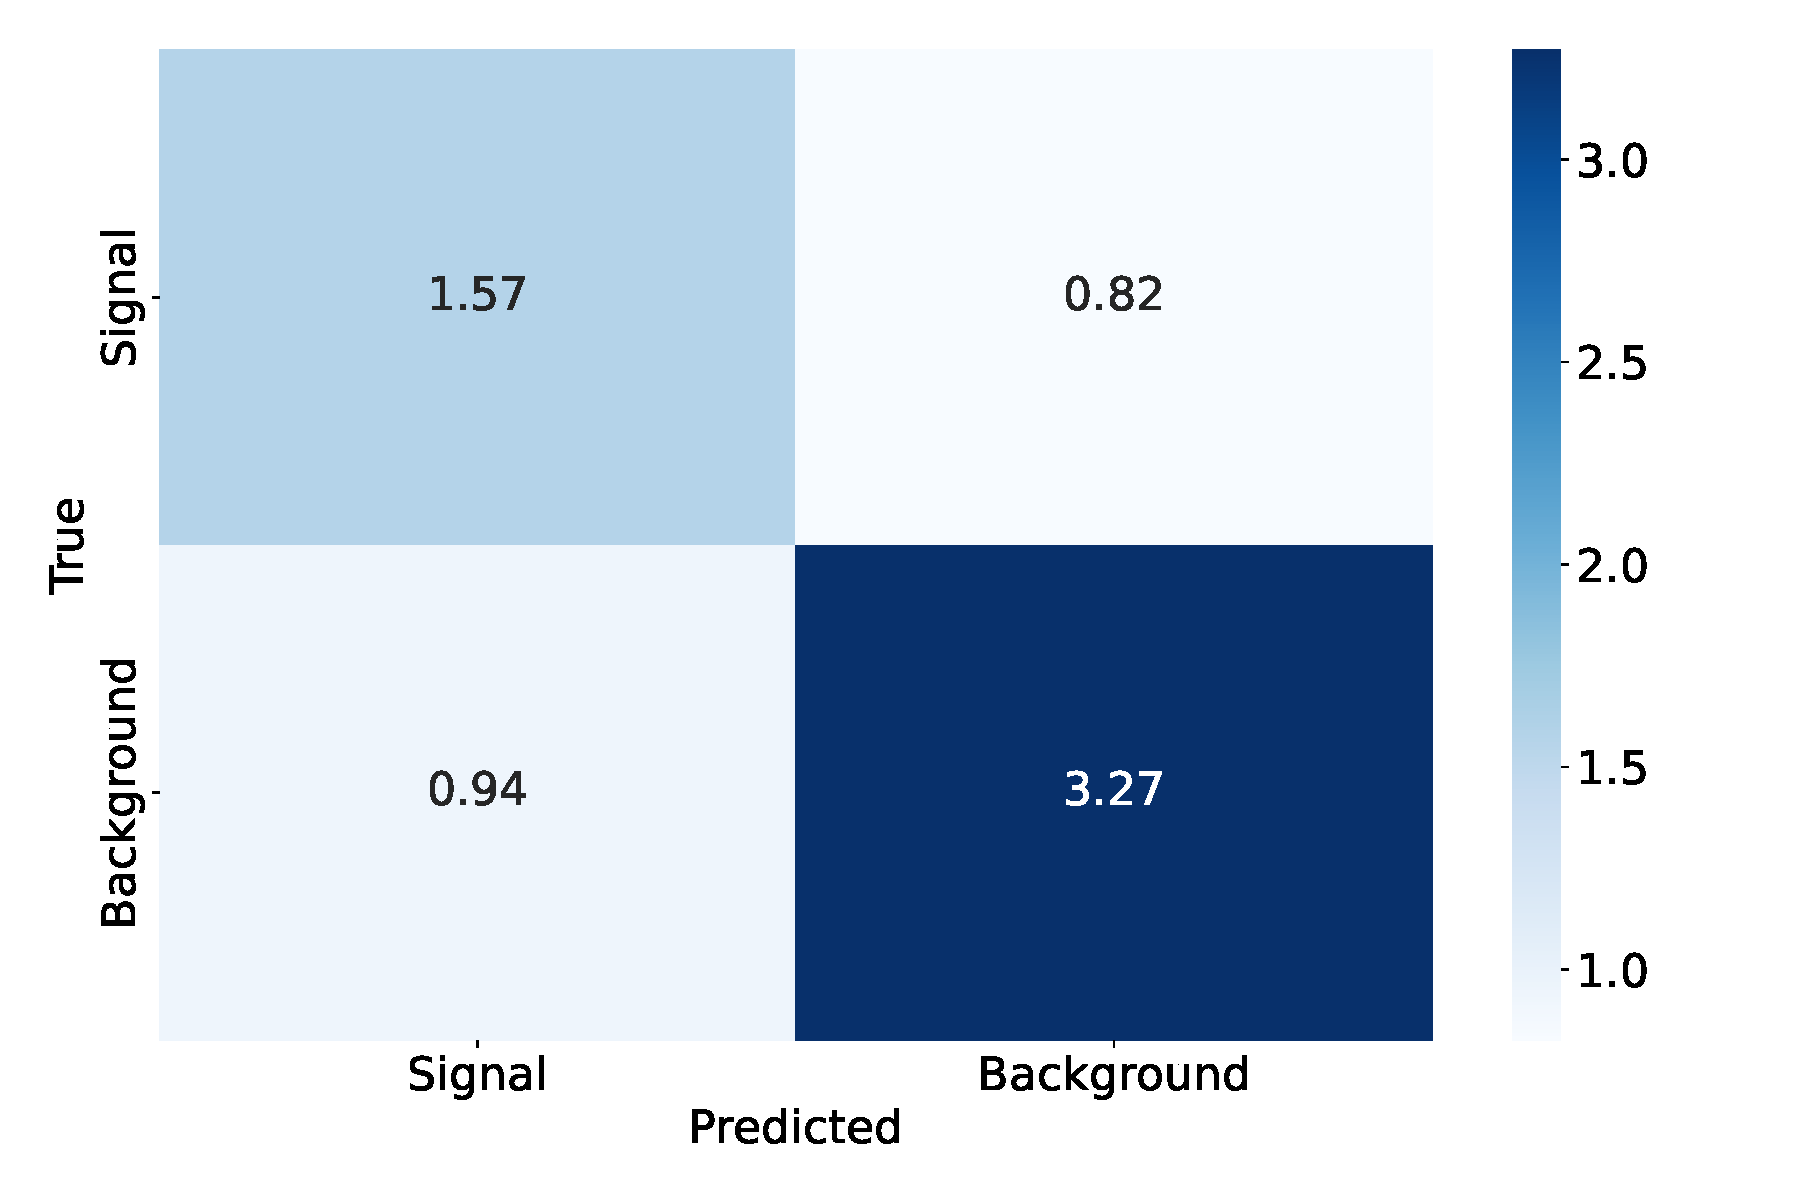
\includegraphics[trim=0.5cm 0 2cm 0, clip, width=0.8\textwidth]{figures/ml/cm/signal_argmax.pdf}
    \caption[Confusion matrix for a binary classification task]
    {Confusion matrix for a binary classification task. This confusion matrix is produced using 5-blocks
        \gls{ftt} (\autoref{sec:ftt}) trained on the extended training set (\autoref{sec:extended-set}) evaluated on the
        validation set, that contains 20\% of the \gls{sr} events. Signal refers to \tth, and background refers to all
        the other classes. The $\arg\max$ classification strategy was used.  Note that the classifier was \emph{trained}
        to differentiate between all the classes, but during evaluation, all the non-\tth events are grouped together.}
    \label{fig:cm}
\end{figure}

Binary confusion matrix naturally extends to a multi-class formulation (\autoref{fig:cm-muli}), leading to a
$|\classY| \times |\classY|$ matrix for a $|\classY|$-class classification task:

\begin{equation}
    \Cmulti_{ij} = \sum_{k=1}^{|\classY|} w_k \llbracket y_k = i \land \hat{y}_k = j \rrbracket\,,
\end{equation}

where $i$ and $j$ are the true and predicted classes, respectively. The diagonal elements of the matrix correspond to
the correctly classified events, while the off-diagonal elements correspond to the misclassified events. The
multi-class confusion matrix is not symmetric, and the sum of the elements in each row is equal to the number of events
in the corresponding true class.

\begin{figure}[htb]
    \centering
    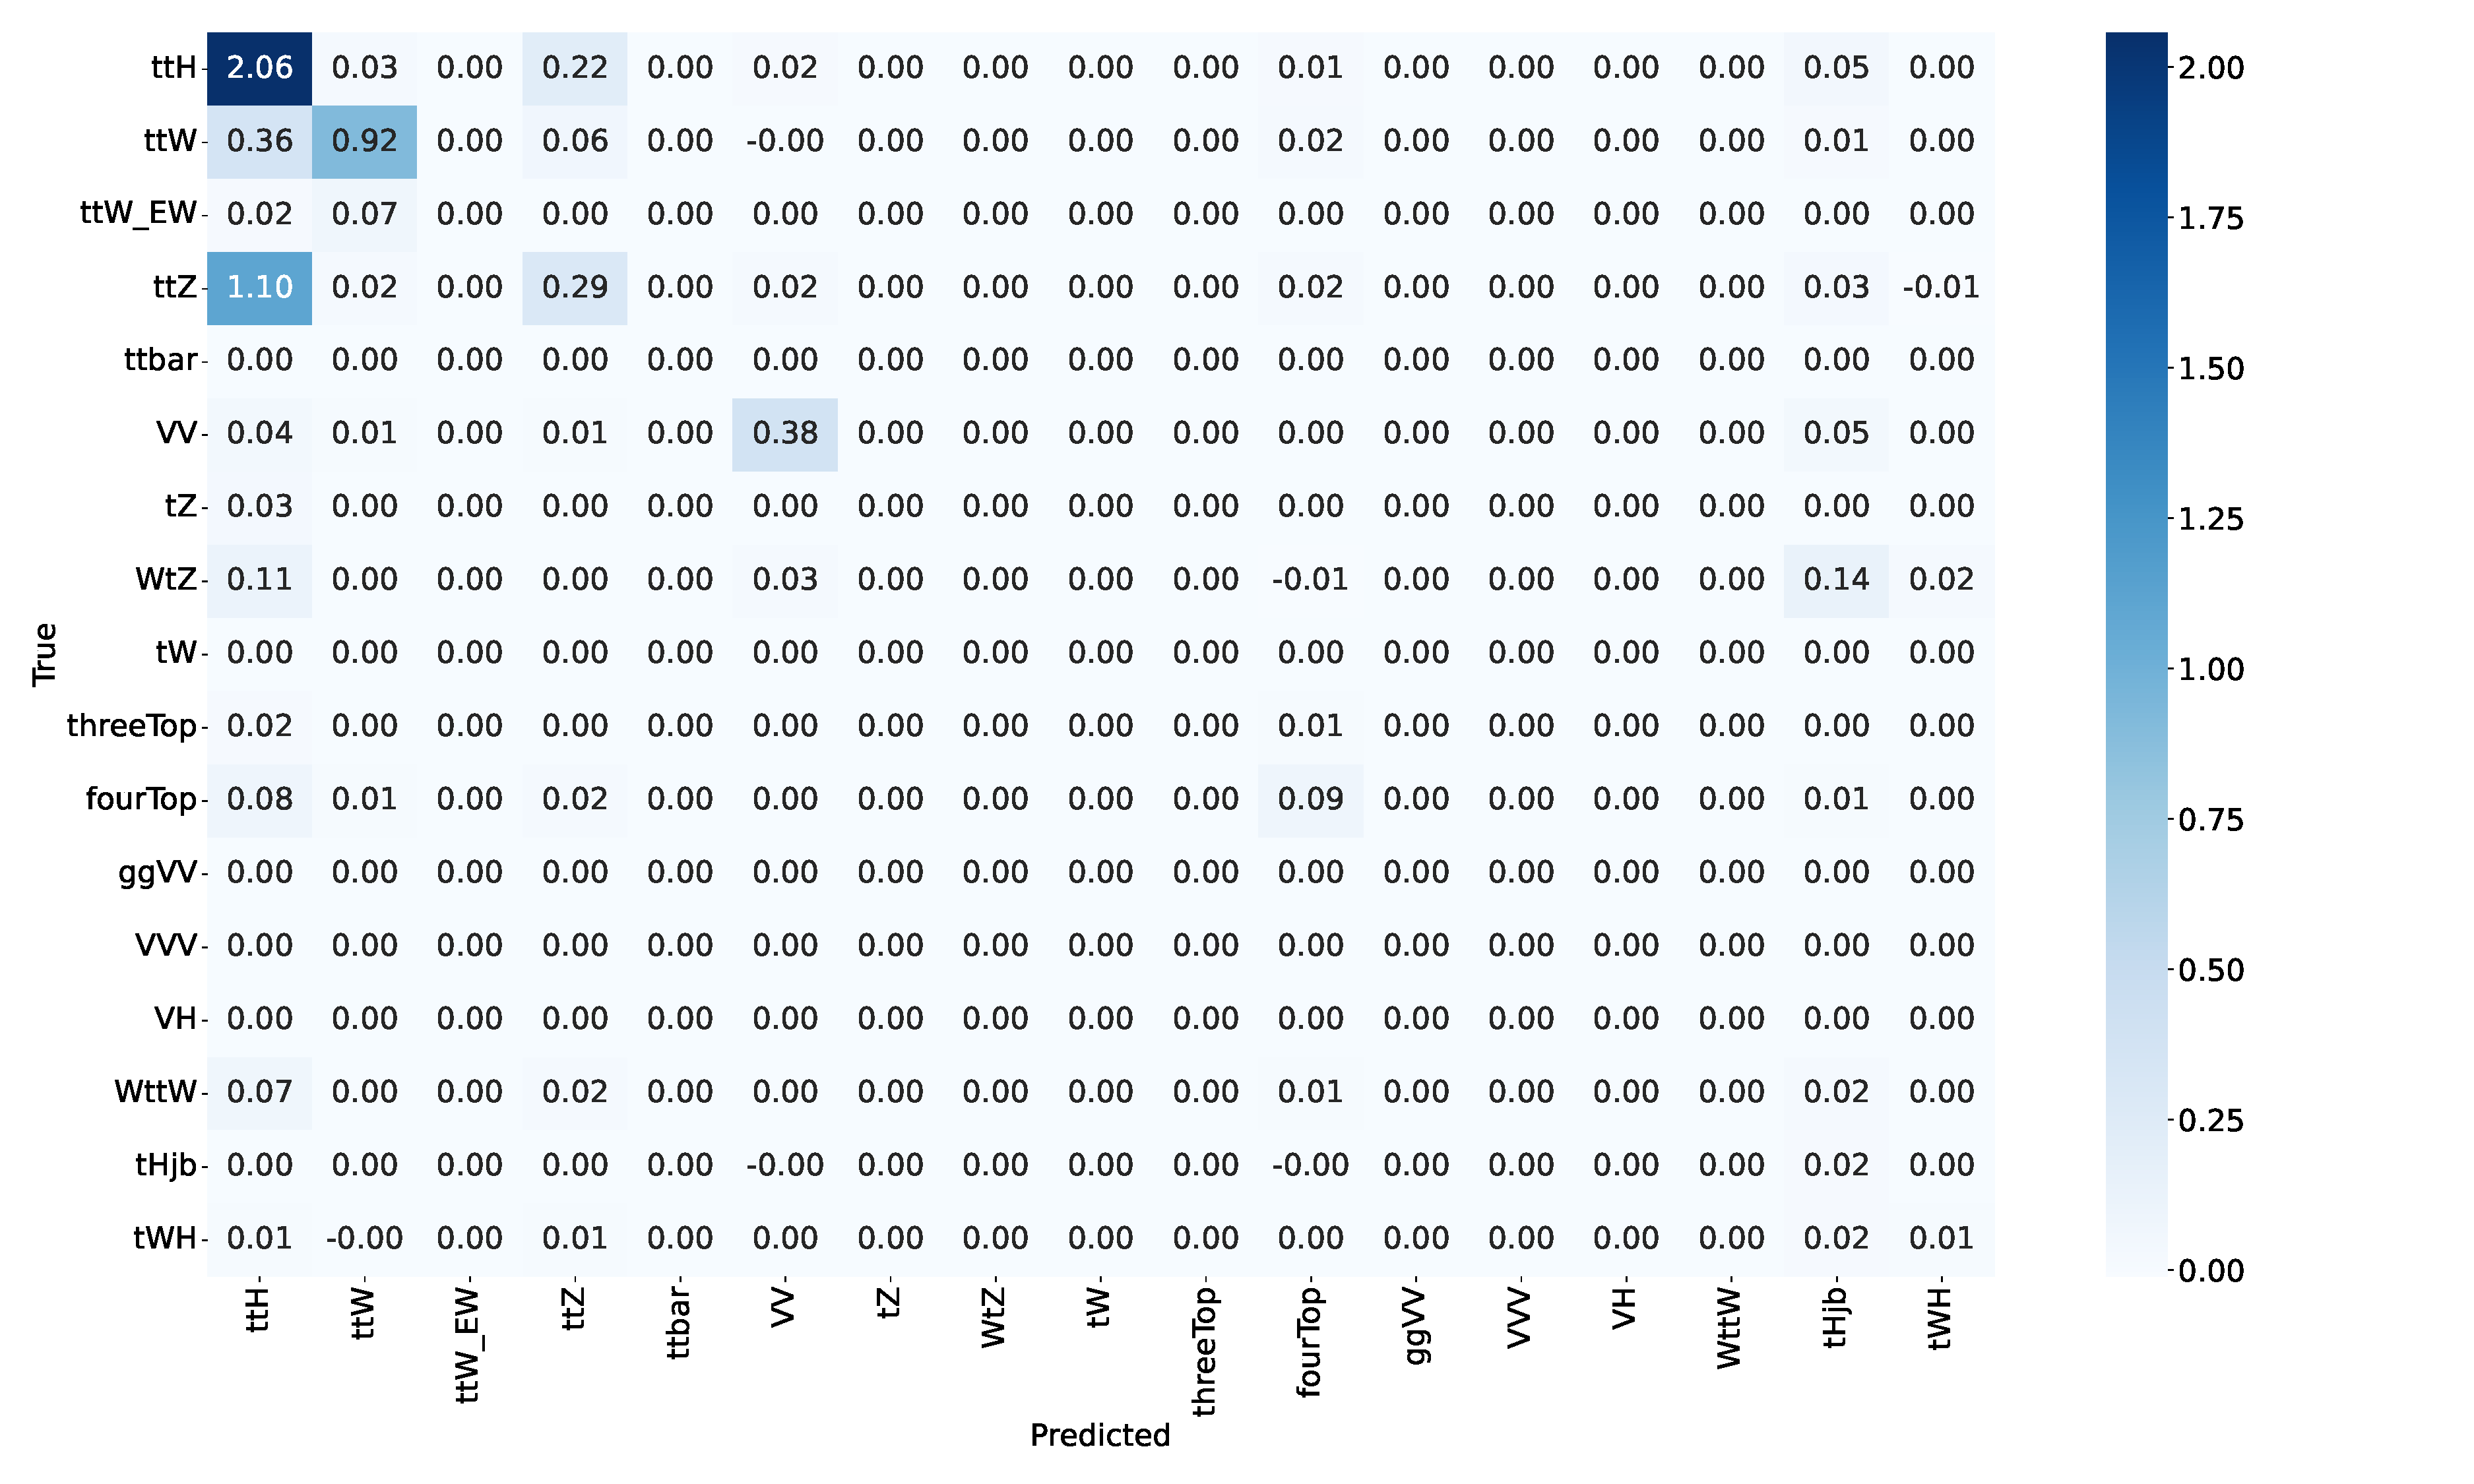
\includegraphics[trim=0.5cm 0 6cm 0, clip, width=\textwidth]{figures/ml/cm/all_argmax.pdf}
    \caption[Confusion matrix for a multi-class classification task]
    {Confusion matrix for a multi-class classification task. This confusion matrix is produced using 5-blocks
        \gls{ftt} (\autoref{sec:ftt}) trained on the extended training set (\autoref{sec:extended-set}). The
        $\arg\max$ classification strategy was used.}
    \label{fig:cm-muli}
\end{figure}

The confusion matrix serves as the basis for several other performance metrics, including accuracy, F1 score, and area
under the \gls{roc} curve (AUC-ROC).

\subsubsection{Accuracy: The Proportion of Correct Predictions}

Accuracy is the most intuitive performance metric. It is the ratio of the number of correctly classified examples
to the total number of examples (called events in particle physics). Accuracy is calculated trivially from the confusion
matrix:

\begin{align}
    \acc  = \frac{\trace \C_{ii}}{\sum_{i=1}^\classY \sum_{j=1}^\classY \C_{ij}}\,,
\end{align}

While accuracy is straightforward and commonly used, it may not always be the most representative metric, especially in
cases where the classes are imbalanced. Consider the example of our particle physics problem where we are searching for
\tth events and suppose that 90\% of the events are background and only 10\% are signal. A naïve classifier that
always predicts the background class would achieve an accuracy of 90\%. However, such a classifier would be entirely
unhelpful for the task at hand since it fails to identify any \tth events.

Certainly, the accuracy is not entirely without value, and there are contexts where it might still be useful. Even in
imbalanced scenarios, accuracy can provide a general sense of how often the classifier is correct across both the
majority and minority classes. While it may not provide a nuanced view of performance on the minority class (such as
\tth events in our case), it still provides information on the overall hit rate of correct predictions.

Additionally, in scenarios where the cost of false positives and false negatives are roughly equivalent, or when the
class distribution in the model's operational environment matches the training data, accuracy might still be a relevant
metric. It offers a quick and easily interpretable measure of performance.

However, in the specific context of searching for rare or significant events, such as \tth in particle physics, relying
solely on accuracy can be misleading. It would typically be considered alongside other metrics that give more insight
into the performance on the class of interest. Thus, while accuracy may not be the most representative metric in such
cases, it might still hold some value as part of a broader evaluation framework.

\subsubsection{Precision and Recall}

Two other important metrics which are derived from the confusion matrix are precision and recall, which are particularly
useful when dealing with imbalanced classes.

\paragraph{Precision} is the proportion of TP to all \emph{predicted} positives. Specifically, in our case, it is the
ratio of the correctly classified \tth events, to all events classified (or misclassified) as \tth. From here on, we
assume $y_1 = \tth$, and so the true \tth events correspond to the first row of the confusion matrix, while predicted
\tth events correspond to the first column. Precision is then given by

\begin{align}
    \text{Precision} = \frac{\C_{11}}{\sum_{j=1}^\classY \C_{1j}}\,.
\end{align}

\paragraph{Recall} (or sensitivity) is the proportion of TP to all \emph{actual} positives. In our case, it is the ratio
of the correctly classified \tth events to all actual \tth events (which the model might have missed by classifying them
as background). Recall is given by

\begin{align}
    \text{Recall} = \frac{\C_{11}}{\sum_{i=1}^\classY \C_{i1}}\,.
\end{align}

Precision tells us how reliable our positive predictions are,
while recall informs us how many of the actual \tth events we were able to detect. Both these metrics provide
complementary insights, and understanding the trade-off between them is essential in many real-world classification
tasks. Next, we will introduce the F1 score, a metric that combines both precision and recall to provide a balanced view
of the model's performance on both fronts.

\subsubsection{F1 Score: The Balance Between Precision and Recall}

The F1 score is the harmonic mean of precision and recall, providing a balance between the two. It is calculated as:

\begin{equation}
    \text{F1 score} = 2 \cdot \frac{\text{Precision} \cdot \text{Recall}}{\text{Precision} + \text{Recall}}
\end{equation}

\subsubsection{ROC Curve and AUC: The Trade-off Between Sensitivity and Specificity}

The \gls{roc} curve is a plot of the true positive rate (recall or sensitivity) against
the false positive rate (1 - specificity) for different classification thresholds. The area under the ROC curve
(AUC-ROC) measures the classifier's ability to distinguish between classes. A perfect classifier has an AUC-ROC of 1,
while a random classifier has an AUC-ROC of 0.5. The ROC curves for the \tth and two most dominant background processes
\ttw and \ttz are shown in \autoref{fig:rocs}.

\begin{figure}[htb]
    \centering
    \begin{subfigure}{0.32\textwidth}
        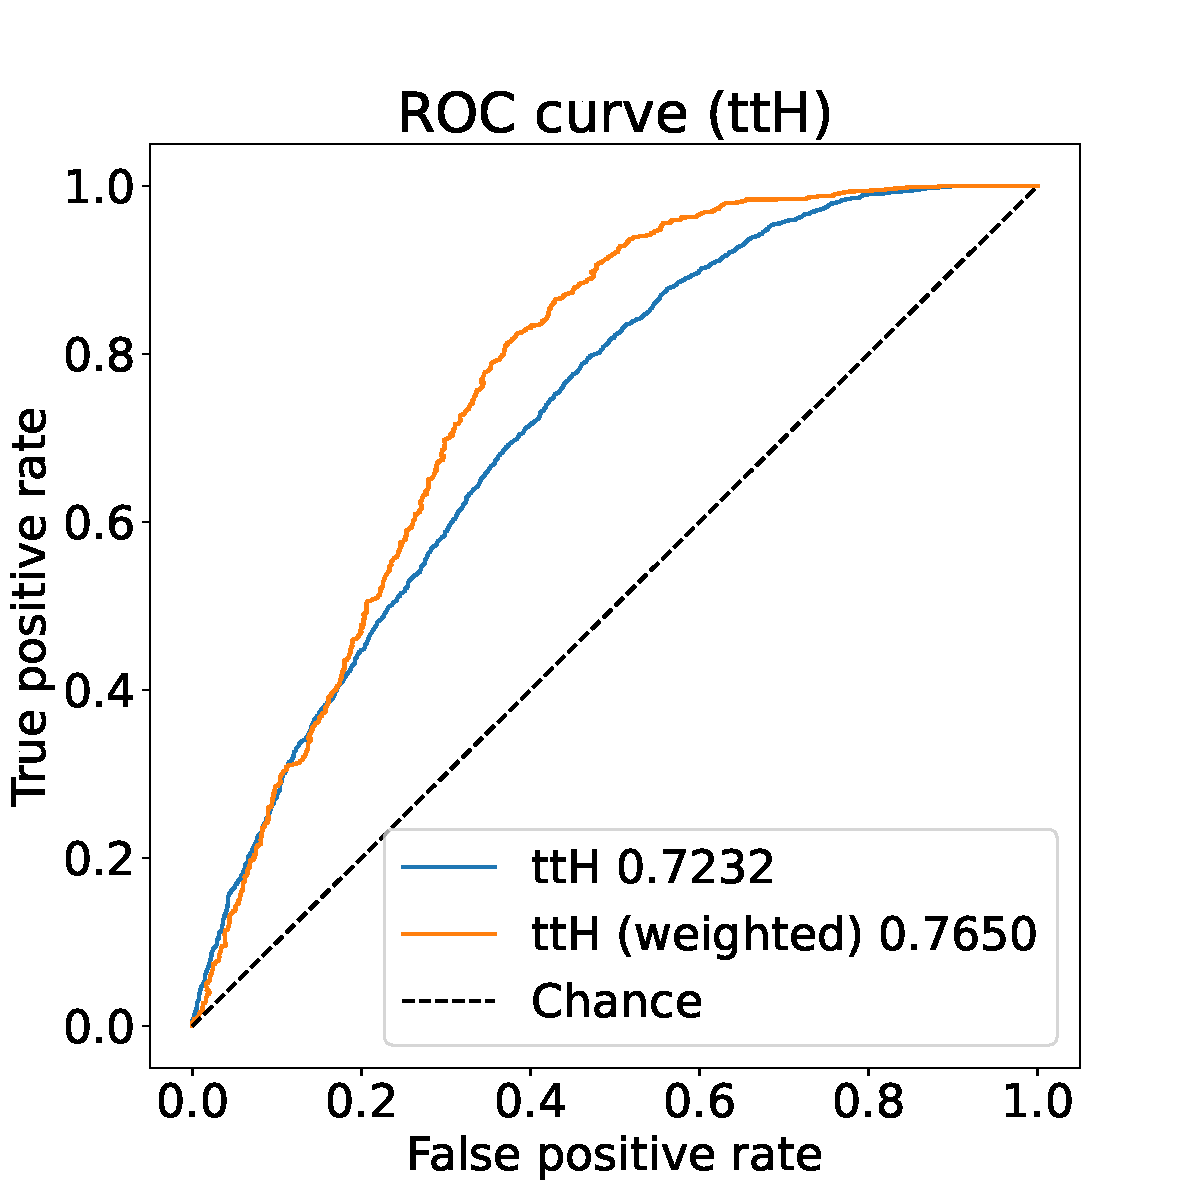
\includegraphics[width=\linewidth]{figures/ml/roc/ttH.pdf}
        \caption{\tth}
        \label{fig:roc-tth}
    \end{subfigure}
    \begin{subfigure}{0.32\textwidth}
        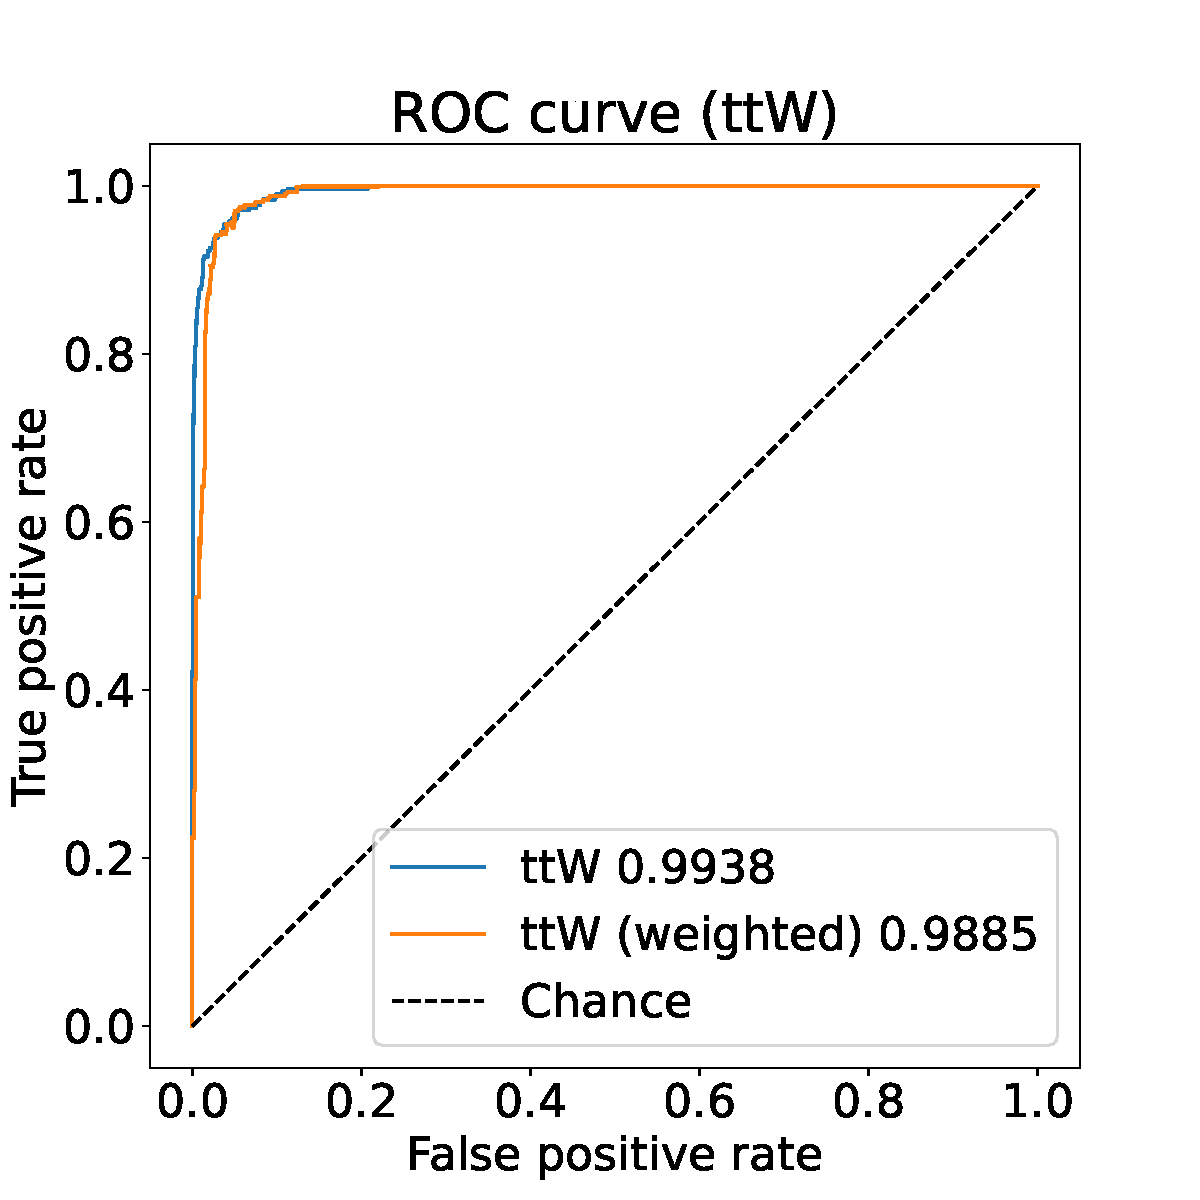
\includegraphics[width=\linewidth]{figures/ml/roc/ttW.pdf}
        \caption{\ttw}
        \label{fig:roc-ttw}
    \end{subfigure}
    \begin{subfigure}{0.32\textwidth}
        \includegraphics[width=\linewidth]{figures/ml/roc/ttZ.pdf}
        \caption{\ttz}
        \label{fig:roc-ttz}
    \end{subfigure}
    \caption[\acrshort{roc} curves for \tth, \ttz, and \ttz]
    {\gls{roc} curves for the \tth, \ttw, and \ttz computed using one process versus all other processes. The curves are produced
        using 5-blocks \gls{ftt} (\autoref{sec:ftt}) trained on the extended training set (\autoref{sec:extended-set}).
        We provide both the \glspl{roc} computed with the weighted and unweighted confusion matrices for completeness
        and comparison with the previous analysis, however, we emphasize that the weighted \glspl{roc} are the ones that
        should be used always.}
    \label{fig:rocs}
\end{figure}


These metrics, combined with the loss function, provide a comprehensive view of the classifier's performance and guide
the optimization process during training. They also provide a robust measure for comparing different classifiers or the
same classifier with different hyperparameters. Generally, one should examine all of these metrics to get a complete
picture of the classifier's performance.

% Include the architectures section
\section{V8 adaptation}

\section{\gls{sr} cut expression}
\label{appendix:cut-expression}

{\scriptsize
    \begin{verbatim}
    custTrigMatch_LooseID_FCLooseIso_DLT
    && (dilep_type && (lep_ID_0*lep_ID_1)>0)
    && ((lep_Pt_0 >= 10e3 && lep_Pt_1 >= 10e3) && (fabs(lep_Eta_0) <= 2.5 && fabs(lep_Eta_1) <= 2.5)
        && ((abs(lep_ID_0) == 13 && lep_isMedium_0 && lep_isolationLoose_VarRad_0 && passPLIVTight_0)
            || ((abs(lep_ID_0) == 11 && lep_isTightLH_0 && lep_isolationLoose_VarRad_0 && passPLIVTight_0
                && lep_ambiguityType_0 == 0 && lep_chargeIDBDTResult_recalc_rel207_tight_0 > 0.7)
                && ((!(!(lep_Mtrktrk_atConvV_CO_0 < 0.1 && lep_Mtrktrk_atConvV_CO_0 >= 0 && lep_RadiusCO_0 > 20)
                    && (lep_Mtrktrk_atPV_CO_0 < 0.1 && lep_Mtrktrk_atPV_CO_0 >= 0)))
                    && !(lep_Mtrktrk_atConvV_CO_0 <0.1 && lep_Mtrktrk_atConvV_CO_0 >= 0 && lep_RadiusCO_0 > 20))))
            && ((abs(lep_ID_1) == 13 && lep_isMedium_1 && lep_isolationLoose_VarRad_1 && passPLIVTight_1)
                || ((abs(lep_ID_1) == 11 && lep_isTightLH_1 && lep_isolationLoose_VarRad_1 && passPLIVTight_1
                    && lep_ambiguityType_1 == 0 && lep_chargeIDBDTResult_recalc_rel207_tight_1 > 0.7)
                    && ((!(!(lep_Mtrktrk_atConvV_CO_1 < 0.1 && lep_Mtrktrk_atConvV_CO_1 >= 0 && lep_RadiusCO_1 > 20)
                        && (lep_Mtrktrk_atPV_CO_1 < 0.1 && lep_Mtrktrk_atPV_CO_1 >= 0)))
                        && !(lep_Mtrktrk_atConvV_CO_1 < 0.1 && lep_Mtrktrk_atConvV_CO_1 >= 0 && lep_RadiusCO_1 > 20)))))
    && nTaus_OR==1
    && nJets_OR_DL1r_85>=1
    && nJets_OR>=4
    && ((dilep_type==2) || abs(Mll01-91.2e3)>10e3)
\end{verbatim}
}

We have kept the cuts the same as \cite{severin}, except for the cut on the \verb|nJets_OR| to \verb|>=4| to keep
consistent definition \gls{sr} definition across the group \todo{refer to the BDT group - how?}.

\section{Yields Plots}
\label{appendix:yields}

\begin{figure}[htb!]
    \centering
    \begin{subfigure}{0.45\textwidth}
        \includegraphics[width=\linewidth]{figures/yields/lep-pt-0.pdf}
        \caption{Distribution of the transverse momentum of the leading lepton.}
    \end{subfigure}\hfill%
    \begin{subfigure}{0.45\textwidth}
        \includegraphics[width=\linewidth]{figures/yields/lep-pt-1.pdf}
        \caption{Distribution of the transverse momentum of the subleading lepton.}
    \end{subfigure}
\end{figure}

\begin{figure}[htb!]
    \centering
    \begin{subfigure}{0.45\textwidth}
        \includegraphics[width=\linewidth]{figures/yields/n-jets.pdf}
        \caption{Distribution of the number of jets.}
    \end{subfigure}\hfill%
    \begin{subfigure}{0.45\textwidth}
        \includegraphics[width=\linewidth]{figures/yields/n-bjets.pdf}
        \caption{Distribution of the number of $b$-jets.}
    \end{subfigure}
\end{figure}

\begin{figure}[htb!]
    \centering
    \begin{subfigure}{0.45\textwidth}
        \includegraphics[width=\linewidth]{figures/yields/tau-width.pdf}
        \caption{Distribution of the $\tau$-jet width.}
    \end{subfigure}\hfill%
\end{figure}
\subsection{List of samples by each process}

The root directory for the files is:

{\small
\verb|/eos/atlas/atlascerngroupdisk/phys-higgs/HSG8/multilepton_ttWttH/v08/v0801/systematics-full/nominal|
}

The list of samples is given in \hyperref[tab:samples]{Table~\ref*{tab:samples}}.

\newpage

\begin{table}[h!]
    \centering
    \renewcommand{\arraystretch}{1.5}
    \caption{List of samples by each process}
    \label{tab:samples}
    \begin{tabular}{p{1.5cm}p{13.5cm}}
        \toprule
        Process      & \gls{dsid}                                                           \\
        \midrule
        $t\bar{t}H$  & p4498/346343, p4498/346344, p4498/346345                             \\
        $t\bar{t}W$  & p4416/700168, p4590/700205                                           \\
        $t\bar{t}Z$  & p4416/700168                                                         \\
        $t\bar{t}$   & p4308/410470                                                         \\
        $VV$         & \input{samples/VV.tex}                                               \\
        $ggVV$       & p4308/345705, p4396/345706, p4396/345715, p4396/345718, p4396/345723 \\
        $Zjets$      & \input{samples/Zjets.tex}                                            \\
        $Wjets$      & \input{samples/Wjets.tex}                                            \\
        $tW$         & p4308/410646, p4308/410647                                           \\
        $threeTop$   & p4308/304014                                                         \\
        $fourTop$    & p4308/410080                                                         \\
        $t\bar{t}WW$ & p4308/410081                                                         \\
        $tZ$         & p4308/410560                                                         \\
        $WtZ$        & p4308/410408                                                         \\
        $VVV$        & \input{samples/VVV.tex}                                              \\
        $VH$         & p4308/342284, p4308/342285                                           \\
        $tHjb$       & p4308/346799\_AF                                                     \\
        $tWH$        & p4308/346678\_AF                                                     \\
        \bottomrule
    \end{tabular}
\end{table}

\newpage
\subsection{Distribution of the variables inside \gls{sr}}

The following figures (\autoref{fig:distributions1} and \autoref{fig:distributions2}) show the distributions of some variables
of interest inside \gls{sr}.

\captionsetup[subfigure]{justification=centering}
\begin{figure}[htb!]
    \centering
    \begin{subfigure}{0.45\textwidth}
        \includegraphics[width=\linewidth]{figures/plots/histograms/lep_pt_0.png}
        \caption{Distribution of the transverse momentum of the leading lepton.}
        \label{fig:lep_pt_0}
    \end{subfigure}\hfill%
    \begin{subfigure}{0.45\textwidth}
        \includegraphics[width=\linewidth]{figures/plots/histograms/lep_pt_1.png}
        \caption{Distribution of the transverse momentum of the subleading lepton.}
        \label{fig:lep_pt_1}
    \end{subfigure}

    \vspace{0.5cm}

    \begin{subfigure}{0.45\textwidth}
        \includegraphics[width=\linewidth]{figures/plots/histograms/lep_Eta_0.png}
        \caption{Distribution of the pseudorapidity of the leading lepton.}
        \label{fig:lep_Eta_0}
    \end{subfigure}\hfill%
    \begin{subfigure}{0.45\textwidth}
        \includegraphics[width=\linewidth]{figures/plots/histograms/lep_Eta_1.png}
        \caption{Distribution of the pseudorapidity of the subleading lepton.}
        \label{fig:lep_Eta_1}
    \end{subfigure}
    \caption{Distributions of the variables inside \gls{sr} (part 1)}
    \label{fig:distributions1}
\end{figure}

\newpage

\begin{figure}[htb!]
    \centering
    \begin{subfigure}{0.45\textwidth}
        \includegraphics[width=\linewidth]{figures/plots/histograms/lep_Phi_0.png}
        \caption{Distribution of the azimuthal angle of the leading lepton.}
        \label{fig:lep_Phi_0}
    \end{subfigure}\hfill%
    \begin{subfigure}{0.45\textwidth}
        \includegraphics[width=\linewidth]{figures/plots/histograms/lep_Phi_1.png}
        \caption{Distribution of the azimuthal angle of the subleading lepton.}
        \label{fig:lep_Phi_1}
    \end{subfigure}

    \vspace{0.5cm}

    \begin{subfigure}{0.45\textwidth}
        \includegraphics[width=\linewidth]{figures/plots/histograms/njets.png}
        \caption{Distribution of the number of jets.}
        \label{fig:njets}
    \end{subfigure}\hfill%
    \begin{subfigure}{0.45\textwidth}
        \includegraphics[width=\linewidth]{figures/plots/histograms/nbjets.png}
        \caption{Distribution of the number of $b$-jets.}
        \label{fig:nbjets}
    \end{subfigure}
    \caption{Distributions of the variables inside \gls{sr} (part 2)}
    \label{fig:distributions2}
\end{figure}

\begin{minipage}{0.45\textwidth}
    \centering
    \begin{tabular}{c|c|c|c|c}
        $t\bar{t}H$ & \textbf{v6} & \textbf{v8} &      &       \\
        \hline
        Weighted    & 1000        & 500         & -500 & -50\% \\
        Raw         & 1000        & 500         & -500 & -50\% \\
        \hline
    \end{tabular}
    \captionof{table}{Number of ttH events in the SR for v6 and v8.}
    \label{tab:ttH_event_numbers1}
\end{minipage}\hfill%
\begin{minipage}{0.45\textwidth}
    \centering
    \begin{tabular}{c|c|c|c|c}
        \gls{sr} & \textbf{v6} & \textbf{v8} &      &       \\
        \hline
        Weighted & 1000        & 500         & -500 & -50\% \\
        Raw      & 1000        & 500         & -500 & -50\% \\
        \hline
    \end{tabular}
    \captionof{table}{Number of all the events in the SR for v6 and v8.}
    \label{tab:ttH_event_numbers2}
\end{minipage}

\clearpage \subsection{Features used}

\subsubsection{\texttt{lep\_E\_X}} The energy of the Xth lepton.

\subsubsection{\texttt{DRjj\_lead}} $\Delta R$ between the two leading jets. $\Delta R$ is a distance metric in the
$\eta-\phi$ space frequently used in particle physics.

\subsubsection{\texttt{Ptll01}} The transverse momentum of the dilepton system made up of the two leading leptons.

\subsubsection{\texttt{lep\_nTrackParticles\_X}} The number of track particles associated with the Xth lepton.

\subsubsection{\texttt{custTrigMatch\_LooseID\_FCLooseIso\_DLT}} Custom trigger matching for loosely identified and loosely
isolated leptons, likely related to the dilepton trigger

\subsubsection{\texttt{Mll01}} The invariant mass of the two leading leptons.

\subsubsection{\texttt{Mlll012}} The invariant mass of the three leading leptons.

\subsubsection{\texttt{total\_charge}} The sum of the electric charges of the particles in the event.

\subsubsection{\texttt{HT}} The scalar sum of the transverse momenta of all jets in the event.

\subsubsection{\texttt{HT\_lep}} The scalar sum of the transverse momenta of all leptons in the event.

\subsubsection{\texttt{lep\_Eta\_X}} The pseudorapidity of the Xth lepton.

\subsubsection{\texttt{nTaus\_OR\_Pt25}} The number of overlapping-removed taus with a transverse momentum above 25 GeV.

\subsubsection{\texttt{nFwdJets\_OR}} The number of overlapping-removed forward jets.

\subsubsection{\texttt{MLepMet}} The invariant mass of a lepton and the missing transverse energy vector.

\subsubsection{\texttt{taus\_DL1r\_X}} The DL1r score for the Xth tau.

\subsubsection{\texttt{lep\_isolationLoose\_VarRad\_X}} Indicates whether a lepton (where X refers to the lepton index)
passes an isolation cut with a variable radius. Looser isolation cuts allow more nearby activity in the detector.

\subsubsection{\texttt{lep\_EtaBE2\_X}} The pseudorapidity of the Xth lepton in the second layer of the electromagnetic
calorimeter.

\subsubsection{\texttt{HT\_fwdJets}} The scalar sum of the transverse momenta of all forward jets in the event.

\subsubsection{\texttt{taus\_width\_X}} The width of the Xth tau.

\subsubsection{\texttt{nJets\_OR\_DL1r\_85}} Count of jets that pass overlap removal (OR) and are b-tagged according to the
DL1r algorithm at the 85\% working point.

\subsubsection{\texttt{lep\_nInnerPix\_X}} Number of hits in the inner pixel detector associated with the lepton, where X
refers to the lepton index.

\subsubsection{\texttt{met\_phi}} The azimuthal angle of the missing transverse energy in the event.

\subsubsection{\texttt{DeltaR\_max\_lep\_bjet77}} The maximum DeltaR value between a lepton and a b-tagged jet. The "77"
may refer to the working point of the b-tagging algorithm.

\subsubsection{\texttt{MbX}} Invariant mass associated with the leading b-jet in the event

\subsubsection{\texttt{lep\_RadiusCO\_X}} Possibly the radius of the cone used for isolation of the lepton, or
alternatively a parameter associated with the trajectory of the lepton.

\subsubsection{\texttt{lep\_Mtrktrk\_atConvV\_CO\_X}} The invariant mass of track pairs at the conversion vertex for lepton
X. This might be related to photon conversions into an electron-positron pair.

\subsubsection{\texttt{lep\_Z0SinTheta\_X}} The z0 impact parameter times the sine of the lepton's polar angle.

\subsubsection{\texttt{lep\_Pt\_X}} The transverse momentum of the Xth lepton.

\subsubsection{\texttt{mjjMax\_frwdJet}} The maximum invariant mass of a pair of forward jets.

\subsubsection{\texttt{dilep\_type}} The type of dilepton event (e.g., $ee$, $\mu e$, $\mu \mu$).

\subsubsection{\texttt{eta\_frwdjet}} The pseudorapidity of the forward jet.

\subsubsection{\texttt{Mlb}} Invariant mass of a lepton and a b-jet.

\subsubsection{\texttt{taus\_RNNJetScoreSigTrans\_X}} Transformed RNN-based score for tau lepton, possibly to better
separate signal from background.

\subsubsection{\texttt{minDeltaR\_LJ\_X}} The minimum $\Delta R$ distance between the Xth lepton and any jet in the event.

\subsubsection{\texttt{nTaus\_OR}} Number of tau leptons that pass overlap removal. Overlap removal is a step in particle
reconstruction where, for instance, an object identified as both a jet and a tau would be considered only as one or the
other.

\subsubsection{\texttt{DeltaR\_min\_lep\_jet}} The minimum $\Delta R$ distance between a lepton and a jet in the event.

\subsubsection{\texttt{lep\_sigd0PV\_X}} Significance of the transverse impact parameter (d0) of the lepton X with respect
to the primary vertex (PV). This is a common variable for distinguishing prompt particles produced in the primary
collision from secondary particles produced in a decay.

\subsubsection{\texttt{taus\_eta\_X}} The pseudorapidity of the Xth tau.

\subsubsection{\texttt{HT\_jets}} The scalar sum of the transverse momenta of all jets (not forward jets) in the event.

\subsubsection{\texttt{lep\_Phi\_X}} The azimuthal angle (in radians) of the Xth lepton.

\subsubsection{\texttt{bTagSF\_weight\_DL1r\_85}} A weight applied to events based on the scale factor for b-tagging using
the DL1r algorithm at an 85\% efficiency working point. This scale factor corrects the b-tagging efficiency in Monte
Carlo simulations to match that observed in real data.

\subsubsection{\texttt{lep\_chargeIDBDTResult\_recalc\_rel207\_tight\_X}} The outcome of a BDT-based charge identification
for a lepton, recalculated with some specific settings, and applying a 'tight' threshold.

\subsubsection{\texttt{taus\_phi\_X}} The azimuthal angle (in radians) of the Xth tau.

\subsubsection{\texttt{taus\_passJVT\_X}} A boolean flag indicating whether the Xth tau passes the jet vertex tightness
(JVT) requirement.

\subsubsection{\texttt{jets\_eta}} The pseudorapidity of the jets (array).

\subsubsection{\texttt{taus\_charge\_X}} The charge of the Xth tau.

\subsubsection{\texttt{passPLIVTight\_X}} Boolean flag indicating if a lepton with high transverse momentum passes the
"tight" criteria of the Prompt Lepton Veto (PLIV), a tool for identifying non-prompt light leptons.

\subsubsection{\texttt{lep\_Mtrktrk\_atPV\_CO\_X}} The invariant mass of track pairs at the primary vertex for lepton X.
This could be related to certain types of particle decays happening at the primary collision vertex.

\subsubsection{\texttt{taus\_JetRNNSigMedium\_X}} RNN-based score for tau lepton, used to distinguish tau leptons from
jets, with 'medium' selection criteria.

\subsubsection{\texttt{minOSMll}} The minimum invariant mass of oppositely-signed dilepton pairs.

\subsubsection{\texttt{lep\_ID\_X}} The identification number for the Xth lepton.

\subsubsection{\texttt{Mllll0123}} The invariant mass of the four leading leptons.

\subsubsection{\texttt{custTrigSF\_TightElMediumMuID\_FCLooseIso\_DLT}} Custom trigger scale factor, for events with a
tight electron and a medium muon, both of which are loosely isolated, likely related to the dilepton trigger (DLT).

\subsubsection{\texttt{best\_Z\_Mll}} The invariant mass of the dilepton system that is closest to the Z boson mass.

\subsubsection{\texttt{met\_met}} The missing transverse energy in the event.

\subsubsection{\texttt{MtLep1Met}} Transverse mass between the leading lepton and missing transverse energy. Transverse
mass is often used in searches for particles that decay to a lepton and a neutrino.

\subsubsection{\texttt{lep\_ambiguityType\_X}} Type of ambiguity for lepton identification, where X refers to the lepton
index. Ambiguity could arise from several factors, such as a single track matching with multiple reconstructed
particles.

\subsubsection{\texttt{jets\_phi}} The azimuthal angle (in radians) of the jets (array).

\subsubsection{\texttt{lep\_isMedium\_X}} Boolean flag indicating if a lepton passes the 'medium' selection criteria.

\subsubsection{\texttt{taus\_RNNJetScore\_X}} RNN-based score for tau lepton, used to distinguish tau leptons from jets.

\subsubsection{\texttt{MtLepMet}} The transverse mass of a lepton and the missing transverse energy vector.

\subsubsection{\texttt{DeltaR\_min\_lep\_jet\_fwd}} The minimum $\Delta R$ distance between a lepton and a forward jet in the event.

\subsubsection{\texttt{jets\_e}} The energy of the jets (array).

\subsubsection{\texttt{minOSSFMll}} The minimum invariant mass of oppositely-signed, same-flavor dilepton pairs.

\subsubsection{\texttt{nJets\_OR}} The number of overlapping-removed jets.

\subsubsection{\texttt{total\_leptons}} The total number of leptons in the event.

\subsubsection{\texttt{taus\_numTrack\_X}} The number of tracks associated with the Xth tau.

\subsubsection{\texttt{HT\_taus}} Scalar sum of the transverse momenta ($P_t$) of all tau leptons in the event.

\subsubsection{\texttt{taus\_passEleOLR\_X}} A boolean flag indicating whether the Xth tau passes the electron overlap
removal.

\subsubsection{\texttt{HT\_inclFwdJets}} The scalar sum of the transverse momenta of all jets, including forward jets, in
the event.

\subsubsection{\texttt{DRll01}} The $\Delta R$ distance between the two leading leptons.

\subsubsection{\texttt{taus\_JetRNNSigLoose\_X}} RNN-based score for tau lepton, used to distinguish tau leptons from
jets, with 'loose' selection criteria.

\subsubsection{\texttt{taus\_pt\_X}} The transverse momentum of the Xth tau.

\subsubsection{\texttt{bTagSF\_weight\_DL1r\_77}} A weight applied to events based on the scale factor for b-tagging using
the DL1r algorithm at an 77\% efficiency working point. This scale factor corrects the b-tagging efficiency in Monte
Carlo simulations to match that observed in real data.

\subsubsection{\texttt{flag\_JetCleaning\_LooseBad}} A flag variable indicating whether a jet passes a loose cleaning cut
to remove bad or noisy jets from the analysis.

\subsubsection{\texttt{taus\_fromPV\_X}} A boolean flag indicating whether the Xth tau comes from the primary vertex.

\subsubsection{\texttt{best\_Z\_other\_MtLepMet}} The transverse mass between the lepton and missing transverse energy for
the event that best reconstructs a Z boson using other criteria.

\subsubsection{\texttt{nJets\_OR\_DL1r\_77}} Count of jets that pass overlap removal (OR) and are b-tagged according to the
DL1r algorithm at the 77\% working point.

\subsubsection{\texttt{jets\_pt}} The transverse momentum of the jets (array).

\subsubsection{\texttt{lep\_isTightLH\_X}} Boolean flag indicating if a lepton passes the 'tight' Likelihood-based
identification criteria.

\subsubsection{\texttt{taus\_JetRNNSigTight\_X}} RNN-based score for tau lepton, used to distinguish tau leptons from
jets, with 'tight' selection criteria.

\subsubsection{\texttt{sumPsbtag}} The sum of b-tagging weights for jets in the event.

\subsubsection{\texttt{taus\_decayMode\_X}} The decay mode of the Xth tau.

\subsubsection{\texttt{dEta\_maxMjj\_frwdjet}} The maximum difference in pseudorapidity ($\eta$) between two forward jets.

\subsubsection{\texttt{max\_eta}} The maximum pseudorapidity among all particles in the event.

\subsubsection{\texttt{best\_Z\_other\_Mll}} The invariant mass of the dilepton system that is closest to the Z boson mass,
not considering the leading leptons.

\subsubsection{\texttt{taus\_passEleBDT\_X}} Flag indicating if a tau lepton passes the Electron Boosted Decision Tree
discriminator.

\begin{figure}[hbtp]
    \centering
    \includegraphics[width=\textwidth]{figures/ml/features/top20.pdf}
    \caption{Feature importance for the top 20 most important features. Feature importance was calculated using the
        \gls{ig} method \cite{ig}.}
    \label{fig:feature_importance}
\end{figure}

\clearpage

% Generate the results figure
\begin{figure}
    \centering
    \includegraphics{example-image-a}
    \caption{Results of all the notable techniques \todo{todo}}
    \label{tab:results}
\end{figure}

% This chapter describes the methodology used in this study. It includes the formulation of the problem, the evaluation metrics used, and the architectures tested.
\chapter{Methodology}
\label{ch:Methodology}

% Include the formulation section
\section{Problem Formulation}
\label{sec:formulation}

\todo{proofread}

\glsreset{erm}
\subsection[Empirical Risk Minimization]{\gls{erm}}

As stated before, our primary objective in this thesis is to distinguish the \tth events from other events of the other
detected by the \gls{atlas} detector. Given an observation $\bm{x} \in \mathcal{X}$, we want to predict its
corresponding class label $y \in \mathcal{Y}$. Here $\mathcal{X}$ denotes the space of all possible observations (in
our case this corresponds to the different measurements of the event), and $\mathcal{Y}$ denotes the space of all
the class labels we are differentiating between. We can further split the problem into either a binary classification
(seeking to differentiate between \tth (signal) and not \tth (background)) or a multi-class classification (seeking to
correctly discriminate between each of the processes - \tth, \ttw, \ttz, \ttbar, etc.).

As we approach this task as a supervised learning problem (recall \autoref{sec:mc}), we assume that a set of labeled
observations $\ttrn = {(\bm{x}_i, y_i)}_{i=1}^N$ is provided.  Here $\bm{x}_i \in \mathbf{X}$ is a feature vector
representing different properties (features) of an event and $y_i \in \mathbf{Y}$ is its corresponding true class label.
We assume there exists a joint probability distribution $P(\bm{x}, y)$ over the observations $\bm{x}$ and their
corresponding class labels $y$. Then, we require the examples in the training set $(\bm{x}_i, y_i) \in \ttrn$ to be
drawn \gls{iid} from the joint distribution $P(\bm{x}, y)$.


We also assume that there is a non-negative real-valued loss function $L(y, \hat{y})$ that quantifies the
discrepancy between the true label $y$ and the predicted label $\hat{y}$. The common example of such a loss function
would be a zero-one loss function, which is defined as

\begin{equation}
    L_{0/1}(y, \hat{y}) = \begin{cases}
        0 & \text{if } y = \hat{y} \\
        1 & \text{otherwise}
    \end{cases}\,.
\end{equation}

The goal is to find the best hypothesis $h^* \in \mathcal{H}:
    \mathbf{X} \rightarrow \mathbf{Y}$ that would minimize the expected loss over the joint distribution $P(\bm{x}, y)$:

\begin{equation}
    h^* = \argmin_{h \in \mathcal{H}} \mathbb{E}_{(\bm{x}, y) \sim P(\bm{x}, y)}[L(y, h(\bm{x}))]\,.
\end{equation}

In practice, we do not have access to the joint distribution $P(\bm{x}, y)$, but only to the training set $\ttrn$. To
tackle this problem, we use the \gls{erm} principle \cite{risk-minimization}, which states that the best hypothesis
$h^*$ is the one that minimizes the empirical risk over the training set $\ttrn$:

\begin{equation}
    \hat{h} = \argmin_{h \in \mathcal{H}} R_\ttrn(h) = \argmin_{h \in \mathcal{H}} \frac{1}{N} \sum_{i=1}^{N} L(y_i, h(\bm{x}_i))\,.
\end{equation}










\subsection{Validation and Test Sets}

Consider, for example the following "cheating" classifier:

\begin{equation}
    h(\bm{x}) = \begin{cases}
        y_i & \text{if } \exists i : \bm{x} = \bm{x}_i \\
        y_0 & \text{otherwise}
    \end{cases}\,.
\end{equation}


This classifier would have zero empirical risk, but would perform poorly on unseen data (would not generalize well).
This is referred to as overfitting (see \autoref{fig:standard-losses}). Generally, in case of an unconstrained
hypothesis space $\mathcal{H}$, we have no guarantee that the empirical risk $R_\ttrn(h)$ is a good approximation of the
true risk $R(h)$.


Specifically, the problem in this case is that the prediction $\hat{y}_i$ depends not only on the observation
$\bm{x}_i$, but also on the labels $y_1, \dots, y_N$. Consider, for example, a \gls{nn} classifier $h_\nnparams$ with trainable
parameters $\nnparams$. When training $h_\nnparams$ on the training set by back-propagation, $\nnparams$  becomes implicitly
conditioned on the true labels $y^1, \dots, y^s$ that the network has encountered before ($s$ denotes the training step).
This violates the \gls{iid} assumption and thus the empirical risk $R_\ttrn(h_\nnparams)$ is not a good approximation of
the true risk $R(h_\nnparams)$ anymore.


To address this issue and more accurately assess the generalization ability of the classifier $h$, We would need a
separate set $\tval \sim P(\bm{x}, y)$ that would provide an unbiased estimate of the true risk $R(h)$. This set is
called the validation set. Validation set is used to compare the performance of different
classifiers. Consider two classifiers $h_1$ and $h_2$, where the risk on the training set is $R_\ttrn(h_1) <
    R_\ttrn(h_2)$, but the risk on the validation set is $R_\tval(h_1) > R_\tval(h_2)$. In this case, we would prefer the
classifier $h_2$ over $h_1$ as it generalizes better to unseen data. The specific case is often seen with the \gls{nn}
classifiers, where the classifier $h$ is parametrized by $\nnparams$. Then essentially we compare $h_1 = h_{\nnparams_1}$ and
$h_2 = h_{\nnparams_2}$, where $\nnparams_1$ and $\nnparams_2$ are two different sets of parameters. The process of selecting
the best classifier $h^*$ from a set of classifiers $\mathcal{H}$ is called model selection.

\begin{figure}[htb]
    \centering
    \begin{minipage}[t][\height][t]{0.47\textwidth}
        \includegraphics[width=\textwidth]{figures/ml/training/standard-ts-losses.png}
        \caption{\acrshort{ftt} with 2 blocks and 256 embedding size training on the standard training set.}
        \label{fig:standard-losses}
    \end{minipage}
    \hfill
    \begin{minipage}[t][\height][t]{0.47\textwidth}
        \includegraphics[width=\textwidth]{figures/ml/training/extended-ts-losses.png}
        \caption{\acrshort{ftt} with 5 blocks, 256 embedding size, and 20\% dropout training on the \emph{extended} training
            set.} \label{fig:extended-losses}
    \end{minipage}
    \caption[Training and validation losses during the training process with and without extended training set.]
    {Training and validation losses during the training process with and without extended training set.
        \autoref{fig:standard-losses} shows the training of the \acrshort{ftt} with 2 blocks (see \autoref{sec:ftt}) on the
        standard training set. Because of the lack of training samples, and high capacity of the model, we observe
        overfitting. The training loss continues to decrease while the validation loss starts to increase. The
        checkpoint with the validation loss is the lowest is then used as the final model. This is referred to as early
        stopping. The best way to prevent overfitting is to get more training data (see
        \autoref{sec:extended-set}). If that is not possible, one might also consider augmentation techniques, or
        regularization - dropout (see \autoref{sec:dropout}), weight decay etc. \autoref{fig:extended-losses} shows the
        training of the \acrshort{ftt} with 5 blocks (see \autoref{sec:ftt}) on the extended training set. Also, the 20\%
        dropout is introduced. We observe now only a slight overfitting, which means that the model has generalized
        a lot better.}
    \label{fig:losses}
\end{figure}

The caveat of using the validation for model selection is that in doing so we are implicitly fitting to the validation set,
as now our best classifier $h^*$ is also conditioned on the evaluations of the other classifiers on the validation set.
To address the similar issue, a third set is normally introduced, called the test set $\ttst \sim P(\bm{x}, y)$. The test
set should be used only once to assess the performance of the fully-trained classifier $h^*$.




\todo{But then why we don't use the test set in our thesis???}





\subsection{Training}

The process of finding the best hypothesis $h^*$ is called training (or learning). In the context of \gls{erm}, this
further reduces to minimization of the empirical risk $R_\ttrn(h)$. As described before, the empirical risk is an
expectation of the loss function $L(y, h(\bm{x}))$ over the training set $\ttrn$. Thus, the choice of the loss function
will determine the available training algorithms.

This work focuses on training the \gls{nn} classifiers. \gls{nn} can be formally described as a parametric model
parametrized by a vector of parameters $\nnparams$. \glspl{nn} are generally composed of multiple layers
$f_{\nnparams_i}^1, \dots f_{\nnparams_L}^D$ ($D$ denotes the total number of layers - depth of the network), where
each layer $f_{\nnparams_i}^i$ is a parametric function parametrized by $\nnparams_i$.  \glspl{nn} can take different
architectures, a common one\footnote{In this thesis we use an adaptation of \glspl{resnet} to tabular data and
    \glspl{ftt}, which are both a special cases of feed-forward \glspl{nn}.} is a feed-forward \gls{nn} where the output
of the layer $f_{\nnparams_i}^i$ is fed as an input to the next layer $f_{\nnparams_{i+1}}^{i+1}$. The output
of the last layer $f_{\nnparams_L}^D$ is the output of the network $h_\nnparams$. Alternative to feed-forward
\glspl{nn} would be the network that contain cycles (e.g.  \glspl{rnn}\footnote{Overview of the different types of
    \glspl{rnn} \url{https://paperswithcode.com/methods/category/recurrent-neural-networks}.} \cite{rnn,lstm}).

The parameter vector of the whole neural network can be seen as a concatenation of the parameters of the individual
layers:

\begin{equation}
    \nnparams = \begin{bmatrix}
        \nnparams_1 \\
        \vdots      \\
        \nnparams_L
    \end{bmatrix}\,.
\end{equation}

The goal is then to find the optimal set of parameters $\nnparams^*$ that minimizes the empirical risk $R_\ttrn(h_\nnparams)$.

Training \glspl{nn} efficiently involves the use of gradient-based optimization algorithms where the gradient of the
empirical risk $R_\ttrn(h_\nnparams)$ with respect to the parameters $\nnparams$ is computed and used to update the parameters
$\nnparams$ in the direction of the steepest descent. The gradient of the empirical risk $R_\ttrn(h_\nnparams)$ with respect to
the parameters $\nnparams$ can be computed using the chain rule:

\begin{equation}
    \nabla_\nnparams R_\ttrn(h_\nnparams) = \nabla_\nnparams \frac{1}{N} \sum_{i=1}^{N} L(y_i, h_\nnparams(\bm{x}_i)) = \frac{1}{N} \sum_{i=1}^{N} \nabla_\nnparams L(y_i, h_\nnparams(\bm{x}_i))\,,
\end{equation}

and is essentially an average of the gradients of the loss function $L(y_i, h_\nnparams(\bm{x}_i))$ with respect to the
parameters $\nnparams$ over the training set $\ttrn$. During the update step, the parameters $\nnparams$ are updated in the
direction of the steepest descent:

\begin{equation}
    \nnparams \leftarrow \nnparams - \alpha \nabla_\nnparams R_\ttrn(h_\nnparams)\,,
\end{equation}

where $\alpha$ is the learning rate, a hyperparameter controlling the size of the update step. In practice,
instead of computing the gradient over the whole training set $\ttrn$, the gradient is computed on the so-called
mini-batches of the training data. This gradient, computed on the mini-batch acts as an unbiased estimate of the true
gradient. This approach is called \gls{sgd} and is the most common optimization algorithm used for training
\glspl{nn}\footnote{Aside from having low computational and
    memory requirements, being able to learn online, \gls{sgd} has some other advantages, such as being able to escape
    local minima, generalize better and provide the regularization effect - all consequences of an inherent noise in the
    gradient estimate.}.
Throughout our experiments we use an improvement of \gls{sgd} called \gls{adamw} \cite{adam, adamw} which is an adaptive
learning rate optimization algorithm that uses the first and second moments of the gradient to adapt the learning rate
dynamically.

Computation of the gradient of the loss function $L(y_i, h_\nnparams(\vec{x}_i))$ with respect to the parameters \nnparams
is done using the chain rule. The chain rule is a formula for computing the derivative of the composition of two or more
functions:

\begin{equation}
    \dv{(\vec{f} \circ \vec{g})}{\vec{x}} = \dv{\vec{f}}{\vec{g}} \dv{\vec{g}}{\vec{x}}\,,
\end{equation}

where $\vec{f}$ and $\vec{g}$ are functions of $\vec{x}$.

In the context of \glspl{nn}, the chain rule is used to compute the gradient of the loss function with respect to the
parameters \nnparams by an iterative approach. First, let the outputs of the individual layers are recorded during the
forward pass (or forward propagation):

\begin{align}
    \vec{z}^i & = \vec{f}^i(\vec{z}^{i-1}) \quad i = 1, \dots, L \\
    \vec{z}^0 & = \vec{x}\,,
\end{align}

where $\vec{z}^i$ is the output of the $i$-th layer and $\vec{z}^0 = \vec{x}$ is the input to the first layer. Then, we
can compute the gradients with respect to the outputs of the layers:

\begin{align}
    \vec{\delta}^D     & = \dv{L}{\vec{f}^D}                                                                              \\
    \vec{\delta}^{D-1} & = \dv{L}{\vec{f}^D} \dv{\vec{f}^D}{\vec{z}^{D-1}} = \vec{\delta}^D \dv{\vec{f}^D}{\vec{f}^{D-1}} \\
    \vec{\delta}^{D-2} & = \vec{\delta}^{D-1} \dv{\vec{f}^{D-1}}{\vec{f}^{D-2}}                                           \\
                       & \vdots \nonumber                                                                                 \\
    \vec{\delta}^1     & = \vec{\delta}^2 \dv{\vec{f}^2}{\vec{f}^1}\,.
\end{align}

Then, the
gradient of the loss function with respect to the parameters of each layer $\nnparams_i$ is computed as

\begin{align}
    \dv{L}{\nnparams_D}     & = \dv{L}{\vec{f}^D} \dv{\vec{f}^D}{\nnparams_{D}} = \vec{\delta}^D \dv{\vec{f}^D}{\nnparams_{D}} \\
    \dv{L}{\nnparams_{L-1}} & = \dv{L}{\vec{f}^D} \dv{\vec{f}^D}{\vec{f}^{D-1}} \dv{\vec{f}^{D-1}}{\nnparams_{L-1}} =\
    \vec{\delta}^{D-1} \dv{\vec{f}^{D-1}}{\nnparams_{D-1}}                                                                     \\
    \dv{L}{\nnparams_{D-2}} & = \vec{\delta}^{D-2} \dv{\vec{f}^{D-2}}{\nnparams_{D-2}}                                         \\
                            & \vdots \nonumber                                                                                 \\
    \dv{L}{\nnparams_{1}}   & = \vec{\delta}^1 \dv{\vec{f}^1}{\nnparams_{1}}\,.
\end{align}

The chain rule is the reason why \glspl{nn} are so successful in practice. It allows for the efficient computation of
the gradient even for very deep \glspl{nn}.






\subsection{Cross-entropy loss}

In order for the back-propagation to work, all the functions must be differentiable. The zero-one loss function that we
have used in the previous section does not conform to this requirement. In practice, when training \glspl{nn} on the
classification tasks, the cross-entropy loss function is used. Cross-entropy loss operates on the probabilities, rather
than on the predicted label, thus making it differentiable and suitable to be used in the back-propagation algorithm.
The cross-entropy loss function is defined as:

\begin{equation}
    L(y_i, \vec{h}(\vec{x}_i)) = -\sum_{j = 1}^{|\textbf{Y}|} \llbracket y_i = y_j \rrbracket \log(h_j(\vec{x}))\,.
\end{equation}

In certain scenarios, such as imbalanced datasets, it may be beneficial to apply different weights to different classes.
Class weights are used to give more importance to under-represented classes, effectively balancing the contribution of
each class to the overall loss. This helps the learning algorithm focus more on the minority class, which may be of
particular interest or significance.

For example, consider a medical diagnosis application where 95\% of the samples are negative ($y = 0$) and only 5\% are
positive ($y = 1$) for a specific condition. Training a model on this dataset without any adjustments may lead to a
classifier that almost always predicts the negative class, since it's encountering it much more often. Such a skewed
prediction can be problematic in critical applications, as missing the rare positive cases could have serious
consequences. To alleviate this issue, class weights can be introduced to the loss function to give equal importance to
both classes. The modified loss function is:

\begin{equation}
    L(y_i, \vec{h}(\vec{x}_i)) = -\sum_{j = 1}^{|\textbf{Y}|} \llbracket y_i = y_j \rrbracket w_j \log(h_j(\vec{x}))\,.
\end{equation}

Here weights $w_1, \dots, w_{|\textbf{Y}|}$ are assigned to each class, where $w_i$ is calculated as:

\begin{equation}
    w_i = \frac{|\{y \sim \textbf{Y} \mid y = i\}|}{|\textbf{Y}| \sum_{i = 1}^{|\textbf{Y}|} w_i} \quad i = 1, \dots, |\textbf{Y}|\,.
\end{equation}

Essentially, we count the number of examples of class $i$ and divide it by the total number of examples in the dataset.
Then we normalize\footnote{This is optional, but helpful - inverse frequencies can have a large range, especially if
    there is extreme imbalance between the classes. Keeping the weights in the [0, 1] range also help interpretability.}
the weights so that they sum up to 1.


Similarly, the way the cross-entropy is defined, we can also introduce a more refined sample-wise weighting. In this
case, the loss function would is defined as:

\begin{equation}
    L(y_i, \vec{h}(\vec{x}_i)) = -\sum_{j = 1}^{|\textbf{Y}|} \llbracket y_i = y_j \rrbracket w_i \log(h_j(\vec{x}))\,.
\end{equation}

Here we should note that $w_i$ is not the same as the class weight $w_i$ from the previous example. In this case, $w_i$
is a weight assigned to each sample, rather than to each class, which we note by using the same index $i$ as in the
$y_i$ and $\vec{x}_i$. This formulation is not commonly used, bt was explored by the previous analysis
\cite{severin,jan}, thus we include it here for completeness. More details are given in \autoref{sec:weights}.



% Include the evaluation section
\section{Evaluating the Classifier Performance}
\label{sec:evaluation}

During evaluation, it is essential to go beyond the loss function and consider different metrics that shed
light on various aspects of the model's performance. These metrics offer a more comprehensive understanding of how well
the classifier is doing. For example, in a binary classification problem such as diagnosing a specific medical
condition, merely looking at the loss might not reveal how well the model is identifying positive cases among the
minority class.

Classification metrics include measures like Accuracy, which gives an overall picture of correct classifications, and
Precision and Recall, which focus on the model's performance with respect to a specific class. Other metrics like the
F1-Score provide a balance between Precision and Recall, and AUC-ROC measures the ability of the model to discriminate
between positive and negative classes. Choosing the right combination of these metrics is vital, as it guides the
optimization during training and influences the model's generalization to unseen data.

Understanding and selecting the appropriate classification metrics ensures alignment with the problem's unique
requirements and goals, enhancing the model's utility and effectiveness in real-world applications.


\subsubsection{Confusion Matrix}
\label{sec:weihted-cm}

The confusion matrix provides a comprehensive view of the classifier's performance. For a binary classification task, it
is a $2\times2$ matrix where the rows correspond to the true classes and the columns correspond to the predicted classes:

\begin{equation}
    \Cbin = \begin{pmatrix}
        \text{TP} & \text{FP} \\
        \text{FN} & \text{TN} \\
    \end{pmatrix}
\end{equation}

\begin{align}
    \text{TP} & = \sum_{i=1}^{N} \llbracket y_i = 1 \land \hat{y}_i = 1 \rrbracket    \\
    \text{FP} & = \sum_{i=1}^{N} \llbracket y_i = 0 \land \hat{y}_i = 1 \rrbracket    \\
    \text{FN} & = \sum_{i=1}^{N} \llbracket y_i = 1 \land \hat{y}_i = 0 \rrbracket    \\
    \text{TN} & = \sum_{i=1}^{N} \llbracket y_i = 0 \land \hat{y}_i = 0 \rrbracket\,,
\end{align}

where TP (true positive) is the number of positive instances correctly identified as positive, TN (true negative) is the
number of negative instances correctly identified as negative, FP (false positive) is the number of negative instances
incorrectly identified as positive (Type I error), and FN (false negative) is the number of positive instances
incorrectly identified as negative (Type II error).

As explained in \autoref{sec:mc}, the event weights should always be used when evaluating the classifier's
performance. Otherwise, the results we obtain are not representative of the real-world performance. All metrics
we use thus stem from the \emph{weighted} confusion matrix, defined as:

\begin{equation}
    \Cbin_w = \begin{pmatrix}
        \text{TP}_{w} & \text{FP}_{w} \\
        \text{FN}_{w} & \text{TN}_{w} \\
    \end{pmatrix}
\end{equation}

\begin{align}
    \text{TP}_{w} & = \sum_{i=1}^{N} w_i \llbracket y_i = 1 \land \hat{y}_i = 1 \rrbracket    \\
    \text{FP}_{w} & = \sum_{i=1}^{N} w_i \llbracket y_i = 0 \land \hat{y}_i = 1 \rrbracket    \\
    \text{FN}_{w} & = \sum_{i=1}^{N} w_i \llbracket y_i = 1 \land \hat{y}_i = 0 \rrbracket    \\
    \text{TN}_{w} & = \sum_{i=1}^{N} w_i \llbracket y_i = 0 \land \hat{y}_i = 0 \rrbracket\,,
\end{align}

where $\Cbin_w$ is the confusion matrix, $w_i$ is the \gls{mc} weight of the $i$-th event, calculated as described in the
\appref{appendix:weights}, and $N$ is the total number of events in the evaluation set. Further on, when referring to
the confusion matrix, true positives, false positives, false negatives, and true negatives, we will always be referring
to their weighted counterparts, dropping the subscript $w$ for brevity, unless otherwise specified.

\autoref{fig:cm} shows how such confusion matrix looks in our case for the binary classification task - when we only
care about differentiating between \tth and non-\tth events.

\begin{figure}[htb]
    \centering
    \includegraphics[trim=0.5cm 0 2cm 0, clip, width=0.8\textwidth]{figures/ml/cm/signal_argmax.pdf}
    \caption[Confusion matrix for a binary classification task]
    {Confusion matrix for a binary classification task. This confusion matrix is produced using 5-blocks
        \gls{ftt} (\autoref{sec:ftt}) trained on the extended training set (\autoref{sec:extended-set}) evaluated on the
        validation set, that contains 20\% of the \gls{sr} events. Signal refers to \tth, and background refers to all
        the other classes. The $\arg\max$ classification strategy was used.  Note that the classifier was \emph{trained}
        to differentiate between all the classes, but during evaluation, all the non-\tth events are grouped together.}
    \label{fig:cm}
\end{figure}

Binary confusion matrix naturally extends to a multi-class formulation (\autoref{fig:cm-muli}), leading to a
$|\classY| \times |\classY|$ matrix for a $|\classY|$-class classification task:

\begin{equation}
    \Cmulti_{ij} = \sum_{k=1}^{|\classY|} w_k \llbracket y_k = i \land \hat{y}_k = j \rrbracket\,,
\end{equation}

where $i$ and $j$ are the true and predicted classes, respectively. The diagonal elements of the matrix correspond to
the correctly classified events, while the off-diagonal elements correspond to the misclassified events. The
multi-class confusion matrix is not symmetric, and the sum of the elements in each row is equal to the number of events
in the corresponding true class.

\begin{figure}[htb]
    \centering
    \includegraphics[trim=0.5cm 0 6cm 0, clip, width=\textwidth]{figures/ml/cm/all_argmax.pdf}
    \caption[Confusion matrix for a multi-class classification task]
    {Confusion matrix for a multi-class classification task. This confusion matrix is produced using 5-blocks
        \gls{ftt} (\autoref{sec:ftt}) trained on the extended training set (\autoref{sec:extended-set}). The
        $\arg\max$ classification strategy was used.}
    \label{fig:cm-muli}
\end{figure}

The confusion matrix serves as the basis for several other performance metrics, including accuracy, F1 score, and area
under the \gls{roc} curve (AUC-ROC).

\subsubsection{Accuracy: The Proportion of Correct Predictions}

Accuracy is the most intuitive performance metric. It is the ratio of the number of correctly classified examples
to the total number of examples (called events in particle physics). Accuracy is calculated trivially from the confusion
matrix:

\begin{align}
    \acc  = \frac{\trace \C_{ii}}{\sum_{i=1}^\classY \sum_{j=1}^\classY \C_{ij}}\,,
\end{align}

While accuracy is straightforward and commonly used, it may not always be the most representative metric, especially in
cases where the classes are imbalanced. Consider the example of our particle physics problem where we are searching for
\tth events and suppose that 90\% of the events are background and only 10\% are signal. A naïve classifier that
always predicts the background class would achieve an accuracy of 90\%. However, such a classifier would be entirely
unhelpful for the task at hand since it fails to identify any \tth events.

Certainly, the accuracy is not entirely without value, and there are contexts where it might still be useful. Even in
imbalanced scenarios, accuracy can provide a general sense of how often the classifier is correct across both the
majority and minority classes. While it may not provide a nuanced view of performance on the minority class (such as
\tth events in our case), it still provides information on the overall hit rate of correct predictions.

Additionally, in scenarios where the cost of false positives and false negatives are roughly equivalent, or when the
class distribution in the model's operational environment matches the training data, accuracy might still be a relevant
metric. It offers a quick and easily interpretable measure of performance.

However, in the specific context of searching for rare or significant events, such as \tth in particle physics, relying
solely on accuracy can be misleading. It would typically be considered alongside other metrics that give more insight
into the performance on the class of interest. Thus, while accuracy may not be the most representative metric in such
cases, it might still hold some value as part of a broader evaluation framework.

\subsubsection{Precision and Recall}

Two other important metrics which are derived from the confusion matrix are precision and recall, which are particularly
useful when dealing with imbalanced classes.

\paragraph{Precision} is the proportion of TP to all \emph{predicted} positives. Specifically, in our case, it is the
ratio of the correctly classified \tth events, to all events classified (or misclassified) as \tth. From here on, we
assume $y_1 = \tth$, and so the true \tth events correspond to the first row of the confusion matrix, while predicted
\tth events correspond to the first column. Precision is then given by

\begin{align}
    \text{Precision} = \frac{\C_{11}}{\sum_{j=1}^\classY \C_{1j}}\,.
\end{align}

\paragraph{Recall} (or sensitivity) is the proportion of TP to all \emph{actual} positives. In our case, it is the ratio
of the correctly classified \tth events to all actual \tth events (which the model might have missed by classifying them
as background). Recall is given by

\begin{align}
    \text{Recall} = \frac{\C_{11}}{\sum_{i=1}^\classY \C_{i1}}\,.
\end{align}

Precision tells us how reliable our positive predictions are,
while recall informs us how many of the actual \tth events we were able to detect. Both these metrics provide
complementary insights, and understanding the trade-off between them is essential in many real-world classification
tasks. Next, we will introduce the F1 score, a metric that combines both precision and recall to provide a balanced view
of the model's performance on both fronts.

\subsubsection{F1 Score: The Balance Between Precision and Recall}

The F1 score is the harmonic mean of precision and recall, providing a balance between the two. It is calculated as:

\begin{equation}
    \text{F1 score} = 2 \cdot \frac{\text{Precision} \cdot \text{Recall}}{\text{Precision} + \text{Recall}}
\end{equation}

\subsubsection{ROC Curve and AUC: The Trade-off Between Sensitivity and Specificity}

The \gls{roc} curve is a plot of the true positive rate (recall or sensitivity) against
the false positive rate (1 - specificity) for different classification thresholds. The area under the ROC curve
(AUC-ROC) measures the classifier's ability to distinguish between classes. A perfect classifier has an AUC-ROC of 1,
while a random classifier has an AUC-ROC of 0.5. The ROC curves for the \tth and two most dominant background processes
\ttw and \ttz are shown in \autoref{fig:rocs}.

\begin{figure}[htb]
    \centering
    \begin{subfigure}{0.32\textwidth}
        \includegraphics[width=\linewidth]{figures/ml/roc/ttH.pdf}
        \caption{\tth}
        \label{fig:roc-tth}
    \end{subfigure}
    \begin{subfigure}{0.32\textwidth}
        \includegraphics[width=\linewidth]{figures/ml/roc/ttW.pdf}
        \caption{\ttw}
        \label{fig:roc-ttw}
    \end{subfigure}
    \begin{subfigure}{0.32\textwidth}
        \includegraphics[width=\linewidth]{figures/ml/roc/ttZ.pdf}
        \caption{\ttz}
        \label{fig:roc-ttz}
    \end{subfigure}
    \caption[\acrshort{roc} curves for \tth, \ttz, and \ttz]
    {\gls{roc} curves for the \tth, \ttw, and \ttz computed using one process versus all other processes. The curves are produced
        using 5-blocks \gls{ftt} (\autoref{sec:ftt}) trained on the extended training set (\autoref{sec:extended-set}).
        We provide both the \glspl{roc} computed with the weighted and unweighted confusion matrices for completeness
        and comparison with the previous analysis, however, we emphasize that the weighted \glspl{roc} are the ones that
        should be used always.}
    \label{fig:rocs}
\end{figure}


These metrics, combined with the loss function, provide a comprehensive view of the classifier's performance and guide
the optimization process during training. They also provide a robust measure for comparing different classifiers or the
same classifier with different hyperparameters. Generally, one should examine all of these metrics to get a complete
picture of the classifier's performance.

% Include the architectures section
\section{V8 adaptation}

\section{\gls{sr} cut expression}
\label{appendix:cut-expression}

{\scriptsize
    \begin{verbatim}
    custTrigMatch_LooseID_FCLooseIso_DLT
    && (dilep_type && (lep_ID_0*lep_ID_1)>0)
    && ((lep_Pt_0 >= 10e3 && lep_Pt_1 >= 10e3) && (fabs(lep_Eta_0) <= 2.5 && fabs(lep_Eta_1) <= 2.5)
        && ((abs(lep_ID_0) == 13 && lep_isMedium_0 && lep_isolationLoose_VarRad_0 && passPLIVTight_0)
            || ((abs(lep_ID_0) == 11 && lep_isTightLH_0 && lep_isolationLoose_VarRad_0 && passPLIVTight_0
                && lep_ambiguityType_0 == 0 && lep_chargeIDBDTResult_recalc_rel207_tight_0 > 0.7)
                && ((!(!(lep_Mtrktrk_atConvV_CO_0 < 0.1 && lep_Mtrktrk_atConvV_CO_0 >= 0 && lep_RadiusCO_0 > 20)
                    && (lep_Mtrktrk_atPV_CO_0 < 0.1 && lep_Mtrktrk_atPV_CO_0 >= 0)))
                    && !(lep_Mtrktrk_atConvV_CO_0 <0.1 && lep_Mtrktrk_atConvV_CO_0 >= 0 && lep_RadiusCO_0 > 20))))
            && ((abs(lep_ID_1) == 13 && lep_isMedium_1 && lep_isolationLoose_VarRad_1 && passPLIVTight_1)
                || ((abs(lep_ID_1) == 11 && lep_isTightLH_1 && lep_isolationLoose_VarRad_1 && passPLIVTight_1
                    && lep_ambiguityType_1 == 0 && lep_chargeIDBDTResult_recalc_rel207_tight_1 > 0.7)
                    && ((!(!(lep_Mtrktrk_atConvV_CO_1 < 0.1 && lep_Mtrktrk_atConvV_CO_1 >= 0 && lep_RadiusCO_1 > 20)
                        && (lep_Mtrktrk_atPV_CO_1 < 0.1 && lep_Mtrktrk_atPV_CO_1 >= 0)))
                        && !(lep_Mtrktrk_atConvV_CO_1 < 0.1 && lep_Mtrktrk_atConvV_CO_1 >= 0 && lep_RadiusCO_1 > 20)))))
    && nTaus_OR==1
    && nJets_OR_DL1r_85>=1
    && nJets_OR>=4
    && ((dilep_type==2) || abs(Mll01-91.2e3)>10e3)
\end{verbatim}
}

We have kept the cuts the same as \cite{severin}, except for the cut on the \verb|nJets_OR| to \verb|>=4| to keep
consistent definition \gls{sr} definition across the group \todo{refer to the BDT group - how?}.

\section{Yields Plots}
\label{appendix:yields}

\begin{figure}[htb!]
    \centering
    \begin{subfigure}{0.45\textwidth}
        \includegraphics[width=\linewidth]{figures/yields/lep-pt-0.pdf}
        \caption{Distribution of the transverse momentum of the leading lepton.}
    \end{subfigure}\hfill%
    \begin{subfigure}{0.45\textwidth}
        \includegraphics[width=\linewidth]{figures/yields/lep-pt-1.pdf}
        \caption{Distribution of the transverse momentum of the subleading lepton.}
    \end{subfigure}
\end{figure}

\begin{figure}[htb!]
    \centering
    \begin{subfigure}{0.45\textwidth}
        \includegraphics[width=\linewidth]{figures/yields/n-jets.pdf}
        \caption{Distribution of the number of jets.}
    \end{subfigure}\hfill%
    \begin{subfigure}{0.45\textwidth}
        \includegraphics[width=\linewidth]{figures/yields/n-bjets.pdf}
        \caption{Distribution of the number of $b$-jets.}
    \end{subfigure}
\end{figure}

\begin{figure}[htb!]
    \centering
    \begin{subfigure}{0.45\textwidth}
        \includegraphics[width=\linewidth]{figures/yields/tau-width.pdf}
        \caption{Distribution of the $\tau$-jet width.}
    \end{subfigure}\hfill%
\end{figure}
\subsection{List of samples by each process}

The root directory for the files is:

{\small
\verb|/eos/atlas/atlascerngroupdisk/phys-higgs/HSG8/multilepton_ttWttH/v08/v0801/systematics-full/nominal|
}

The list of samples is given in \hyperref[tab:samples]{Table~\ref*{tab:samples}}.

\newpage

\begin{table}[h!]
    \centering
    \renewcommand{\arraystretch}{1.5}
    \caption{List of samples by each process}
    \label{tab:samples}
    \begin{tabular}{p{1.5cm}p{13.5cm}}
        \toprule
        Process      & \gls{dsid}                                                           \\
        \midrule
        $t\bar{t}H$  & p4498/346343, p4498/346344, p4498/346345                             \\
        $t\bar{t}W$  & p4416/700168, p4590/700205                                           \\
        $t\bar{t}Z$  & p4416/700168                                                         \\
        $t\bar{t}$   & p4308/410470                                                         \\
        $VV$         & \input{samples/VV.tex}                                               \\
        $ggVV$       & p4308/345705, p4396/345706, p4396/345715, p4396/345718, p4396/345723 \\
        $Zjets$      & \input{samples/Zjets.tex}                                            \\
        $Wjets$      & \input{samples/Wjets.tex}                                            \\
        $tW$         & p4308/410646, p4308/410647                                           \\
        $threeTop$   & p4308/304014                                                         \\
        $fourTop$    & p4308/410080                                                         \\
        $t\bar{t}WW$ & p4308/410081                                                         \\
        $tZ$         & p4308/410560                                                         \\
        $WtZ$        & p4308/410408                                                         \\
        $VVV$        & \input{samples/VVV.tex}                                              \\
        $VH$         & p4308/342284, p4308/342285                                           \\
        $tHjb$       & p4308/346799\_AF                                                     \\
        $tWH$        & p4308/346678\_AF                                                     \\
        \bottomrule
    \end{tabular}
\end{table}

\newpage
\subsection{Distribution of the variables inside \gls{sr}}

The following figures (\autoref{fig:distributions1} and \autoref{fig:distributions2}) show the distributions of some variables
of interest inside \gls{sr}.

\captionsetup[subfigure]{justification=centering}
\begin{figure}[htb!]
    \centering
    \begin{subfigure}{0.45\textwidth}
        \includegraphics[width=\linewidth]{figures/plots/histograms/lep_pt_0.png}
        \caption{Distribution of the transverse momentum of the leading lepton.}
        \label{fig:lep_pt_0}
    \end{subfigure}\hfill%
    \begin{subfigure}{0.45\textwidth}
        \includegraphics[width=\linewidth]{figures/plots/histograms/lep_pt_1.png}
        \caption{Distribution of the transverse momentum of the subleading lepton.}
        \label{fig:lep_pt_1}
    \end{subfigure}

    \vspace{0.5cm}

    \begin{subfigure}{0.45\textwidth}
        \includegraphics[width=\linewidth]{figures/plots/histograms/lep_Eta_0.png}
        \caption{Distribution of the pseudorapidity of the leading lepton.}
        \label{fig:lep_Eta_0}
    \end{subfigure}\hfill%
    \begin{subfigure}{0.45\textwidth}
        \includegraphics[width=\linewidth]{figures/plots/histograms/lep_Eta_1.png}
        \caption{Distribution of the pseudorapidity of the subleading lepton.}
        \label{fig:lep_Eta_1}
    \end{subfigure}
    \caption{Distributions of the variables inside \gls{sr} (part 1)}
    \label{fig:distributions1}
\end{figure}

\newpage

\begin{figure}[htb!]
    \centering
    \begin{subfigure}{0.45\textwidth}
        \includegraphics[width=\linewidth]{figures/plots/histograms/lep_Phi_0.png}
        \caption{Distribution of the azimuthal angle of the leading lepton.}
        \label{fig:lep_Phi_0}
    \end{subfigure}\hfill%
    \begin{subfigure}{0.45\textwidth}
        \includegraphics[width=\linewidth]{figures/plots/histograms/lep_Phi_1.png}
        \caption{Distribution of the azimuthal angle of the subleading lepton.}
        \label{fig:lep_Phi_1}
    \end{subfigure}

    \vspace{0.5cm}

    \begin{subfigure}{0.45\textwidth}
        \includegraphics[width=\linewidth]{figures/plots/histograms/njets.png}
        \caption{Distribution of the number of jets.}
        \label{fig:njets}
    \end{subfigure}\hfill%
    \begin{subfigure}{0.45\textwidth}
        \includegraphics[width=\linewidth]{figures/plots/histograms/nbjets.png}
        \caption{Distribution of the number of $b$-jets.}
        \label{fig:nbjets}
    \end{subfigure}
    \caption{Distributions of the variables inside \gls{sr} (part 2)}
    \label{fig:distributions2}
\end{figure}

\begin{minipage}{0.45\textwidth}
    \centering
    \begin{tabular}{c|c|c|c|c}
        $t\bar{t}H$ & \textbf{v6} & \textbf{v8} &      &       \\
        \hline
        Weighted    & 1000        & 500         & -500 & -50\% \\
        Raw         & 1000        & 500         & -500 & -50\% \\
        \hline
    \end{tabular}
    \captionof{table}{Number of ttH events in the SR for v6 and v8.}
    \label{tab:ttH_event_numbers1}
\end{minipage}\hfill%
\begin{minipage}{0.45\textwidth}
    \centering
    \begin{tabular}{c|c|c|c|c}
        \gls{sr} & \textbf{v6} & \textbf{v8} &      &       \\
        \hline
        Weighted & 1000        & 500         & -500 & -50\% \\
        Raw      & 1000        & 500         & -500 & -50\% \\
        \hline
    \end{tabular}
    \captionof{table}{Number of all the events in the SR for v6 and v8.}
    \label{tab:ttH_event_numbers2}
\end{minipage}

\clearpage \subsection{Features used}

\subsubsection{\texttt{lep\_E\_X}} The energy of the Xth lepton.

\subsubsection{\texttt{DRjj\_lead}} $\Delta R$ between the two leading jets. $\Delta R$ is a distance metric in the
$\eta-\phi$ space frequently used in particle physics.

\subsubsection{\texttt{Ptll01}} The transverse momentum of the dilepton system made up of the two leading leptons.

\subsubsection{\texttt{lep\_nTrackParticles\_X}} The number of track particles associated with the Xth lepton.

\subsubsection{\texttt{custTrigMatch\_LooseID\_FCLooseIso\_DLT}} Custom trigger matching for loosely identified and loosely
isolated leptons, likely related to the dilepton trigger

\subsubsection{\texttt{Mll01}} The invariant mass of the two leading leptons.

\subsubsection{\texttt{Mlll012}} The invariant mass of the three leading leptons.

\subsubsection{\texttt{total\_charge}} The sum of the electric charges of the particles in the event.

\subsubsection{\texttt{HT}} The scalar sum of the transverse momenta of all jets in the event.

\subsubsection{\texttt{HT\_lep}} The scalar sum of the transverse momenta of all leptons in the event.

\subsubsection{\texttt{lep\_Eta\_X}} The pseudorapidity of the Xth lepton.

\subsubsection{\texttt{nTaus\_OR\_Pt25}} The number of overlapping-removed taus with a transverse momentum above 25 GeV.

\subsubsection{\texttt{nFwdJets\_OR}} The number of overlapping-removed forward jets.

\subsubsection{\texttt{MLepMet}} The invariant mass of a lepton and the missing transverse energy vector.

\subsubsection{\texttt{taus\_DL1r\_X}} The DL1r score for the Xth tau.

\subsubsection{\texttt{lep\_isolationLoose\_VarRad\_X}} Indicates whether a lepton (where X refers to the lepton index)
passes an isolation cut with a variable radius. Looser isolation cuts allow more nearby activity in the detector.

\subsubsection{\texttt{lep\_EtaBE2\_X}} The pseudorapidity of the Xth lepton in the second layer of the electromagnetic
calorimeter.

\subsubsection{\texttt{HT\_fwdJets}} The scalar sum of the transverse momenta of all forward jets in the event.

\subsubsection{\texttt{taus\_width\_X}} The width of the Xth tau.

\subsubsection{\texttt{nJets\_OR\_DL1r\_85}} Count of jets that pass overlap removal (OR) and are b-tagged according to the
DL1r algorithm at the 85\% working point.

\subsubsection{\texttt{lep\_nInnerPix\_X}} Number of hits in the inner pixel detector associated with the lepton, where X
refers to the lepton index.

\subsubsection{\texttt{met\_phi}} The azimuthal angle of the missing transverse energy in the event.

\subsubsection{\texttt{DeltaR\_max\_lep\_bjet77}} The maximum DeltaR value between a lepton and a b-tagged jet. The "77"
may refer to the working point of the b-tagging algorithm.

\subsubsection{\texttt{MbX}} Invariant mass associated with the leading b-jet in the event

\subsubsection{\texttt{lep\_RadiusCO\_X}} Possibly the radius of the cone used for isolation of the lepton, or
alternatively a parameter associated with the trajectory of the lepton.

\subsubsection{\texttt{lep\_Mtrktrk\_atConvV\_CO\_X}} The invariant mass of track pairs at the conversion vertex for lepton
X. This might be related to photon conversions into an electron-positron pair.

\subsubsection{\texttt{lep\_Z0SinTheta\_X}} The z0 impact parameter times the sine of the lepton's polar angle.

\subsubsection{\texttt{lep\_Pt\_X}} The transverse momentum of the Xth lepton.

\subsubsection{\texttt{mjjMax\_frwdJet}} The maximum invariant mass of a pair of forward jets.

\subsubsection{\texttt{dilep\_type}} The type of dilepton event (e.g., $ee$, $\mu e$, $\mu \mu$).

\subsubsection{\texttt{eta\_frwdjet}} The pseudorapidity of the forward jet.

\subsubsection{\texttt{Mlb}} Invariant mass of a lepton and a b-jet.

\subsubsection{\texttt{taus\_RNNJetScoreSigTrans\_X}} Transformed RNN-based score for tau lepton, possibly to better
separate signal from background.

\subsubsection{\texttt{minDeltaR\_LJ\_X}} The minimum $\Delta R$ distance between the Xth lepton and any jet in the event.

\subsubsection{\texttt{nTaus\_OR}} Number of tau leptons that pass overlap removal. Overlap removal is a step in particle
reconstruction where, for instance, an object identified as both a jet and a tau would be considered only as one or the
other.

\subsubsection{\texttt{DeltaR\_min\_lep\_jet}} The minimum $\Delta R$ distance between a lepton and a jet in the event.

\subsubsection{\texttt{lep\_sigd0PV\_X}} Significance of the transverse impact parameter (d0) of the lepton X with respect
to the primary vertex (PV). This is a common variable for distinguishing prompt particles produced in the primary
collision from secondary particles produced in a decay.

\subsubsection{\texttt{taus\_eta\_X}} The pseudorapidity of the Xth tau.

\subsubsection{\texttt{HT\_jets}} The scalar sum of the transverse momenta of all jets (not forward jets) in the event.

\subsubsection{\texttt{lep\_Phi\_X}} The azimuthal angle (in radians) of the Xth lepton.

\subsubsection{\texttt{bTagSF\_weight\_DL1r\_85}} A weight applied to events based on the scale factor for b-tagging using
the DL1r algorithm at an 85\% efficiency working point. This scale factor corrects the b-tagging efficiency in Monte
Carlo simulations to match that observed in real data.

\subsubsection{\texttt{lep\_chargeIDBDTResult\_recalc\_rel207\_tight\_X}} The outcome of a BDT-based charge identification
for a lepton, recalculated with some specific settings, and applying a 'tight' threshold.

\subsubsection{\texttt{taus\_phi\_X}} The azimuthal angle (in radians) of the Xth tau.

\subsubsection{\texttt{taus\_passJVT\_X}} A boolean flag indicating whether the Xth tau passes the jet vertex tightness
(JVT) requirement.

\subsubsection{\texttt{jets\_eta}} The pseudorapidity of the jets (array).

\subsubsection{\texttt{taus\_charge\_X}} The charge of the Xth tau.

\subsubsection{\texttt{passPLIVTight\_X}} Boolean flag indicating if a lepton with high transverse momentum passes the
"tight" criteria of the Prompt Lepton Veto (PLIV), a tool for identifying non-prompt light leptons.

\subsubsection{\texttt{lep\_Mtrktrk\_atPV\_CO\_X}} The invariant mass of track pairs at the primary vertex for lepton X.
This could be related to certain types of particle decays happening at the primary collision vertex.

\subsubsection{\texttt{taus\_JetRNNSigMedium\_X}} RNN-based score for tau lepton, used to distinguish tau leptons from
jets, with 'medium' selection criteria.

\subsubsection{\texttt{minOSMll}} The minimum invariant mass of oppositely-signed dilepton pairs.

\subsubsection{\texttt{lep\_ID\_X}} The identification number for the Xth lepton.

\subsubsection{\texttt{Mllll0123}} The invariant mass of the four leading leptons.

\subsubsection{\texttt{custTrigSF\_TightElMediumMuID\_FCLooseIso\_DLT}} Custom trigger scale factor, for events with a
tight electron and a medium muon, both of which are loosely isolated, likely related to the dilepton trigger (DLT).

\subsubsection{\texttt{best\_Z\_Mll}} The invariant mass of the dilepton system that is closest to the Z boson mass.

\subsubsection{\texttt{met\_met}} The missing transverse energy in the event.

\subsubsection{\texttt{MtLep1Met}} Transverse mass between the leading lepton and missing transverse energy. Transverse
mass is often used in searches for particles that decay to a lepton and a neutrino.

\subsubsection{\texttt{lep\_ambiguityType\_X}} Type of ambiguity for lepton identification, where X refers to the lepton
index. Ambiguity could arise from several factors, such as a single track matching with multiple reconstructed
particles.

\subsubsection{\texttt{jets\_phi}} The azimuthal angle (in radians) of the jets (array).

\subsubsection{\texttt{lep\_isMedium\_X}} Boolean flag indicating if a lepton passes the 'medium' selection criteria.

\subsubsection{\texttt{taus\_RNNJetScore\_X}} RNN-based score for tau lepton, used to distinguish tau leptons from jets.

\subsubsection{\texttt{MtLepMet}} The transverse mass of a lepton and the missing transverse energy vector.

\subsubsection{\texttt{DeltaR\_min\_lep\_jet\_fwd}} The minimum $\Delta R$ distance between a lepton and a forward jet in the event.

\subsubsection{\texttt{jets\_e}} The energy of the jets (array).

\subsubsection{\texttt{minOSSFMll}} The minimum invariant mass of oppositely-signed, same-flavor dilepton pairs.

\subsubsection{\texttt{nJets\_OR}} The number of overlapping-removed jets.

\subsubsection{\texttt{total\_leptons}} The total number of leptons in the event.

\subsubsection{\texttt{taus\_numTrack\_X}} The number of tracks associated with the Xth tau.

\subsubsection{\texttt{HT\_taus}} Scalar sum of the transverse momenta ($P_t$) of all tau leptons in the event.

\subsubsection{\texttt{taus\_passEleOLR\_X}} A boolean flag indicating whether the Xth tau passes the electron overlap
removal.

\subsubsection{\texttt{HT\_inclFwdJets}} The scalar sum of the transverse momenta of all jets, including forward jets, in
the event.

\subsubsection{\texttt{DRll01}} The $\Delta R$ distance between the two leading leptons.

\subsubsection{\texttt{taus\_JetRNNSigLoose\_X}} RNN-based score for tau lepton, used to distinguish tau leptons from
jets, with 'loose' selection criteria.

\subsubsection{\texttt{taus\_pt\_X}} The transverse momentum of the Xth tau.

\subsubsection{\texttt{bTagSF\_weight\_DL1r\_77}} A weight applied to events based on the scale factor for b-tagging using
the DL1r algorithm at an 77\% efficiency working point. This scale factor corrects the b-tagging efficiency in Monte
Carlo simulations to match that observed in real data.

\subsubsection{\texttt{flag\_JetCleaning\_LooseBad}} A flag variable indicating whether a jet passes a loose cleaning cut
to remove bad or noisy jets from the analysis.

\subsubsection{\texttt{taus\_fromPV\_X}} A boolean flag indicating whether the Xth tau comes from the primary vertex.

\subsubsection{\texttt{best\_Z\_other\_MtLepMet}} The transverse mass between the lepton and missing transverse energy for
the event that best reconstructs a Z boson using other criteria.

\subsubsection{\texttt{nJets\_OR\_DL1r\_77}} Count of jets that pass overlap removal (OR) and are b-tagged according to the
DL1r algorithm at the 77\% working point.

\subsubsection{\texttt{jets\_pt}} The transverse momentum of the jets (array).

\subsubsection{\texttt{lep\_isTightLH\_X}} Boolean flag indicating if a lepton passes the 'tight' Likelihood-based
identification criteria.

\subsubsection{\texttt{taus\_JetRNNSigTight\_X}} RNN-based score for tau lepton, used to distinguish tau leptons from
jets, with 'tight' selection criteria.

\subsubsection{\texttt{sumPsbtag}} The sum of b-tagging weights for jets in the event.

\subsubsection{\texttt{taus\_decayMode\_X}} The decay mode of the Xth tau.

\subsubsection{\texttt{dEta\_maxMjj\_frwdjet}} The maximum difference in pseudorapidity ($\eta$) between two forward jets.

\subsubsection{\texttt{max\_eta}} The maximum pseudorapidity among all particles in the event.

\subsubsection{\texttt{best\_Z\_other\_Mll}} The invariant mass of the dilepton system that is closest to the Z boson mass,
not considering the leading leptons.

\subsubsection{\texttt{taus\_passEleBDT\_X}} Flag indicating if a tau lepton passes the Electron Boosted Decision Tree
discriminator.

\begin{figure}[hbtp]
    \centering
    \includegraphics[width=\textwidth]{figures/ml/features/top20.pdf}
    \caption{Feature importance for the top 20 most important features. Feature importance was calculated using the
        \gls{ig} method \cite{ig}.}
    \label{fig:feature_importance}
\end{figure}

\clearpage

% Generate the results figure
\begin{figure}
    \centering
    \includegraphics{example-image-a}
    \caption{Results of all the notable techniques \todo{todo}}
    \label{tab:results}
\end{figure}


% Appendices
\appendix
% This chapter describes the methodology used in this study. It includes the formulation of the problem, the evaluation metrics used, and the architectures tested.
\chapter{Methodology}
\label{ch:Methodology}

% Include the formulation section
\section{Problem Formulation}
\label{sec:formulation}

\todo{proofread}

\glsreset{erm}
\subsection[Empirical Risk Minimization]{\gls{erm}}

As stated before, our primary objective in this thesis is to distinguish the \tth events from other events of the other
detected by the \gls{atlas} detector. Given an observation $\bm{x} \in \mathcal{X}$, we want to predict its
corresponding class label $y \in \mathcal{Y}$. Here $\mathcal{X}$ denotes the space of all possible observations (in
our case this corresponds to the different measurements of the event), and $\mathcal{Y}$ denotes the space of all
the class labels we are differentiating between. We can further split the problem into either a binary classification
(seeking to differentiate between \tth (signal) and not \tth (background)) or a multi-class classification (seeking to
correctly discriminate between each of the processes - \tth, \ttw, \ttz, \ttbar, etc.).

As we approach this task as a supervised learning problem (recall \autoref{sec:mc}), we assume that a set of labeled
observations $\ttrn = {(\bm{x}_i, y_i)}_{i=1}^N$ is provided.  Here $\bm{x}_i \in \mathbf{X}$ is a feature vector
representing different properties (features) of an event and $y_i \in \mathbf{Y}$ is its corresponding true class label.
We assume there exists a joint probability distribution $P(\bm{x}, y)$ over the observations $\bm{x}$ and their
corresponding class labels $y$. Then, we require the examples in the training set $(\bm{x}_i, y_i) \in \ttrn$ to be
drawn \gls{iid} from the joint distribution $P(\bm{x}, y)$.


We also assume that there is a non-negative real-valued loss function $L(y, \hat{y})$ that quantifies the
discrepancy between the true label $y$ and the predicted label $\hat{y}$. The common example of such a loss function
would be a zero-one loss function, which is defined as

\begin{equation}
    L_{0/1}(y, \hat{y}) = \begin{cases}
        0 & \text{if } y = \hat{y} \\
        1 & \text{otherwise}
    \end{cases}\,.
\end{equation}

The goal is to find the best hypothesis $h^* \in \mathcal{H}:
    \mathbf{X} \rightarrow \mathbf{Y}$ that would minimize the expected loss over the joint distribution $P(\bm{x}, y)$:

\begin{equation}
    h^* = \argmin_{h \in \mathcal{H}} \mathbb{E}_{(\bm{x}, y) \sim P(\bm{x}, y)}[L(y, h(\bm{x}))]\,.
\end{equation}

In practice, we do not have access to the joint distribution $P(\bm{x}, y)$, but only to the training set $\ttrn$. To
tackle this problem, we use the \gls{erm} principle \cite{risk-minimization}, which states that the best hypothesis
$h^*$ is the one that minimizes the empirical risk over the training set $\ttrn$:

\begin{equation}
    \hat{h} = \argmin_{h \in \mathcal{H}} R_\ttrn(h) = \argmin_{h \in \mathcal{H}} \frac{1}{N} \sum_{i=1}^{N} L(y_i, h(\bm{x}_i))\,.
\end{equation}










\subsection{Validation and Test Sets}

Consider, for example the following "cheating" classifier:

\begin{equation}
    h(\bm{x}) = \begin{cases}
        y_i & \text{if } \exists i : \bm{x} = \bm{x}_i \\
        y_0 & \text{otherwise}
    \end{cases}\,.
\end{equation}


This classifier would have zero empirical risk, but would perform poorly on unseen data (would not generalize well).
This is referred to as overfitting (see \autoref{fig:standard-losses}). Generally, in case of an unconstrained
hypothesis space $\mathcal{H}$, we have no guarantee that the empirical risk $R_\ttrn(h)$ is a good approximation of the
true risk $R(h)$.


Specifically, the problem in this case is that the prediction $\hat{y}_i$ depends not only on the observation
$\bm{x}_i$, but also on the labels $y_1, \dots, y_N$. Consider, for example, a \gls{nn} classifier $h_\nnparams$ with trainable
parameters $\nnparams$. When training $h_\nnparams$ on the training set by back-propagation, $\nnparams$  becomes implicitly
conditioned on the true labels $y^1, \dots, y^s$ that the network has encountered before ($s$ denotes the training step).
This violates the \gls{iid} assumption and thus the empirical risk $R_\ttrn(h_\nnparams)$ is not a good approximation of
the true risk $R(h_\nnparams)$ anymore.


To address this issue and more accurately assess the generalization ability of the classifier $h$, We would need a
separate set $\tval \sim P(\bm{x}, y)$ that would provide an unbiased estimate of the true risk $R(h)$. This set is
called the validation set. Validation set is used to compare the performance of different
classifiers. Consider two classifiers $h_1$ and $h_2$, where the risk on the training set is $R_\ttrn(h_1) <
    R_\ttrn(h_2)$, but the risk on the validation set is $R_\tval(h_1) > R_\tval(h_2)$. In this case, we would prefer the
classifier $h_2$ over $h_1$ as it generalizes better to unseen data. The specific case is often seen with the \gls{nn}
classifiers, where the classifier $h$ is parametrized by $\nnparams$. Then essentially we compare $h_1 = h_{\nnparams_1}$ and
$h_2 = h_{\nnparams_2}$, where $\nnparams_1$ and $\nnparams_2$ are two different sets of parameters. The process of selecting
the best classifier $h^*$ from a set of classifiers $\mathcal{H}$ is called model selection.

\begin{figure}[htb]
    \centering
    \begin{minipage}[t][\height][t]{0.47\textwidth}
        \includegraphics[width=\textwidth]{figures/ml/training/standard-ts-losses.png}
        \caption{\acrshort{ftt} with 2 blocks and 256 embedding size training on the standard training set.}
        \label{fig:standard-losses}
    \end{minipage}
    \hfill
    \begin{minipage}[t][\height][t]{0.47\textwidth}
        \includegraphics[width=\textwidth]{figures/ml/training/extended-ts-losses.png}
        \caption{\acrshort{ftt} with 5 blocks, 256 embedding size, and 20\% dropout training on the \emph{extended} training
            set.} \label{fig:extended-losses}
    \end{minipage}
    \caption[Training and validation losses during the training process with and without extended training set.]
    {Training and validation losses during the training process with and without extended training set.
        \autoref{fig:standard-losses} shows the training of the \acrshort{ftt} with 2 blocks (see \autoref{sec:ftt}) on the
        standard training set. Because of the lack of training samples, and high capacity of the model, we observe
        overfitting. The training loss continues to decrease while the validation loss starts to increase. The
        checkpoint with the validation loss is the lowest is then used as the final model. This is referred to as early
        stopping. The best way to prevent overfitting is to get more training data (see
        \autoref{sec:extended-set}). If that is not possible, one might also consider augmentation techniques, or
        regularization - dropout (see \autoref{sec:dropout}), weight decay etc. \autoref{fig:extended-losses} shows the
        training of the \acrshort{ftt} with 5 blocks (see \autoref{sec:ftt}) on the extended training set. Also, the 20\%
        dropout is introduced. We observe now only a slight overfitting, which means that the model has generalized
        a lot better.}
    \label{fig:losses}
\end{figure}

The caveat of using the validation for model selection is that in doing so we are implicitly fitting to the validation set,
as now our best classifier $h^*$ is also conditioned on the evaluations of the other classifiers on the validation set.
To address the similar issue, a third set is normally introduced, called the test set $\ttst \sim P(\bm{x}, y)$. The test
set should be used only once to assess the performance of the fully-trained classifier $h^*$.




\todo{But then why we don't use the test set in our thesis???}





\subsection{Training}

The process of finding the best hypothesis $h^*$ is called training (or learning). In the context of \gls{erm}, this
further reduces to minimization of the empirical risk $R_\ttrn(h)$. As described before, the empirical risk is an
expectation of the loss function $L(y, h(\bm{x}))$ over the training set $\ttrn$. Thus, the choice of the loss function
will determine the available training algorithms.

This work focuses on training the \gls{nn} classifiers. \gls{nn} can be formally described as a parametric model
parametrized by a vector of parameters $\nnparams$. \glspl{nn} are generally composed of multiple layers
$f_{\nnparams_i}^1, \dots f_{\nnparams_L}^D$ ($D$ denotes the total number of layers - depth of the network), where
each layer $f_{\nnparams_i}^i$ is a parametric function parametrized by $\nnparams_i$.  \glspl{nn} can take different
architectures, a common one\footnote{In this thesis we use an adaptation of \glspl{resnet} to tabular data and
    \glspl{ftt}, which are both a special cases of feed-forward \glspl{nn}.} is a feed-forward \gls{nn} where the output
of the layer $f_{\nnparams_i}^i$ is fed as an input to the next layer $f_{\nnparams_{i+1}}^{i+1}$. The output
of the last layer $f_{\nnparams_L}^D$ is the output of the network $h_\nnparams$. Alternative to feed-forward
\glspl{nn} would be the network that contain cycles (e.g.  \glspl{rnn}\footnote{Overview of the different types of
    \glspl{rnn} \url{https://paperswithcode.com/methods/category/recurrent-neural-networks}.} \cite{rnn,lstm}).

The parameter vector of the whole neural network can be seen as a concatenation of the parameters of the individual
layers:

\begin{equation}
    \nnparams = \begin{bmatrix}
        \nnparams_1 \\
        \vdots      \\
        \nnparams_L
    \end{bmatrix}\,.
\end{equation}

The goal is then to find the optimal set of parameters $\nnparams^*$ that minimizes the empirical risk $R_\ttrn(h_\nnparams)$.

Training \glspl{nn} efficiently involves the use of gradient-based optimization algorithms where the gradient of the
empirical risk $R_\ttrn(h_\nnparams)$ with respect to the parameters $\nnparams$ is computed and used to update the parameters
$\nnparams$ in the direction of the steepest descent. The gradient of the empirical risk $R_\ttrn(h_\nnparams)$ with respect to
the parameters $\nnparams$ can be computed using the chain rule:

\begin{equation}
    \nabla_\nnparams R_\ttrn(h_\nnparams) = \nabla_\nnparams \frac{1}{N} \sum_{i=1}^{N} L(y_i, h_\nnparams(\bm{x}_i)) = \frac{1}{N} \sum_{i=1}^{N} \nabla_\nnparams L(y_i, h_\nnparams(\bm{x}_i))\,,
\end{equation}

and is essentially an average of the gradients of the loss function $L(y_i, h_\nnparams(\bm{x}_i))$ with respect to the
parameters $\nnparams$ over the training set $\ttrn$. During the update step, the parameters $\nnparams$ are updated in the
direction of the steepest descent:

\begin{equation}
    \nnparams \leftarrow \nnparams - \alpha \nabla_\nnparams R_\ttrn(h_\nnparams)\,,
\end{equation}

where $\alpha$ is the learning rate, a hyperparameter controlling the size of the update step. In practice,
instead of computing the gradient over the whole training set $\ttrn$, the gradient is computed on the so-called
mini-batches of the training data. This gradient, computed on the mini-batch acts as an unbiased estimate of the true
gradient. This approach is called \gls{sgd} and is the most common optimization algorithm used for training
\glspl{nn}\footnote{Aside from having low computational and
    memory requirements, being able to learn online, \gls{sgd} has some other advantages, such as being able to escape
    local minima, generalize better and provide the regularization effect - all consequences of an inherent noise in the
    gradient estimate.}.
Throughout our experiments we use an improvement of \gls{sgd} called \gls{adamw} \cite{adam, adamw} which is an adaptive
learning rate optimization algorithm that uses the first and second moments of the gradient to adapt the learning rate
dynamically.

Computation of the gradient of the loss function $L(y_i, h_\nnparams(\vec{x}_i))$ with respect to the parameters \nnparams
is done using the chain rule. The chain rule is a formula for computing the derivative of the composition of two or more
functions:

\begin{equation}
    \dv{(\vec{f} \circ \vec{g})}{\vec{x}} = \dv{\vec{f}}{\vec{g}} \dv{\vec{g}}{\vec{x}}\,,
\end{equation}

where $\vec{f}$ and $\vec{g}$ are functions of $\vec{x}$.

In the context of \glspl{nn}, the chain rule is used to compute the gradient of the loss function with respect to the
parameters \nnparams by an iterative approach. First, let the outputs of the individual layers are recorded during the
forward pass (or forward propagation):

\begin{align}
    \vec{z}^i & = \vec{f}^i(\vec{z}^{i-1}) \quad i = 1, \dots, L \\
    \vec{z}^0 & = \vec{x}\,,
\end{align}

where $\vec{z}^i$ is the output of the $i$-th layer and $\vec{z}^0 = \vec{x}$ is the input to the first layer. Then, we
can compute the gradients with respect to the outputs of the layers:

\begin{align}
    \vec{\delta}^D     & = \dv{L}{\vec{f}^D}                                                                              \\
    \vec{\delta}^{D-1} & = \dv{L}{\vec{f}^D} \dv{\vec{f}^D}{\vec{z}^{D-1}} = \vec{\delta}^D \dv{\vec{f}^D}{\vec{f}^{D-1}} \\
    \vec{\delta}^{D-2} & = \vec{\delta}^{D-1} \dv{\vec{f}^{D-1}}{\vec{f}^{D-2}}                                           \\
                       & \vdots \nonumber                                                                                 \\
    \vec{\delta}^1     & = \vec{\delta}^2 \dv{\vec{f}^2}{\vec{f}^1}\,.
\end{align}

Then, the
gradient of the loss function with respect to the parameters of each layer $\nnparams_i$ is computed as

\begin{align}
    \dv{L}{\nnparams_D}     & = \dv{L}{\vec{f}^D} \dv{\vec{f}^D}{\nnparams_{D}} = \vec{\delta}^D \dv{\vec{f}^D}{\nnparams_{D}} \\
    \dv{L}{\nnparams_{L-1}} & = \dv{L}{\vec{f}^D} \dv{\vec{f}^D}{\vec{f}^{D-1}} \dv{\vec{f}^{D-1}}{\nnparams_{L-1}} =\
    \vec{\delta}^{D-1} \dv{\vec{f}^{D-1}}{\nnparams_{D-1}}                                                                     \\
    \dv{L}{\nnparams_{D-2}} & = \vec{\delta}^{D-2} \dv{\vec{f}^{D-2}}{\nnparams_{D-2}}                                         \\
                            & \vdots \nonumber                                                                                 \\
    \dv{L}{\nnparams_{1}}   & = \vec{\delta}^1 \dv{\vec{f}^1}{\nnparams_{1}}\,.
\end{align}

The chain rule is the reason why \glspl{nn} are so successful in practice. It allows for the efficient computation of
the gradient even for very deep \glspl{nn}.






\subsection{Cross-entropy loss}

In order for the back-propagation to work, all the functions must be differentiable. The zero-one loss function that we
have used in the previous section does not conform to this requirement. In practice, when training \glspl{nn} on the
classification tasks, the cross-entropy loss function is used. Cross-entropy loss operates on the probabilities, rather
than on the predicted label, thus making it differentiable and suitable to be used in the back-propagation algorithm.
The cross-entropy loss function is defined as:

\begin{equation}
    L(y_i, \vec{h}(\vec{x}_i)) = -\sum_{j = 1}^{|\textbf{Y}|} \llbracket y_i = y_j \rrbracket \log(h_j(\vec{x}))\,.
\end{equation}

In certain scenarios, such as imbalanced datasets, it may be beneficial to apply different weights to different classes.
Class weights are used to give more importance to under-represented classes, effectively balancing the contribution of
each class to the overall loss. This helps the learning algorithm focus more on the minority class, which may be of
particular interest or significance.

For example, consider a medical diagnosis application where 95\% of the samples are negative ($y = 0$) and only 5\% are
positive ($y = 1$) for a specific condition. Training a model on this dataset without any adjustments may lead to a
classifier that almost always predicts the negative class, since it's encountering it much more often. Such a skewed
prediction can be problematic in critical applications, as missing the rare positive cases could have serious
consequences. To alleviate this issue, class weights can be introduced to the loss function to give equal importance to
both classes. The modified loss function is:

\begin{equation}
    L(y_i, \vec{h}(\vec{x}_i)) = -\sum_{j = 1}^{|\textbf{Y}|} \llbracket y_i = y_j \rrbracket w_j \log(h_j(\vec{x}))\,.
\end{equation}

Here weights $w_1, \dots, w_{|\textbf{Y}|}$ are assigned to each class, where $w_i$ is calculated as:

\begin{equation}
    w_i = \frac{|\{y \sim \textbf{Y} \mid y = i\}|}{|\textbf{Y}| \sum_{i = 1}^{|\textbf{Y}|} w_i} \quad i = 1, \dots, |\textbf{Y}|\,.
\end{equation}

Essentially, we count the number of examples of class $i$ and divide it by the total number of examples in the dataset.
Then we normalize\footnote{This is optional, but helpful - inverse frequencies can have a large range, especially if
    there is extreme imbalance between the classes. Keeping the weights in the [0, 1] range also help interpretability.}
the weights so that they sum up to 1.


Similarly, the way the cross-entropy is defined, we can also introduce a more refined sample-wise weighting. In this
case, the loss function would is defined as:

\begin{equation}
    L(y_i, \vec{h}(\vec{x}_i)) = -\sum_{j = 1}^{|\textbf{Y}|} \llbracket y_i = y_j \rrbracket w_i \log(h_j(\vec{x}))\,.
\end{equation}

Here we should note that $w_i$ is not the same as the class weight $w_i$ from the previous example. In this case, $w_i$
is a weight assigned to each sample, rather than to each class, which we note by using the same index $i$ as in the
$y_i$ and $\vec{x}_i$. This formulation is not commonly used, bt was explored by the previous analysis
\cite{severin,jan}, thus we include it here for completeness. More details are given in \autoref{sec:weights}.



% Include the evaluation section
\section{Evaluating the Classifier Performance}
\label{sec:evaluation}

During evaluation, it is essential to go beyond the loss function and consider different metrics that shed
light on various aspects of the model's performance. These metrics offer a more comprehensive understanding of how well
the classifier is doing. For example, in a binary classification problem such as diagnosing a specific medical
condition, merely looking at the loss might not reveal how well the model is identifying positive cases among the
minority class.

Classification metrics include measures like Accuracy, which gives an overall picture of correct classifications, and
Precision and Recall, which focus on the model's performance with respect to a specific class. Other metrics like the
F1-Score provide a balance between Precision and Recall, and AUC-ROC measures the ability of the model to discriminate
between positive and negative classes. Choosing the right combination of these metrics is vital, as it guides the
optimization during training and influences the model's generalization to unseen data.

Understanding and selecting the appropriate classification metrics ensures alignment with the problem's unique
requirements and goals, enhancing the model's utility and effectiveness in real-world applications.


\subsubsection{Confusion Matrix}
\label{sec:weihted-cm}

The confusion matrix provides a comprehensive view of the classifier's performance. For a binary classification task, it
is a $2\times2$ matrix where the rows correspond to the true classes and the columns correspond to the predicted classes:

\begin{equation}
    \Cbin = \begin{pmatrix}
        \text{TP} & \text{FP} \\
        \text{FN} & \text{TN} \\
    \end{pmatrix}
\end{equation}

\begin{align}
    \text{TP} & = \sum_{i=1}^{N} \llbracket y_i = 1 \land \hat{y}_i = 1 \rrbracket    \\
    \text{FP} & = \sum_{i=1}^{N} \llbracket y_i = 0 \land \hat{y}_i = 1 \rrbracket    \\
    \text{FN} & = \sum_{i=1}^{N} \llbracket y_i = 1 \land \hat{y}_i = 0 \rrbracket    \\
    \text{TN} & = \sum_{i=1}^{N} \llbracket y_i = 0 \land \hat{y}_i = 0 \rrbracket\,,
\end{align}

where TP (true positive) is the number of positive instances correctly identified as positive, TN (true negative) is the
number of negative instances correctly identified as negative, FP (false positive) is the number of negative instances
incorrectly identified as positive (Type I error), and FN (false negative) is the number of positive instances
incorrectly identified as negative (Type II error).

As explained in \autoref{sec:mc}, the event weights should always be used when evaluating the classifier's
performance. Otherwise, the results we obtain are not representative of the real-world performance. All metrics
we use thus stem from the \emph{weighted} confusion matrix, defined as:

\begin{equation}
    \Cbin_w = \begin{pmatrix}
        \text{TP}_{w} & \text{FP}_{w} \\
        \text{FN}_{w} & \text{TN}_{w} \\
    \end{pmatrix}
\end{equation}

\begin{align}
    \text{TP}_{w} & = \sum_{i=1}^{N} w_i \llbracket y_i = 1 \land \hat{y}_i = 1 \rrbracket    \\
    \text{FP}_{w} & = \sum_{i=1}^{N} w_i \llbracket y_i = 0 \land \hat{y}_i = 1 \rrbracket    \\
    \text{FN}_{w} & = \sum_{i=1}^{N} w_i \llbracket y_i = 1 \land \hat{y}_i = 0 \rrbracket    \\
    \text{TN}_{w} & = \sum_{i=1}^{N} w_i \llbracket y_i = 0 \land \hat{y}_i = 0 \rrbracket\,,
\end{align}

where $\Cbin_w$ is the confusion matrix, $w_i$ is the \gls{mc} weight of the $i$-th event, calculated as described in the
\appref{appendix:weights}, and $N$ is the total number of events in the evaluation set. Further on, when referring to
the confusion matrix, true positives, false positives, false negatives, and true negatives, we will always be referring
to their weighted counterparts, dropping the subscript $w$ for brevity, unless otherwise specified.

\autoref{fig:cm} shows how such confusion matrix looks in our case for the binary classification task - when we only
care about differentiating between \tth and non-\tth events.

\begin{figure}[htb]
    \centering
    \includegraphics[trim=0.5cm 0 2cm 0, clip, width=0.8\textwidth]{figures/ml/cm/signal_argmax.pdf}
    \caption[Confusion matrix for a binary classification task]
    {Confusion matrix for a binary classification task. This confusion matrix is produced using 5-blocks
        \gls{ftt} (\autoref{sec:ftt}) trained on the extended training set (\autoref{sec:extended-set}) evaluated on the
        validation set, that contains 20\% of the \gls{sr} events. Signal refers to \tth, and background refers to all
        the other classes. The $\arg\max$ classification strategy was used.  Note that the classifier was \emph{trained}
        to differentiate between all the classes, but during evaluation, all the non-\tth events are grouped together.}
    \label{fig:cm}
\end{figure}

Binary confusion matrix naturally extends to a multi-class formulation (\autoref{fig:cm-muli}), leading to a
$|\classY| \times |\classY|$ matrix for a $|\classY|$-class classification task:

\begin{equation}
    \Cmulti_{ij} = \sum_{k=1}^{|\classY|} w_k \llbracket y_k = i \land \hat{y}_k = j \rrbracket\,,
\end{equation}

where $i$ and $j$ are the true and predicted classes, respectively. The diagonal elements of the matrix correspond to
the correctly classified events, while the off-diagonal elements correspond to the misclassified events. The
multi-class confusion matrix is not symmetric, and the sum of the elements in each row is equal to the number of events
in the corresponding true class.

\begin{figure}[htb]
    \centering
    \includegraphics[trim=0.5cm 0 6cm 0, clip, width=\textwidth]{figures/ml/cm/all_argmax.pdf}
    \caption[Confusion matrix for a multi-class classification task]
    {Confusion matrix for a multi-class classification task. This confusion matrix is produced using 5-blocks
        \gls{ftt} (\autoref{sec:ftt}) trained on the extended training set (\autoref{sec:extended-set}). The
        $\arg\max$ classification strategy was used.}
    \label{fig:cm-muli}
\end{figure}

The confusion matrix serves as the basis for several other performance metrics, including accuracy, F1 score, and area
under the \gls{roc} curve (AUC-ROC).

\subsubsection{Accuracy: The Proportion of Correct Predictions}

Accuracy is the most intuitive performance metric. It is the ratio of the number of correctly classified examples
to the total number of examples (called events in particle physics). Accuracy is calculated trivially from the confusion
matrix:

\begin{align}
    \acc  = \frac{\trace \C_{ii}}{\sum_{i=1}^\classY \sum_{j=1}^\classY \C_{ij}}\,,
\end{align}

While accuracy is straightforward and commonly used, it may not always be the most representative metric, especially in
cases where the classes are imbalanced. Consider the example of our particle physics problem where we are searching for
\tth events and suppose that 90\% of the events are background and only 10\% are signal. A naïve classifier that
always predicts the background class would achieve an accuracy of 90\%. However, such a classifier would be entirely
unhelpful for the task at hand since it fails to identify any \tth events.

Certainly, the accuracy is not entirely without value, and there are contexts where it might still be useful. Even in
imbalanced scenarios, accuracy can provide a general sense of how often the classifier is correct across both the
majority and minority classes. While it may not provide a nuanced view of performance on the minority class (such as
\tth events in our case), it still provides information on the overall hit rate of correct predictions.

Additionally, in scenarios where the cost of false positives and false negatives are roughly equivalent, or when the
class distribution in the model's operational environment matches the training data, accuracy might still be a relevant
metric. It offers a quick and easily interpretable measure of performance.

However, in the specific context of searching for rare or significant events, such as \tth in particle physics, relying
solely on accuracy can be misleading. It would typically be considered alongside other metrics that give more insight
into the performance on the class of interest. Thus, while accuracy may not be the most representative metric in such
cases, it might still hold some value as part of a broader evaluation framework.

\subsubsection{Precision and Recall}

Two other important metrics which are derived from the confusion matrix are precision and recall, which are particularly
useful when dealing with imbalanced classes.

\paragraph{Precision} is the proportion of TP to all \emph{predicted} positives. Specifically, in our case, it is the
ratio of the correctly classified \tth events, to all events classified (or misclassified) as \tth. From here on, we
assume $y_1 = \tth$, and so the true \tth events correspond to the first row of the confusion matrix, while predicted
\tth events correspond to the first column. Precision is then given by

\begin{align}
    \text{Precision} = \frac{\C_{11}}{\sum_{j=1}^\classY \C_{1j}}\,.
\end{align}

\paragraph{Recall} (or sensitivity) is the proportion of TP to all \emph{actual} positives. In our case, it is the ratio
of the correctly classified \tth events to all actual \tth events (which the model might have missed by classifying them
as background). Recall is given by

\begin{align}
    \text{Recall} = \frac{\C_{11}}{\sum_{i=1}^\classY \C_{i1}}\,.
\end{align}

Precision tells us how reliable our positive predictions are,
while recall informs us how many of the actual \tth events we were able to detect. Both these metrics provide
complementary insights, and understanding the trade-off between them is essential in many real-world classification
tasks. Next, we will introduce the F1 score, a metric that combines both precision and recall to provide a balanced view
of the model's performance on both fronts.

\subsubsection{F1 Score: The Balance Between Precision and Recall}

The F1 score is the harmonic mean of precision and recall, providing a balance between the two. It is calculated as:

\begin{equation}
    \text{F1 score} = 2 \cdot \frac{\text{Precision} \cdot \text{Recall}}{\text{Precision} + \text{Recall}}
\end{equation}

\subsubsection{ROC Curve and AUC: The Trade-off Between Sensitivity and Specificity}

The \gls{roc} curve is a plot of the true positive rate (recall or sensitivity) against
the false positive rate (1 - specificity) for different classification thresholds. The area under the ROC curve
(AUC-ROC) measures the classifier's ability to distinguish between classes. A perfect classifier has an AUC-ROC of 1,
while a random classifier has an AUC-ROC of 0.5. The ROC curves for the \tth and two most dominant background processes
\ttw and \ttz are shown in \autoref{fig:rocs}.

\begin{figure}[htb]
    \centering
    \begin{subfigure}{0.32\textwidth}
        \includegraphics[width=\linewidth]{figures/ml/roc/ttH.pdf}
        \caption{\tth}
        \label{fig:roc-tth}
    \end{subfigure}
    \begin{subfigure}{0.32\textwidth}
        \includegraphics[width=\linewidth]{figures/ml/roc/ttW.pdf}
        \caption{\ttw}
        \label{fig:roc-ttw}
    \end{subfigure}
    \begin{subfigure}{0.32\textwidth}
        \includegraphics[width=\linewidth]{figures/ml/roc/ttZ.pdf}
        \caption{\ttz}
        \label{fig:roc-ttz}
    \end{subfigure}
    \caption[\acrshort{roc} curves for \tth, \ttz, and \ttz]
    {\gls{roc} curves for the \tth, \ttw, and \ttz computed using one process versus all other processes. The curves are produced
        using 5-blocks \gls{ftt} (\autoref{sec:ftt}) trained on the extended training set (\autoref{sec:extended-set}).
        We provide both the \glspl{roc} computed with the weighted and unweighted confusion matrices for completeness
        and comparison with the previous analysis, however, we emphasize that the weighted \glspl{roc} are the ones that
        should be used always.}
    \label{fig:rocs}
\end{figure}


These metrics, combined with the loss function, provide a comprehensive view of the classifier's performance and guide
the optimization process during training. They also provide a robust measure for comparing different classifiers or the
same classifier with different hyperparameters. Generally, one should examine all of these metrics to get a complete
picture of the classifier's performance.

% Include the architectures section
\section{V8 adaptation}

\section{\gls{sr} cut expression}
\label{appendix:cut-expression}

{\scriptsize
    \begin{verbatim}
    custTrigMatch_LooseID_FCLooseIso_DLT
    && (dilep_type && (lep_ID_0*lep_ID_1)>0)
    && ((lep_Pt_0 >= 10e3 && lep_Pt_1 >= 10e3) && (fabs(lep_Eta_0) <= 2.5 && fabs(lep_Eta_1) <= 2.5)
        && ((abs(lep_ID_0) == 13 && lep_isMedium_0 && lep_isolationLoose_VarRad_0 && passPLIVTight_0)
            || ((abs(lep_ID_0) == 11 && lep_isTightLH_0 && lep_isolationLoose_VarRad_0 && passPLIVTight_0
                && lep_ambiguityType_0 == 0 && lep_chargeIDBDTResult_recalc_rel207_tight_0 > 0.7)
                && ((!(!(lep_Mtrktrk_atConvV_CO_0 < 0.1 && lep_Mtrktrk_atConvV_CO_0 >= 0 && lep_RadiusCO_0 > 20)
                    && (lep_Mtrktrk_atPV_CO_0 < 0.1 && lep_Mtrktrk_atPV_CO_0 >= 0)))
                    && !(lep_Mtrktrk_atConvV_CO_0 <0.1 && lep_Mtrktrk_atConvV_CO_0 >= 0 && lep_RadiusCO_0 > 20))))
            && ((abs(lep_ID_1) == 13 && lep_isMedium_1 && lep_isolationLoose_VarRad_1 && passPLIVTight_1)
                || ((abs(lep_ID_1) == 11 && lep_isTightLH_1 && lep_isolationLoose_VarRad_1 && passPLIVTight_1
                    && lep_ambiguityType_1 == 0 && lep_chargeIDBDTResult_recalc_rel207_tight_1 > 0.7)
                    && ((!(!(lep_Mtrktrk_atConvV_CO_1 < 0.1 && lep_Mtrktrk_atConvV_CO_1 >= 0 && lep_RadiusCO_1 > 20)
                        && (lep_Mtrktrk_atPV_CO_1 < 0.1 && lep_Mtrktrk_atPV_CO_1 >= 0)))
                        && !(lep_Mtrktrk_atConvV_CO_1 < 0.1 && lep_Mtrktrk_atConvV_CO_1 >= 0 && lep_RadiusCO_1 > 20)))))
    && nTaus_OR==1
    && nJets_OR_DL1r_85>=1
    && nJets_OR>=4
    && ((dilep_type==2) || abs(Mll01-91.2e3)>10e3)
\end{verbatim}
}

We have kept the cuts the same as \cite{severin}, except for the cut on the \verb|nJets_OR| to \verb|>=4| to keep
consistent definition \gls{sr} definition across the group \todo{refer to the BDT group - how?}.

\section{Yields Plots}
\label{appendix:yields}

\begin{figure}[htb!]
    \centering
    \begin{subfigure}{0.45\textwidth}
        \includegraphics[width=\linewidth]{figures/yields/lep-pt-0.pdf}
        \caption{Distribution of the transverse momentum of the leading lepton.}
    \end{subfigure}\hfill%
    \begin{subfigure}{0.45\textwidth}
        \includegraphics[width=\linewidth]{figures/yields/lep-pt-1.pdf}
        \caption{Distribution of the transverse momentum of the subleading lepton.}
    \end{subfigure}
\end{figure}

\begin{figure}[htb!]
    \centering
    \begin{subfigure}{0.45\textwidth}
        \includegraphics[width=\linewidth]{figures/yields/n-jets.pdf}
        \caption{Distribution of the number of jets.}
    \end{subfigure}\hfill%
    \begin{subfigure}{0.45\textwidth}
        \includegraphics[width=\linewidth]{figures/yields/n-bjets.pdf}
        \caption{Distribution of the number of $b$-jets.}
    \end{subfigure}
\end{figure}

\begin{figure}[htb!]
    \centering
    \begin{subfigure}{0.45\textwidth}
        \includegraphics[width=\linewidth]{figures/yields/tau-width.pdf}
        \caption{Distribution of the $\tau$-jet width.}
    \end{subfigure}\hfill%
\end{figure}
\subsection{List of samples by each process}

The root directory for the files is:

{\small
\verb|/eos/atlas/atlascerngroupdisk/phys-higgs/HSG8/multilepton_ttWttH/v08/v0801/systematics-full/nominal|
}

The list of samples is given in \hyperref[tab:samples]{Table~\ref*{tab:samples}}.

\newpage

\begin{table}[h!]
    \centering
    \renewcommand{\arraystretch}{1.5}
    \caption{List of samples by each process}
    \label{tab:samples}
    \begin{tabular}{p{1.5cm}p{13.5cm}}
        \toprule
        Process      & \gls{dsid}                                                           \\
        \midrule
        $t\bar{t}H$  & p4498/346343, p4498/346344, p4498/346345                             \\
        $t\bar{t}W$  & p4416/700168, p4590/700205                                           \\
        $t\bar{t}Z$  & p4416/700168                                                         \\
        $t\bar{t}$   & p4308/410470                                                         \\
        $VV$         & \input{samples/VV.tex}                                               \\
        $ggVV$       & p4308/345705, p4396/345706, p4396/345715, p4396/345718, p4396/345723 \\
        $Zjets$      & \input{samples/Zjets.tex}                                            \\
        $Wjets$      & \input{samples/Wjets.tex}                                            \\
        $tW$         & p4308/410646, p4308/410647                                           \\
        $threeTop$   & p4308/304014                                                         \\
        $fourTop$    & p4308/410080                                                         \\
        $t\bar{t}WW$ & p4308/410081                                                         \\
        $tZ$         & p4308/410560                                                         \\
        $WtZ$        & p4308/410408                                                         \\
        $VVV$        & \input{samples/VVV.tex}                                              \\
        $VH$         & p4308/342284, p4308/342285                                           \\
        $tHjb$       & p4308/346799\_AF                                                     \\
        $tWH$        & p4308/346678\_AF                                                     \\
        \bottomrule
    \end{tabular}
\end{table}

\newpage
\subsection{Distribution of the variables inside \gls{sr}}

The following figures (\autoref{fig:distributions1} and \autoref{fig:distributions2}) show the distributions of some variables
of interest inside \gls{sr}.

\captionsetup[subfigure]{justification=centering}
\begin{figure}[htb!]
    \centering
    \begin{subfigure}{0.45\textwidth}
        \includegraphics[width=\linewidth]{figures/plots/histograms/lep_pt_0.png}
        \caption{Distribution of the transverse momentum of the leading lepton.}
        \label{fig:lep_pt_0}
    \end{subfigure}\hfill%
    \begin{subfigure}{0.45\textwidth}
        \includegraphics[width=\linewidth]{figures/plots/histograms/lep_pt_1.png}
        \caption{Distribution of the transverse momentum of the subleading lepton.}
        \label{fig:lep_pt_1}
    \end{subfigure}

    \vspace{0.5cm}

    \begin{subfigure}{0.45\textwidth}
        \includegraphics[width=\linewidth]{figures/plots/histograms/lep_Eta_0.png}
        \caption{Distribution of the pseudorapidity of the leading lepton.}
        \label{fig:lep_Eta_0}
    \end{subfigure}\hfill%
    \begin{subfigure}{0.45\textwidth}
        \includegraphics[width=\linewidth]{figures/plots/histograms/lep_Eta_1.png}
        \caption{Distribution of the pseudorapidity of the subleading lepton.}
        \label{fig:lep_Eta_1}
    \end{subfigure}
    \caption{Distributions of the variables inside \gls{sr} (part 1)}
    \label{fig:distributions1}
\end{figure}

\newpage

\begin{figure}[htb!]
    \centering
    \begin{subfigure}{0.45\textwidth}
        \includegraphics[width=\linewidth]{figures/plots/histograms/lep_Phi_0.png}
        \caption{Distribution of the azimuthal angle of the leading lepton.}
        \label{fig:lep_Phi_0}
    \end{subfigure}\hfill%
    \begin{subfigure}{0.45\textwidth}
        \includegraphics[width=\linewidth]{figures/plots/histograms/lep_Phi_1.png}
        \caption{Distribution of the azimuthal angle of the subleading lepton.}
        \label{fig:lep_Phi_1}
    \end{subfigure}

    \vspace{0.5cm}

    \begin{subfigure}{0.45\textwidth}
        \includegraphics[width=\linewidth]{figures/plots/histograms/njets.png}
        \caption{Distribution of the number of jets.}
        \label{fig:njets}
    \end{subfigure}\hfill%
    \begin{subfigure}{0.45\textwidth}
        \includegraphics[width=\linewidth]{figures/plots/histograms/nbjets.png}
        \caption{Distribution of the number of $b$-jets.}
        \label{fig:nbjets}
    \end{subfigure}
    \caption{Distributions of the variables inside \gls{sr} (part 2)}
    \label{fig:distributions2}
\end{figure}

\begin{minipage}{0.45\textwidth}
    \centering
    \begin{tabular}{c|c|c|c|c}
        $t\bar{t}H$ & \textbf{v6} & \textbf{v8} &      &       \\
        \hline
        Weighted    & 1000        & 500         & -500 & -50\% \\
        Raw         & 1000        & 500         & -500 & -50\% \\
        \hline
    \end{tabular}
    \captionof{table}{Number of ttH events in the SR for v6 and v8.}
    \label{tab:ttH_event_numbers1}
\end{minipage}\hfill%
\begin{minipage}{0.45\textwidth}
    \centering
    \begin{tabular}{c|c|c|c|c}
        \gls{sr} & \textbf{v6} & \textbf{v8} &      &       \\
        \hline
        Weighted & 1000        & 500         & -500 & -50\% \\
        Raw      & 1000        & 500         & -500 & -50\% \\
        \hline
    \end{tabular}
    \captionof{table}{Number of all the events in the SR for v6 and v8.}
    \label{tab:ttH_event_numbers2}
\end{minipage}

\clearpage \subsection{Features used}

\subsubsection{\texttt{lep\_E\_X}} The energy of the Xth lepton.

\subsubsection{\texttt{DRjj\_lead}} $\Delta R$ between the two leading jets. $\Delta R$ is a distance metric in the
$\eta-\phi$ space frequently used in particle physics.

\subsubsection{\texttt{Ptll01}} The transverse momentum of the dilepton system made up of the two leading leptons.

\subsubsection{\texttt{lep\_nTrackParticles\_X}} The number of track particles associated with the Xth lepton.

\subsubsection{\texttt{custTrigMatch\_LooseID\_FCLooseIso\_DLT}} Custom trigger matching for loosely identified and loosely
isolated leptons, likely related to the dilepton trigger

\subsubsection{\texttt{Mll01}} The invariant mass of the two leading leptons.

\subsubsection{\texttt{Mlll012}} The invariant mass of the three leading leptons.

\subsubsection{\texttt{total\_charge}} The sum of the electric charges of the particles in the event.

\subsubsection{\texttt{HT}} The scalar sum of the transverse momenta of all jets in the event.

\subsubsection{\texttt{HT\_lep}} The scalar sum of the transverse momenta of all leptons in the event.

\subsubsection{\texttt{lep\_Eta\_X}} The pseudorapidity of the Xth lepton.

\subsubsection{\texttt{nTaus\_OR\_Pt25}} The number of overlapping-removed taus with a transverse momentum above 25 GeV.

\subsubsection{\texttt{nFwdJets\_OR}} The number of overlapping-removed forward jets.

\subsubsection{\texttt{MLepMet}} The invariant mass of a lepton and the missing transverse energy vector.

\subsubsection{\texttt{taus\_DL1r\_X}} The DL1r score for the Xth tau.

\subsubsection{\texttt{lep\_isolationLoose\_VarRad\_X}} Indicates whether a lepton (where X refers to the lepton index)
passes an isolation cut with a variable radius. Looser isolation cuts allow more nearby activity in the detector.

\subsubsection{\texttt{lep\_EtaBE2\_X}} The pseudorapidity of the Xth lepton in the second layer of the electromagnetic
calorimeter.

\subsubsection{\texttt{HT\_fwdJets}} The scalar sum of the transverse momenta of all forward jets in the event.

\subsubsection{\texttt{taus\_width\_X}} The width of the Xth tau.

\subsubsection{\texttt{nJets\_OR\_DL1r\_85}} Count of jets that pass overlap removal (OR) and are b-tagged according to the
DL1r algorithm at the 85\% working point.

\subsubsection{\texttt{lep\_nInnerPix\_X}} Number of hits in the inner pixel detector associated with the lepton, where X
refers to the lepton index.

\subsubsection{\texttt{met\_phi}} The azimuthal angle of the missing transverse energy in the event.

\subsubsection{\texttt{DeltaR\_max\_lep\_bjet77}} The maximum DeltaR value between a lepton and a b-tagged jet. The "77"
may refer to the working point of the b-tagging algorithm.

\subsubsection{\texttt{MbX}} Invariant mass associated with the leading b-jet in the event

\subsubsection{\texttt{lep\_RadiusCO\_X}} Possibly the radius of the cone used for isolation of the lepton, or
alternatively a parameter associated with the trajectory of the lepton.

\subsubsection{\texttt{lep\_Mtrktrk\_atConvV\_CO\_X}} The invariant mass of track pairs at the conversion vertex for lepton
X. This might be related to photon conversions into an electron-positron pair.

\subsubsection{\texttt{lep\_Z0SinTheta\_X}} The z0 impact parameter times the sine of the lepton's polar angle.

\subsubsection{\texttt{lep\_Pt\_X}} The transverse momentum of the Xth lepton.

\subsubsection{\texttt{mjjMax\_frwdJet}} The maximum invariant mass of a pair of forward jets.

\subsubsection{\texttt{dilep\_type}} The type of dilepton event (e.g., $ee$, $\mu e$, $\mu \mu$).

\subsubsection{\texttt{eta\_frwdjet}} The pseudorapidity of the forward jet.

\subsubsection{\texttt{Mlb}} Invariant mass of a lepton and a b-jet.

\subsubsection{\texttt{taus\_RNNJetScoreSigTrans\_X}} Transformed RNN-based score for tau lepton, possibly to better
separate signal from background.

\subsubsection{\texttt{minDeltaR\_LJ\_X}} The minimum $\Delta R$ distance between the Xth lepton and any jet in the event.

\subsubsection{\texttt{nTaus\_OR}} Number of tau leptons that pass overlap removal. Overlap removal is a step in particle
reconstruction where, for instance, an object identified as both a jet and a tau would be considered only as one or the
other.

\subsubsection{\texttt{DeltaR\_min\_lep\_jet}} The minimum $\Delta R$ distance between a lepton and a jet in the event.

\subsubsection{\texttt{lep\_sigd0PV\_X}} Significance of the transverse impact parameter (d0) of the lepton X with respect
to the primary vertex (PV). This is a common variable for distinguishing prompt particles produced in the primary
collision from secondary particles produced in a decay.

\subsubsection{\texttt{taus\_eta\_X}} The pseudorapidity of the Xth tau.

\subsubsection{\texttt{HT\_jets}} The scalar sum of the transverse momenta of all jets (not forward jets) in the event.

\subsubsection{\texttt{lep\_Phi\_X}} The azimuthal angle (in radians) of the Xth lepton.

\subsubsection{\texttt{bTagSF\_weight\_DL1r\_85}} A weight applied to events based on the scale factor for b-tagging using
the DL1r algorithm at an 85\% efficiency working point. This scale factor corrects the b-tagging efficiency in Monte
Carlo simulations to match that observed in real data.

\subsubsection{\texttt{lep\_chargeIDBDTResult\_recalc\_rel207\_tight\_X}} The outcome of a BDT-based charge identification
for a lepton, recalculated with some specific settings, and applying a 'tight' threshold.

\subsubsection{\texttt{taus\_phi\_X}} The azimuthal angle (in radians) of the Xth tau.

\subsubsection{\texttt{taus\_passJVT\_X}} A boolean flag indicating whether the Xth tau passes the jet vertex tightness
(JVT) requirement.

\subsubsection{\texttt{jets\_eta}} The pseudorapidity of the jets (array).

\subsubsection{\texttt{taus\_charge\_X}} The charge of the Xth tau.

\subsubsection{\texttt{passPLIVTight\_X}} Boolean flag indicating if a lepton with high transverse momentum passes the
"tight" criteria of the Prompt Lepton Veto (PLIV), a tool for identifying non-prompt light leptons.

\subsubsection{\texttt{lep\_Mtrktrk\_atPV\_CO\_X}} The invariant mass of track pairs at the primary vertex for lepton X.
This could be related to certain types of particle decays happening at the primary collision vertex.

\subsubsection{\texttt{taus\_JetRNNSigMedium\_X}} RNN-based score for tau lepton, used to distinguish tau leptons from
jets, with 'medium' selection criteria.

\subsubsection{\texttt{minOSMll}} The minimum invariant mass of oppositely-signed dilepton pairs.

\subsubsection{\texttt{lep\_ID\_X}} The identification number for the Xth lepton.

\subsubsection{\texttt{Mllll0123}} The invariant mass of the four leading leptons.

\subsubsection{\texttt{custTrigSF\_TightElMediumMuID\_FCLooseIso\_DLT}} Custom trigger scale factor, for events with a
tight electron and a medium muon, both of which are loosely isolated, likely related to the dilepton trigger (DLT).

\subsubsection{\texttt{best\_Z\_Mll}} The invariant mass of the dilepton system that is closest to the Z boson mass.

\subsubsection{\texttt{met\_met}} The missing transverse energy in the event.

\subsubsection{\texttt{MtLep1Met}} Transverse mass between the leading lepton and missing transverse energy. Transverse
mass is often used in searches for particles that decay to a lepton and a neutrino.

\subsubsection{\texttt{lep\_ambiguityType\_X}} Type of ambiguity for lepton identification, where X refers to the lepton
index. Ambiguity could arise from several factors, such as a single track matching with multiple reconstructed
particles.

\subsubsection{\texttt{jets\_phi}} The azimuthal angle (in radians) of the jets (array).

\subsubsection{\texttt{lep\_isMedium\_X}} Boolean flag indicating if a lepton passes the 'medium' selection criteria.

\subsubsection{\texttt{taus\_RNNJetScore\_X}} RNN-based score for tau lepton, used to distinguish tau leptons from jets.

\subsubsection{\texttt{MtLepMet}} The transverse mass of a lepton and the missing transverse energy vector.

\subsubsection{\texttt{DeltaR\_min\_lep\_jet\_fwd}} The minimum $\Delta R$ distance between a lepton and a forward jet in the event.

\subsubsection{\texttt{jets\_e}} The energy of the jets (array).

\subsubsection{\texttt{minOSSFMll}} The minimum invariant mass of oppositely-signed, same-flavor dilepton pairs.

\subsubsection{\texttt{nJets\_OR}} The number of overlapping-removed jets.

\subsubsection{\texttt{total\_leptons}} The total number of leptons in the event.

\subsubsection{\texttt{taus\_numTrack\_X}} The number of tracks associated with the Xth tau.

\subsubsection{\texttt{HT\_taus}} Scalar sum of the transverse momenta ($P_t$) of all tau leptons in the event.

\subsubsection{\texttt{taus\_passEleOLR\_X}} A boolean flag indicating whether the Xth tau passes the electron overlap
removal.

\subsubsection{\texttt{HT\_inclFwdJets}} The scalar sum of the transverse momenta of all jets, including forward jets, in
the event.

\subsubsection{\texttt{DRll01}} The $\Delta R$ distance between the two leading leptons.

\subsubsection{\texttt{taus\_JetRNNSigLoose\_X}} RNN-based score for tau lepton, used to distinguish tau leptons from
jets, with 'loose' selection criteria.

\subsubsection{\texttt{taus\_pt\_X}} The transverse momentum of the Xth tau.

\subsubsection{\texttt{bTagSF\_weight\_DL1r\_77}} A weight applied to events based on the scale factor for b-tagging using
the DL1r algorithm at an 77\% efficiency working point. This scale factor corrects the b-tagging efficiency in Monte
Carlo simulations to match that observed in real data.

\subsubsection{\texttt{flag\_JetCleaning\_LooseBad}} A flag variable indicating whether a jet passes a loose cleaning cut
to remove bad or noisy jets from the analysis.

\subsubsection{\texttt{taus\_fromPV\_X}} A boolean flag indicating whether the Xth tau comes from the primary vertex.

\subsubsection{\texttt{best\_Z\_other\_MtLepMet}} The transverse mass between the lepton and missing transverse energy for
the event that best reconstructs a Z boson using other criteria.

\subsubsection{\texttt{nJets\_OR\_DL1r\_77}} Count of jets that pass overlap removal (OR) and are b-tagged according to the
DL1r algorithm at the 77\% working point.

\subsubsection{\texttt{jets\_pt}} The transverse momentum of the jets (array).

\subsubsection{\texttt{lep\_isTightLH\_X}} Boolean flag indicating if a lepton passes the 'tight' Likelihood-based
identification criteria.

\subsubsection{\texttt{taus\_JetRNNSigTight\_X}} RNN-based score for tau lepton, used to distinguish tau leptons from
jets, with 'tight' selection criteria.

\subsubsection{\texttt{sumPsbtag}} The sum of b-tagging weights for jets in the event.

\subsubsection{\texttt{taus\_decayMode\_X}} The decay mode of the Xth tau.

\subsubsection{\texttt{dEta\_maxMjj\_frwdjet}} The maximum difference in pseudorapidity ($\eta$) between two forward jets.

\subsubsection{\texttt{max\_eta}} The maximum pseudorapidity among all particles in the event.

\subsubsection{\texttt{best\_Z\_other\_Mll}} The invariant mass of the dilepton system that is closest to the Z boson mass,
not considering the leading leptons.

\subsubsection{\texttt{taus\_passEleBDT\_X}} Flag indicating if a tau lepton passes the Electron Boosted Decision Tree
discriminator.

\begin{figure}[hbtp]
    \centering
    \includegraphics[width=\textwidth]{figures/ml/features/top20.pdf}
    \caption{Feature importance for the top 20 most important features. Feature importance was calculated using the
        \gls{ig} method \cite{ig}.}
    \label{fig:feature_importance}
\end{figure}

\clearpage

% Generate the results figure
\begin{figure}
    \centering
    \includegraphics{example-image-a}
    \caption{Results of all the notable techniques \todo{todo}}
    \label{tab:results}
\end{figure}


\singlespacing

% Print bibliography
\backmatter
\printbibliography[notcategory=fullcited]
\addcontentsline{toc}{chapter}{Bibliography}
\end{document}